\documentclass[a4paper, 10pt]{article}
\usepackage[italian]{babel}
\usepackage{kpfonts}
\usepackage[T1]{fontenc}
\usepackage[utf8]{inputenc}
\usepackage{frontespizio}
\usepackage{amsmath}
\usepackage{amsfonts}
\usepackage{amsthm}
\usepackage{commath}
\usepackage{amssymb}
\usepackage[output-decimal-marker={,}]{siunitx}
\usepackage{bm}
\usepackage{lipsum}
\usepackage{enumitem}
\usepackage{hyperref}
\hypersetup{
	hidelinks, 
	colorlinks = true,
	linkcolor = black
}
\usepackage{wrapfig}
\usepackage{subfig}
\usepackage{sidecap}
\usepackage{caption}
\usepackage{multicol}
\usepackage[dvipsnames,rgb]{xcolor}
\usepackage{graphicx}
\usepackage{standalone}
\usepackage{tikz}
\usetikzlibrary{backgrounds}
\usetikzlibrary{arrows}
\usetikzlibrary{shapes,positioning,calc}
\usepackage{geometry}
\geometry{a4paper, left=3cm,right=3cm,top=3cm,bottom=3cm}
\usepackage{listings}
\lstset{
	language= C,
	basicstyle=\small\ttfamily,
	tabsize=4,
	showstringspaces=false
	}
\usepackage{fancyhdr}
\pagestyle{fancy}
\lhead{\nouppercase{\leftmark}}
\rhead{\nouppercase{\rightmark}}
\chead{}
\lfoot{}
\cfoot{\thepage}
\rfoot{}
\renewcommand{\headrulewidth}{0.4pt}
\renewcommand{\footrulewidth}{0.4pt}

\setlength{\columnsep}{0.1cm}

\renewcommand{\vec}{\bm}
\newcommand*\diff{\mathop{}\!\mathrm{d}}
\newcommand{\numberset}{\mathbb}
\newcommand{\R}{\numberset{R}}

\tikzstyle{box} = [rectangle, minimum width=3cm, minimum height=3cm,text centered, draw=black]

\begin{document}
	\begin{frontespizio}
		\Preambolo{\usepackage{kpfonts}}
		\Universita{Verona}
		\Dipartimento{Informatica}
		\Scuola{}
		\Titoletto{}
		\Titolo{Grafica al Calcolatore}
		\Sottotitolo{Riassunto dei principali argomenti}
		\Candidato[VR388529]{Danzi Matteo}
		\Annoaccademico{2016/2017}
		\NCandidato{Autore}
	\end{frontespizio}
	
	\tableofcontents
	
	\newpage
	
	\section{Introduzione}
		\textit{Cos'è grafica al calcolatore} ? Intuitivamente è l'uso di un calcolatore per produrre un'immagine o una sequenza di immagini, non necessariamente realistica o in 3D, non necessariamente interattiva.
		
		\noindent
		Per \textbf{computer grafica}, \textbf{grafica digitale} o \textbf{grafica computerizzata} (in inglese \textbf{computer graphics}) si intende:
		\begin{itemize}
			\item Creazione immagini 2d sintetiche e animazioni
			\item Modellazione 2D, 3D, anche con comportamenti fisici
			\item Computer Aided Design
			\item Rendering delle scene, cioè creazione delle immagini simulando la
			proiezione ottica delle scene sulla camera
			\item Animazione
			\item Interfacce grafiche dei computer
			\item Realtà virtuale
			\item Enhancement video televisivo
			\item Visualizzazione scientifica e dell'informazione
		\end{itemize}
		
	\subsection{Storia}
		Nasce con i primi display per calcolatori. 
		
		\noindent
		Nel 1960 William Fetter introduce il termine \textbf{Computer Graphics} per descrivere la ricerca che stava conducendo alla Boeing. Questa ricerca ha portato alla realizzazione di un modello 3D del corpo umano per progettare la carlinga degli aerei. Nasce quindi l'idea della modellazione 3D che rappresenta una parte rilevante della moderna CG. 
		
		\noindent
		Nel 1963 assistiamo alla nascita della \textbf{Computer Grafica interattiva}: sistema sketchpad di Ivan Sutherland. In questo caso si tratta della prima \textbf{interfaccia grafica} interattiva.
		
		\noindent
		Negli anni '60 inoltre nascono i primi terminali grafici e i primi giochi, si impara quindi a disegnare sullo schermo 2D. Nel 1961 Steve Russell at MIT crea il primo video game, Spacewar.
		
		\noindent
		Negli anni '70 nascono le moderne \textbf{interfacce grafiche interattive} dei computer (WIMP - \textit{Window, Icon, Menu and Pointing device}). La grafica interattiva, in questo caso 2D diventa parte integrante del sistema di interazione	uomo-macchina.
		
		\noindent
		Nel 1972 nasce il videogioco Pong (Atari). Anche oggi una delle maggiori applicazioni della	grafica interattiva è nel mondo dei \textbf{videogiochi}.
		
		\noindent
		Negli anni settanta nascono	gli algoritmi per creare immagini da modelli 3D	(\textbf{rendering}).
		Nel 1972 Catmull (Univ. Utah) crea la prima animazione di grafica 3D. Si tratta di un modello della sua mano formato da 350 poligoni. Catmull diventerà un cofondatore della \textit{Pixar} (oggi presidente).
		
		\noindent
		Gli algoritmi per creare linee raster, riempire poligoni, proiettare oggetti 3D su telecamere virtuali vengono via via sviluppati negli anni '60-70-80. Questi argomenti sono il cuore della grafica 3D e di questo corso.
		
		\noindent
		Si creano standard e implementazioni di sistemi grafici e si arriva alla situazione attuale:
		\begin{itemize}
			\item 1992 Silicon Graphics crea lo standard \textbf{OpenGL}
			\item 1995 Microsoft rilascia Direct 3D
		\end{itemize}
		La grafica ha pesantemente condizionato lo sviluppo	dell'hardware e l'architettura dei moderni calcolatori (e tablet, smartphone, ...)
		
		\noindent
		Le operazioni grafiche vengono implementate su hardware	specifico
		Inizialmente grafica raster calcolata su CPU, poi (doppio) buffer per mantenere le immagini (doppio perché il calcolo può essere lento rispetto al refresh dello schermo)
		Nel 1985 esce il Commodore Amiga, uno dei primi home computer con una GPU (Graphical Processing Unit), nel 1987 il primo PC Ibm con operazioni 2D hardware.
		
		\noindent
		Nel 1995 escono le prime schede video per PC con pipeline grafica 3D (S3 Virge), nel 1999 Nvidia GeForce 256 la prima scheda con transform \& lightning engine.
		
		
	\subsection{Applicazioni}
		\begin{itemize}
			\item \textbf{Modellazione 3D}: prototipazione e stampa 3D, digital manufacturing
			\item \textbf{Grafica non interattiva}: cinema digitale, grafica pubblicitaria, ecc.
			\item \textbf{Grafica interattiva}:
				\begin{itemize}
					\item \textit{Visualizzazione scientifica}: uso della grafica (2D-3D) per comunicare efficacemente informazione di misure o simulazioni
					\item \textit{Visualizzazione dell'informazione}: creazione di modelli "mentali" utili per rappresentare nello spazio dati	astratti
					\item Realtà virtuale o aumentata e interazione uomo macchina
					\item Interfacce naturali per comunicare con i computer o simulare attività reali
					\item Simulatori, Videogiochi
				\end{itemize}
		\end{itemize}
		\noindent
		Grafica è quindi una \textit{disciplina che studia le tecniche e gli algoritmi per la
		rappresentazione visuale di informazioni numeriche prodotte o
		semplicemente elaborate dai computer} (da Scateni e al.).
		
		\noindent
		È quindi legata a molte altre discipline.
		
		\begin{center}
			\begin{tikzpicture}[baseline=1.5cm]
			\node[draw, ellipse, align=center] (centre) at (0,0) {\Huge Computer\\ \Huge Graphics};
			\node[draw, ellipse, align=center, fill=white] (a) at ($ (centre.west) -(1,0) $) {Image\\ processing};
			\node[draw, ellipse, align=center, fill=white] (b) at ($ (centre.west) -(0,1.5) $) {Geometria\\ Computazionale};
			\node[draw, ellipse, align=center, fill=white] (c) at ($ (centre.south) -(-0.5,0.5) $) {Pattern\\ recognition};
			\node[draw, ellipse, align=center, fill=white] (d) at ($ (centre.east) -(0,1) $) {Computer\\ Vision};
			\node[draw, ellipse, align=center, fill=white] (a) at ($ (centre.east) +(0.25,0.5) $) {Fisica};
		\end{tikzpicture}
		\end{center}
		
	\subsection{Computer Graphics vs Computer Vision}
		In senso generale la grafica è il meccanismo opposto dell'\textbf{image understanding} o della \textbf{computer vision}.
		
		\noindent
		Nel primo caso si passa da immagini a parametri, a interpretazione. Nel secondo si crea un'immagine da un input parametrico. Quindi sono grafica tutti i sistemi informatici che creano
		e usano immagini sintetiche.
		
	\subsection{Visual Computing}
		Oggi vista la convergenza dei due domini si parla spesso in
		generale di \textit{ visual computing}.
		
		\noindent
		Visual computing is a generic term for all computer science
		disciplines handling with images and 3D models, i.e. computer
		graphics, image processing, visualization, computer vision,
		virtual and augmented reality, video processing, but also
		includes aspects of pattern recognition, human computer
		interaction, machine learning and digital libraries. The core
		challenges are the acquisition, processing, analysis and
		rendering of visual information (mainly images and video).
		Application areas include industrial quality control, medical
		image processing and visualization, surveying, robotics,
		multimedia systems, virtual heritage, special effects in movies
		and television, and computer games.
		
		\newpage
		
	\section{Applicazioni}
		Se lo scopo della grafica al calcolatore è quello di riprodurre un
		grafico, quel che dovrà fare il nostro software è preparare i
		valori di output da passare al nostro display.
		
		\noindent
		Il display (output) può essere differente a seconda
		dell'applicazione. In generale sarà un \textbf{display raster} come un monitor, che riproduce una matrice di punti su cui è codificata una terna di valori di colore RGB
		Sono dominio della grafica le applicazioni che
		\begin{itemize}
			\item Preparano file per la stampa 2D (grafica vettoriale)
			\item Stampa 3D
			\item Display innovativi (ad esempio stereo, volumetrici)
		\end{itemize}
		Possiamo rappresentare la grafica in un dato digitale in due modi:
		\begin{enumerate}
			\item \textbf{Vettoriale} : utilizzando primitive di disegno
			\item \textbf{Raster}: utilizzando una griglia di valori da riprodurre sul monitor
		\end{enumerate}
		
	\subsection{Grafica vettoriale}
		La rappresentazione grafica vettoriale compone le immagini come un \textit{\textbf{insieme di primitive di disegno}} come ad esempio \textit{Linee}, \textit{Curve}, \textit{Aree}.
		
		\noindent
		Queste possono essere descritte con \textbf{funzioni parametriche} e \textbf{coordinate di punti}.
		
		\noindent
		Dove vengono applicate:
		\begin{itemize}
			\item Disegno su display vettoriali.
			\item Plotter.
			\item Rappresentazione per la stampa, necessita di conversione a raster di
			solito effettuata dalla stampante.
			\item Rappresentazione interna nei calcolatori di forme grafiche che
			devono essere rappresentate a differente livello di precisione (Es. caratteri di stampa che facciamo grandi o piccoli, ecc.).
		\end{itemize}
		
		\noindent
		Vantaggi:
		\begin{itemize}
			\item I dati sono espressi in una forma direttamente comprensibile ad un
			essere umano (es. lo standard SVG);
			\item Compattezza di codifica rispetto all'equivalente raster;
			\item Possibilità di ingrandire l'immagine arbitrariamente, senza che si
			verifichi una perdita di risoluzione dell'immagine stessa.
		\end{itemize}
		Limiti: per la rappresentazione sulla maggior parte dei display occorre poi
		convertire a raster.
		
		\begin{figure}[h!]
			
\includegraphics[scale=0.4]{tiger1.png}
			\hspace*{0.4cm}
			
\includegraphics[scale=0.4]{tiger.png}
			\hspace*{0.4cm}
			
\includegraphics[scale=0.4]{tiger1.png}
			\hspace*{0.4cm}
			
\includegraphics[scale=0.4]{tiger2.png}
			\caption{Differenza di scalatura tra raster(sx) e vettoriale(dx) }
		\end{figure}
		
		
		\newpage
		
	\subsection{Immagini Raster o bitmap}
		Le immagini digitali cui siamo abituati con i monitor immagini
		\textbf{raster} e consistono di una matrice di elementi denominati
		\textbf{pixel} dove ogni cella della matrice rappresenta un colore in rgb.
		
		\noindent
		Il nostro software scriverà quindi un \textit{frame buffer}: memoria
		contenente l’immagine, array di valori per i pixel, che viene
		modificato direttamente dal programma di grafica video
		controller il quale legge il frame buffer e costruisce l’immagine
		sul display.
		
		\begin{figure}[h!]
			\centering
			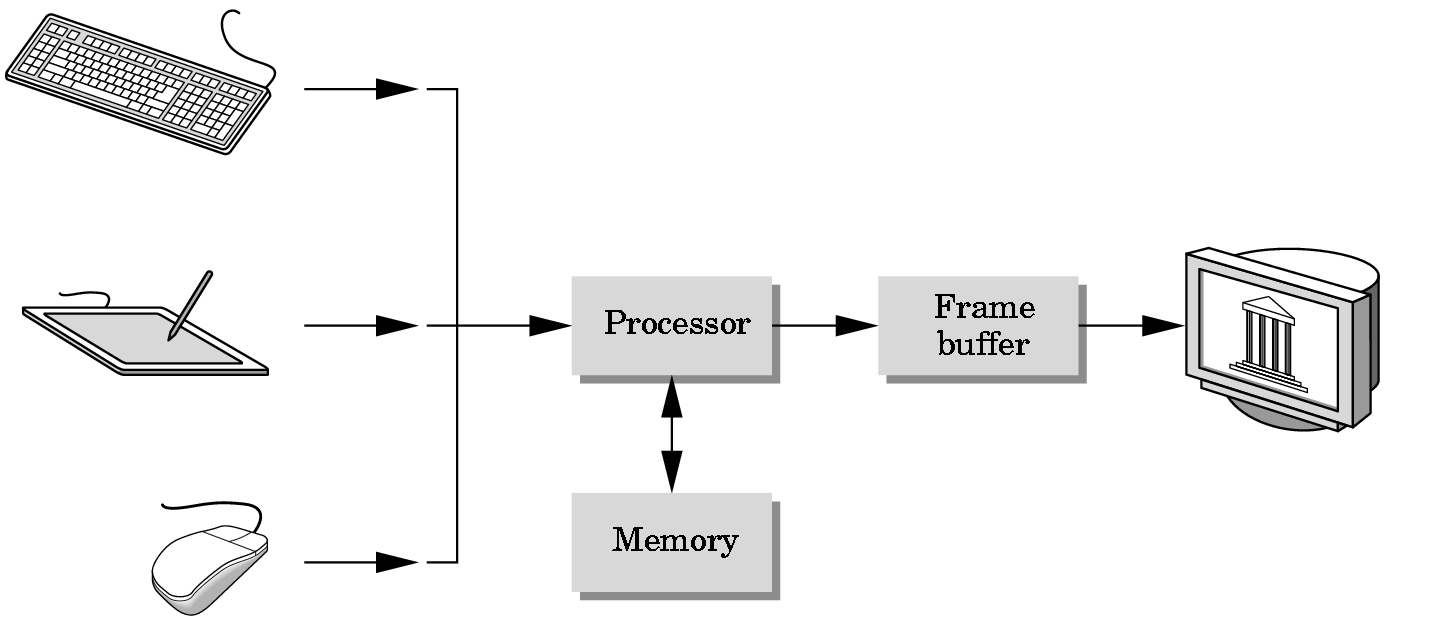
\includegraphics[scale=0.2]{img.png}
		\end{figure}
		\begin{center}
			\begin{tikzpicture}[>=latex, scale=.6]
			\draw (3,-3) -- (4,-2) -- (4,0) -- (2,0) -- (1,-1) ;
			\draw (3,-1) -- (4,0);
			\draw  (1,-1) rectangle (3,-3);
			\node [below] at (2,-3.5) {model};
			\draw[->] (4.5,-2) -- node[above, align=center] {graphics\\software} (6.5,-2);
			\foreach \i in {0.0, -0.5,..., -3}{
				\draw[fill=black] (7.5, \i) rectangle (7.1, \i-0.4);
				\foreach \x in {7.5,8,...,10.5}{
					\draw (\x, \i) rectangle (\x-0.4, \i-0.4);
					\draw[fill=black] (\x, -2) rectangle (\x-0.4, -2.4);
				}
			}
			
			
			\node [below] at (9,-3.5) {frame buffer};
			\draw[->] (11,-2) -- node[above, align=center] {graphics\\hardware} (13,-2);
			\draw (14,0) rectangle (18,-3) ;
			\node [below] at (16,-3.5) {monitor screen};
			\draw (18, -3) -- (19, -2) -- (19, 1) -- (15, 1) -- (14, 0);
			\draw (18,0) -- (19,1);
			\draw[fill=black] (14.5,-0.5) rectangle (17.5,-2.5);
			\draw[fill=white] (16.5,-2.5) -- (17,-2) -- (17,-1) -- (16,-1) -- (15.5,-1.5);
			\draw[fill=white] (15.5,-1.5) rectangle (16.5,-2.5);
			\draw (17,-1) -- (16.5,-1.5);
			
		\end{tikzpicture}
		\end{center}
		
		\noindent
		Le immagini raster sono \textbf{matrici} che contengono valori che rappresentano il colore
		nella casella corrispondente agli indici con valori discretizzati.
		
		\noindent
		Di solito ci sono componenti di colore: i monitor generano il colore
		con sovrapposizione di luce rossa, verde e blu (Perché?)
		
		\noindent
		Caratteristiche principali (non le uniche): 
		\begin{itemize}
			\item \textbf{risoluzione} (dimensioni della matrice di pixel)
			\item \textbf{profondità di colore} (bit di memoria per pixel).
		\end{itemize}
		8-bit significano 256 colori, mentre 24-bit (o truecolor)
		rappresentano all’incirca 32 milioni di colori
		
		\noindent
		\textbf{Nota}: è la rappresentazione di uscita tipica di quasi tutti i
		display odierni, ma non è ovviamente l'unica possibile
		\begin{itemize}
			\item Es.: display vettoriali: riproducono disegni
			\item Il formato digitale creato internamente deve ovviamente
			corrispondere alla capacità del display scelto di riprodurlo
		\end{itemize}
		
		Nel processo di rasterizzazione delle immagini vettoriali la qualità della
		conversione dipende	dalla risoluzione dell'immagine originale (numero di punti o punti per pollice).
		
		\noindent
		Un effetto possibile può essere la scalettatura: effetto dell'\textbf{aliasing} delle alte frequenze.
		Si può ridurre tale effetto sfumando la luminosità e facendo quindi \textit{antialiasing}.
		
		\begin{figure}[h!]
			\centering
			
\includegraphics[scale=0.2]{alias.png}
			\hspace*{0.4cm}
			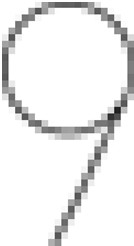
\includegraphics[scale=0.2]{alias1.png}
			\hspace*{0.4cm}
			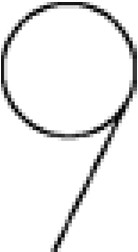
\includegraphics[scale=0.2]{alias2.png}
			\hspace*{0.4cm}
			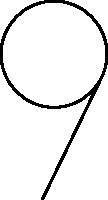
\includegraphics[scale=0.25]{alias3.png}
		\end{figure}
		
	\subsection{Aliasing}
		L'aliasing accade perché l'immagine è il campionamento di un segnale "continuo" che rappresenterebbe il dato misurabile.
		\[
			I(i, j) = I(i\Delta x, j\Delta y) = \iint F (x, y)\delta (x - i\Delta x)\delta (y - i\Delta y)
		\]
		
		\begin{center}
			\begin{tikzpicture}[>=latex, scale=0.5]
			\foreach \x in {0, 1, ..., 5}{
				\foreach \i in {0, -1, ..., -5}{
					\fill (\x,\i) circle (4pt);
				}
			}
			\draw[<->] (-0.5,-5) -- node[left] {$ \Delta y$} (-0.5,-4);
			\draw[<->] (0,-5.5) -- node[below] {$ \Delta x$} (1,-5.5);
		\end{tikzpicture}
		\end{center}
		
		Per il \textit{teorema di Shannon/Nyqvist} del campionamento, non si
		può ricostruire esattamente il segnale originale se la frequenza
		del segnale è superiore alla metà della frequenza di
		campionamento.
		
		\[
			v_{cx} = \dfrac{1}{\delta x} \geq 2v_{x max} \qquad 
			v_{cy} = \dfrac{1}{\delta y} \geq 2v_{y max} 
		\]
		
		Dove ci sono discontinuità del colore, ci sono componenti a
		frequenza alta, si creano artefatti. I filtri che fanno antialiasing attenuano le alte frequenze.
		
		
	\subsection{Caratteristiche Immagini raster}
		Le principali caratteristiche delle immagini raster sono:
		\begin{itemize}
			\item \underline{Risoluzione} (numero di righe e colonne matrice)
			\item \underline{Range dinamico}: rapporto tra minima differenza misurabile o
			rappresentabile e range di variabilità del segnale (luminosità). Corrisponde al numero di bit con cui codifichiamo il valore. Tipicamente 8 bit ma si può andare oltre:
			\begin{itemize}
				\item Immagini HDR
				\item Immagini mediche
				\item Dato che l'occhio umano non distingue così tante sfumature, lo
				scopo è di poter creare da esse rendering diversi che possano dare
				differenti effetti o informazioni
			\end{itemize}
			Il valore codificato dovrebbe corrispondere alla luminosità del
			punto generata dal monitor o acquisita dal sensore, ma la cosa
			è un po' più complicata a causa della \textbf{non-linearità della
			percezione umana}.
		\end{itemize}
		Insomma quello che c'è nel file non è quello che vediamo. Il rendering ed il dispositivo determinano la visualizzazione. E poi c'è il fattore legato alla percezione umana. 
		Ad esempio: immagini ad alto range dinamico (HDR) (Mantiuk et al 2005)
		
		\noindent
		La percezione umana amplifica le differenze del range dinamico ai bassi livelli. Macchine fotografiche e monitor applicano correzioni (gamma correction)
		
		\subsubsection{Colore}
			Le immagini raster da inviare ai display sono in genere a colori,
			per simulare il modo in cui vediamo il mondo (a colori).
			La rappresentazione del colore è generalmente una \textit{terna di
			valori RGB}.
			Per la riproduzione corrispondono alle intensità emesse da tre
			emettitori di luce a tre frequenze determinate (rosso, verde,
			blu) che danno origine in corrispondenza a un certo colore
			percepito dall'utente.
			
			\noindent
			\textit{Ma cosa significa questo?}
			
			\noindent
			Nei monitor si generano i colori nei punti della griglia per
			sintesi additiva: si mescolano due o più fasci luminosi di
			diversa.
			
			\noindent
			Nella stampa per sintesi sottrattiva: Due o più inchiostri
			sovrapposti assorbono diverse frequenze e cambiano la luce
			diretta all'occhio.
			
			\noindent
			Non tutti i colori possono essere generati in mescolanza
			additiva o sottrattiva di tre colori primari
			La scelta di \textbf{Rosso Verde Blu} come \textit{primari additivi} e \textbf{Giallo,
			Magenta e Cyan (e nero)} \textit{sottrattivi} cerca di massimizzare i
			colori rappresentabili.
			
			\begingroup
			\setlength\intextsep{0pt}
			\begin{wrapfigure}[13]{I}{0pt}
				% RGB color mixing
% Author: Henrik Skov Midtiby <http://midtiby.blogspot.com/>
\documentclass{standalone}
% Set target color model to RGB
\usepackage[rgb]{xcolor}
\usepackage{tikz}
\begin{document}

\begin{tikzpicture}[scale=0.5,  every node/.style={scale=0.8}]
% Create the background in the circle, by drawing several slices
% each with a constant color given by the angle (which is converted
% to a color usin the hue, saturation and brightness color space).
\foreach \x in {0,0.0111,...,1} {
	\definecolor{currentcolor}{hsb}{\x, 1, 1}
	\draw[draw=none, fill=currentcolor]
		(-360*\x+88:2) -- (-360*\x+88:3.8)
		-- (-360*\x+92:3.8) -- (-360*\x+92:2) -- cycle;
}

% On top of the background draw three spotlights of the primary colors
% red, green and blue (they are primary in an additive colorspace where
% light are mixed)
\draw [draw=none, fill=red] (90:1.5) circle (2cm);
\draw [draw=none, fill=green] (-30:1.5) circle (2cm);
\draw [draw=none, fill=blue] (210:1.5) circle (2cm);

% Draw areas where two of the three primary colors are overlapping.
% These areas are the secondary colors yellow, cyan and magenta.
\begin{scope} % red + green = yellow
	\clip (90:1.5) circle(2cm);
	\draw [draw=none, fill=yellow] (-30:1.5) circle (2cm);
\end{scope} % blue + red = magenta
\begin{scope}
	\clip (210:1.5) circle(2cm);
	\draw [draw=none, fill=magenta] (90:1.5) circle (2cm);
\end{scope}
\begin{scope} % green + blue = cyan
	\clip (-30:1.5) circle(2cm);
	\draw [draw=none, fill=cyan] (210:1.5) circle (2cm);
\end{scope}

% Draw the center area which consists of all the primary colors.
\begin{scope} % red + green + blue = white
	\clip (90:1.5) circle(2cm);
	\clip (210:1.5) circle(2cm);
	\draw [draw=none, fill=white] (-30:1.5) circle (2cm);	
\end{scope}

% Draw a circle with markings along the perimeter, indicating which angles
% the hue function connects to certain colors.
\draw (0, 0) circle (3.9cm);
\foreach \x  in {0, 30, ..., 330}
	\draw (-\x+90:3.8) -- (-\x+90:4.0) (-\x+90:4.4) node {$\x^\circ$};

% Add labels with names of the primary and secondary colors.
\foreach \x/\text in {0/red, 60/yellow, 120/green, 180/cyan, 240/blue, 300/magenta}
	\draw (-\x+90:5.5) node {\text};
\end{tikzpicture}


\end{document}
				\vspace{-50pt}
			\end{wrapfigure}
			
			
			\noindent
			L'uso delle 3 componenti di colore RGB è
			convenzionale e deriva dalla fisiologia della
			visione, che mostra che con 3 colori base si
			possono approssimativamente riprodurre i
			colori del mondo reale.
			
			\noindent
			I colori visibili però derivano invece da una
			variazione continua di lunghezza d'onda delle
			radiazioni elettromagnetiche in un intervallo
			percettibile di valori circa 370-730 nm.
			
			\noindent
			\textbf{Percezione del colore}: nella retina ci sono 3 tipi di coni, che
			hanno differenti sensitività a diverse frequenze S,M,L
			Possiamo fare il matching delle frequenze con la risposta dei
			recettori.
			
			\bigskip
			
			Il "colore" percepito è dato da 3 grandezze scalari, funzione
			dello spettro della luce incidente.
			La corrispondenza non è iniettiva. Spettri diversi possono
			corrispondere allo stesso colore percepito: metamerismo
			Conseguenza: Per riprodurre un colore, non è necessario
			riprodurre lo spettro. È sufficiente che le risposte L, M, S dei
			coni siano uguali.
			Può cambiare in funzione dell'illuminazione.
			
			
			\noindent
			\textbf{Metamerismo}: consiste nella possibilità di ottenere un effetto ottico tale che l'occhio percepisca la stessa sensazione di colore in presenza di luce con distribuzione spettrale diversa dal colore puro in questione.
			Si tratta di un'illusione ottica basata sulla natura dell'interpretazione del colore da parte dell'occhio umano, è possibile creare la sensazione di un colore "puro", formato, selezionando la sola lunghezza d'onda che genera quella determinata sensazione di colore miscelando a dovere più lunghezze d'onda differenti, un esempio è il bianco di una lampada fluorescente formato da spettri non uniformi, in questo caso la temperatura di colore che si trova sulle confezioni è la temperatura a cui deve essere un corpo nero perché l'occhio umano percepisca la stessa sensazione di colore.
			Il fenomeno si ha quando colori che appaiono all'occhio identici sotto una certa luce, mostrano tonalità differenti se illuminati con una luce diversa. In sostanza c'è metamerismo quando due colori si equivalgono sotto una fonte di luce, ma risultano differenti ad altre esposizioni.
			\endgroup
		\subsubsection{Legge di Grassman}
			L'uomo è in grado di fare match di colori mischiando 3 (o
			più) colori detti primari. Se la luce test $ T $ ha un certo colore:
			\[
				T = aP1 + bP2 + cP3
			\]
			il match si verifica lineare.
			\vspace{-0.25cm}
			
		\subsubsection{Funzioni di Matching}
			Data una terna di colori di base possiamo studiare il matching
			dei colori sugli osservatori in funzione della frequenza.
			Componenti colore CIERGB ricavate dall'integrale delle
			frequenze dello stimolo su tutto il range.
			\vspace{-0.5cm}
			\begin{align*}
				L &= \int \Phi (\lambda) L (\lambda) \diff\lambda \\
				M &= \int \Phi (\lambda) M (\lambda) \diff\lambda \\
				S &= \int \Phi (\lambda) S (\lambda) \diff\lambda 				
			\end{align*}
			
			Rappresentazione con matrice:
			\[
			C =
			\begin{pmatrix}
			\overline{r} (\lambda_1) & \dots & \overline{r}(\lambda_N) \\
			\overline{g} (\lambda_1) & \dots & \overline{g}(\lambda_N) \\
			\overline{b} (\lambda_1) & \dots & \overline{b}(\lambda_N) 
			\end{pmatrix}
			\]
			\[
			\Phi =
			\begin{pmatrix}
			\phi(\lambda_1)\\
			\vdots \\
			\phi (\lambda_N) 
			\end{pmatrix}
			\]
			
	\section{Schema di un'applicazione grafica}
		Vi è una descrizione di qualche tipo (procedurale o meno) del
		mondo che deve essere rappresentato. La produzione di tale
		descrizione (modello) prende il nome di \textbf{modellazione}.
		
		\noindent
		Da tale descrizione si ottiene una immagine visualizzabile da
		un display tale processo è chiamato globalmente \textbf{rendering}.
		
		\noindent
		La sequenza di procedure ed algoritmi che implementano il
		rendering prende il nome di \textbf{pipeline grafica}.
		
		\noindent
		Se l'applicazione è interattiva, il disegno dev'essere riprodotto
		in real time mentre l'utente interagisce con la scena mediante
		dei dispositivi.
			
	\subsection{Modello della scena}
		Nelle applicazioni 2D può essere un disegno da riprodurre sul
		display a meno di una trasformazione geometrica e mappatura
		sui pixel.
		Nelle applicazioni 3D di cui ci interesseremo sarà invece un
		vero e proprio modello del "mondo" che vogliamo vedere (e
		con cui vogliamo interagire) e l'immagine sarà generata
		simulando il processo di acquisizione di immagini di una
		telecamera "virtuale".
		
		\noindent
		Dati gli oggetti della scena, quindi dovremo "simulare" la geometria
		e la fisica della formazione delle immagini (luce, colore)
		
	\subsection{Rendering della scena}
		Il passaggio dalla rappresentazione all'immagine si definisce
		\textit{rendering}.
		
		\noindent
		Comprende tutti gli algoritmi per creare l'immagine per il
		display, che supporremo voglia un'immagine raster.
		
		\noindent
		Quindi se partiamo da una \textbf{rappresentazione 2D} (grafica
		vettoriale) il rendering consiste in:
		\begin{enumerate}
			\item Trasformazione delle primitive in rappresentazioni di colore sui pixel
			(rasterizzazione)
			\item Eventuale modifica interattiva del disegno
		\end{enumerate}
		Se partiamo da una \textbf{rappresentazione di scena 3D} il rendering consiste in:
		\begin{enumerate}
			\item Proiezione della scena sul piano immagine della telecamera virtuale
			\item Trasformazione della scena proiettata in rappresentazioni di colore
			sui pixel (rasterizzazione)
			\item Eventuale interazione con la scena e conseguenteupdate del
			rendering
		\end{enumerate}
		
		Il rendering comprende molti calcoli da svolgere, la \textbf{complessità} dipende dall'applicazione di interesse:
		\begin{itemize}
			\item Applicazioni interattive, real-time:
			\begin{itemize}
				\item Frame rate alto (>10 fps)
				\item Tempo di rendering del singolo frame prefissato
				\item Si può/deve sacrificare la qualità per garantire l’interattività
			\end{itemize}
			\item Applicazioni non interattive (computer animation, grafica
			pubblicitaria)
			\begin{itemize}
				\item l'obiettivo primario: massima qualità delle immagini di sintesi
				\item Non si hanno vincoli sul tempo di generazione del singolo frame
				\item Animazioni calcolate frame by frame da PC cluster, ricomposte
				successivamente nella successione temporale corretta
			\end{itemize}
		\end{itemize}
		
		Come si implementa la fase di rendering?
		\begin{itemize}
			\item Applicazioni interattive: si avvalgono pesantemente delle moderne schede grafiche (HW
				dedicato al processing di dati 3D)
			\item Applicazioni non interattive: fanno uso di ambienti di rendering più sofisticati e flessibili (ad es. RenderMan), spesso eseguiti SW su cluster di PC
		\end{itemize}
		
	\section{Modellare lo spazio}
		Richiamiamo le nozioni basilari di geometria per modellare lo
		spazio e gli oggetti:
		\begin{itemize}
			\item \textbf{Scalari}: unidimensionali, possono rappresentare grandezze fisiche
			con numeri
			\item \textbf{Punti}: rappresentano una posizione nello spazio
			\item \textbf{Vettori}: rappresentano le direzioni o le distanze tra punti in 2D o 3D
		\end{itemize}
		Per definire una posizione nello spazio dobbiamo introdurre un
		sistema di riferimento con un punto fisso detto origine e una
		terna di direzioni ortogonali
		
		\subsection{Scalari}
			Gli scalari S costituiscono un corpo (tipicamente useremo IR)
			con due operazioni, somma e moltiplicazione, che soddisfano
			le seguenti relazioni:
			
			\begin{multicols}{2}
				\begin{center}
					$ \forall \alpha,\beta,\gamma \in S $
				
				\noindent
				\textbf{Commutatività}
				\begin{align*}
					\alpha + \beta &= \beta + \alpha \\
					\alpha \beta &= \beta\alpha
				\end{align*}
				
				\textbf{Associatività}
				\begin{align*}
					\alpha + (\beta + \gamma) &= (\beta + \alpha) + \gamma \\
					(\alpha\beta)\gamma &= \alpha(\beta\gamma)
 				\end{align*}
				
				\textbf{Distribuzione}
				\[
					\alpha(\beta + \gamma) = \alpha\beta + \alpha\gamma
				\]
				
				\columnbreak
				
				\textbf{Elementi neutri}
				\begin{align*}
					\exists 0 \in S \: &: \: \forall \alpha \in S \quad \alpha + 0 = \alpha \\
					\exists 1 \in S \: &: \: \forall \alpha \in S \quad \alpha 1 = \alpha 
				\end{align*}
				
				\textbf{Elementi inversi}
				\begin{align*}
				\forall \alpha \in S \quad & \exists (-\alpha) \in S \: : \: \alpha + 0 = \alpha \\
				\forall \alpha \in S \quad & \exists \alpha^{-1} \in S \: : \: \alpha\alpha^{-1} = 1 
				\end{align*}
				\end{center}
			\end{multicols}
			
		\subsection{Vettori}
			I vettori costituiscono un \textbf{gruppo
			abeliano} (commutativo) $ V $ in cui e
			definito il \textbf{prodotto di un vettore
			per uno scalare}.
		
			\begin{multicols}{3}
				\begin{center}
				\textbf{Chiusura}
				\begin{align*}
					\vec{u} + \vec{v} \in V &\quad \forall \vec{u}\vec{v} \in V \\
					\alpha \vec{v} \in V &\quad \forall \alpha \in S \: \vec{v} \in V
				\end{align*}
				\columnbreak
				
				\textbf{Proprietà Algebriche}
				\begin{align*}
					\vec{u} + \vec{v} &= \vec{v} + \vec{u} \\
					\vec{u} + (\vec{v} + \vec{w}) &=  (\vec{u} + \vec{v}) + \vec{w} \\
					\alpha(\vec{u} + \vec{v}) &= \alpha\vec{u} + \alpha\vec{v} \\
					(\alpha + \beta)\vec{u} &= \alpha\vec{u} + \beta\vec{u}
				\end{align*}
				
				\begin{align*}
					\exists 0 &\in V \: : \: \forall \vec{u} \in V \quad \vec{u} + 0 = \vec{u} \\
					\forall \vec{u} &\in V \: \: \exists(-\vec{u}) \in V \: : \: \vec{u} + (-\vec{u}) = \vec{0}
				\end{align*}
			\end{center}
			\end{multicols}
		
			La definizione è totalmente
			astratta, ma per semplicità
			conviene considerare due utili
			esempi di spazi vettoriali lineari: Geometrico e Algebrico.
			
			\noindent
			Un esempio concreto e dato
			dai segmenti orientati liberi,
			ovvero senza un punto di
			applicazione specificato
			Il prodotto con uno scalare
			(numeri reali) cambia la
			lunghezza del vettore.
			La somma di due vettori e
			data dalla regola del
			parallelogramma.
			
			\begin{tikzpicture}[>=latex, baseline=0.5cm]
				\draw[thick, ->] (0,-2) -- (2,0) node[midway, left] {$ \vec{v} $};
				\draw[thick, ->] (0,-3) -- (3,0) node[midway, left] {$ 2\vec{v} $};
			\end{tikzpicture}
			\hspace*{0.5cm}
			\begin{tikzpicture}[>=latex, baseline=0.5cm]
				\draw[thick, <-] (0,-2) -- (2,0) node[midway, left] {$ -\vec{v} $};
				\draw[thick, ->] (4,-2) -- (6,0) node[midway, left] {$ \vec{v} + \vec{u} $};
				\draw[thick, ->] (4,-2) -- (5.5,-1.5) node[midway, below] {$ \vec{v}$};
				\draw[thick, ->] (5.5,-1.5) -- (6,0) node[midway, right] {$ \vec{u} $};
			\end{tikzpicture}
			
			\vspace*{0.5cm}
			
			\noindent
			Un altro esempio è dato dall'insieme delle n-ple ordinate di $ \R^n $.
			\[
				\vec{v} = (\beta_1, \dots, \beta_n) \quad \beta_i \in \R \forall i
			\]
			Il prodotto per uno scalare e la somma di due vettori sono
			definiti in modo del tutto naturale:
			\begin{align*}
				(\alpha_1, \dots, \alpha_n) + (\beta_1, \dots, \beta_n) &= 
				(\alpha_1 + \beta_1, \dots, \alpha_n + \beta_n) \\
				\alpha(\beta_1, \dots, \beta_n) &= (\alpha\beta_1, \dots, \alpha\beta_n)
			\end{align*}
			E' facile vedere qual è l'elemento neutro e qual è l'inverso di un
			vettore.
			
		\subsubsection{Indipendenza lineare}
			Dati n vettori non nulli, si dicono \textbf{linearmente indipendenti} se
			qualsiasi loro combinazione lineare a coefficienti non tutti nulli
			è diversa dal vettore nullo.
			\[
				\alpha_1\vec{v}_1 + \dots + \alpha_n \vec{v}_n = \vec{0} \: \Leftrightarrow \: \alpha_i = 0 \forall i
			\]
			Si dice \textbf{dimensione} di uno spazio vettoriale il massimo numero
			di vettori linearmente indipendenti.
			
			\noindent
			In uno spazio vettoriale a dimensione n, un insieme di n vettori
			linearmente indipendenti si dice una \textbf{base} per lo spazio.
			Ogni vettore può essere scritto come combinazione lineare dei
			vettori di una base.
		\subsubsection{Rappresentazione in componenti}
			Fissata quindi una \textbf{base in uno spazio vettoriale}, ad ogni
			vettore corrisponde una n-pla di scalari, ovvero i coefficienti
			dello sviluppo lineare del vettore nei vettori di base; tali scalari
			sono le componenti del vettore rispetto alla base data.
			
			\noindent
			In genere il corpo è dato dai reali; abbiamo quindi ottenuto la
			rappresentazione concreta vista prima di uno spazio vettoriale
			astratto come insieme di n-ple di $ \R^n $.
			Tale rappresentazione dipende dalla base scelta.
			
		\subsection{Punti}
			I vettori non rappresentano punti nello spazio, ma solo
			spostamenti. Per poter introdurre il concetto di \textbf{posizione} si
			deve passare agli \textbf{spazi affini} che sono degli spazi vettoriali a
			cui si aggiunge il concetto astratto di punto.
			
			\noindent
			I punti sono definiti in senso astratto come nuovi elementi con
			cui e possibile effettuare solo una operazione: la sottrazione
			tra punti.
			
			
			La differenza di due punti è un vettore: $ P - Q = \vec{v} $
			
			Dato un punto $ Q $ ed un vettore $ \vec{v} $, esiste un unico punto $ P $
			tale che $ P - Q = \vec{v} $.
			
			Si definisce quindi una somma tra un punto ed un vettore il
			cui risultato e un punto: $ P = Q + \vec{v} $
			
			\noindent
			\textit{Attenzione}: non ho sommato Q da entrambe le parti
			dell'equazione precedente.
			
			\noindent
			L'interpretazione geometrica è immediata; i punti sono
			locazioni nello spazio e la differenza di due punti e data dal
			vettore che li congiunge; è importante non confondere punti e
			vettori, sono entità geometriche ben distinte.
			
		\subsection{Combinazioni affini}
			Non è definita una somma tra punti e neppure un prodotto di
			uno scalare per un punto; in generale sono operazioni non
			lecite, ma c'è una eccezione.
			
			\noindent
			Si prendano tre punti P, Q ed O e si consideri il seguente
			punto: 
			\[
				P' = \alpha(P - O) + \beta(Q - O) + O 
			\]
			$ P' $ non dipende da $ O $, ma solo dai punti $ P $ e $ Q $, se e solo se $ \alpha + \beta = 1 $
			
			\noindent
			In questo caso $ P' $ è la \textbf{combinazione affine} di $ P $ e $ Q $, e si scrive,
			a volte in modo improprio, come \textbf{somma pesata dei punti}.
			
			\noindent
			\textit{La combinazione affine di due punti distinti descrive la retta
			passante per i due punti}.

			\noindent
			La combinazione affine si estende in modo naturale a $ n $ punti.
			\[
				P' = \sum_{i} \alpha_i P_i , \quad \sum_{i} \alpha_i = 1 \: \: \alpha_i \in \R
			\]
			Un insieme di punti si dice \textbf{affinemente indipendente} se
			\textit{nessun punto è combinazione affine degli altri}.
			
		\subsubsection{Combinazione Convessa}
			La combinazione convessa è una combinazione affine con pesi
			positivi.
			
			\noindent
			Nel caso della combinazione convessa di due
			punti, il punto risultante giace sul segmento
			che congiunge i due punti. Se i pesi sono
			entrambi pari a $ 0.5 $, il punto risultante si trova
			a metà tra i due.
			
			\begin{tikzpicture}[scale=0.7,baseline=0.5cm]
				\draw (0,-2) -- (2,0);
				\fill (0,-2) circle (2pt) coordinate [label=below:$P$] (a)
					  (2,0) circle (2pt) coordinate [label=above:$Q$] (b)
					  (1,-1) circle (2pt) coordinate [label=left:$\dfrac{P+Q}{2}$] (c);
			\end{tikzpicture}
			\hspace*{2.5cm}
			\begin{tikzpicture}[scale=0.7,baseline=0.5cm]
				\draw (0,-2) -- (1,0) -- (4,-2) -- cycle;
				\fill (0,-2) circle (2pt) coordinate [label=below:$P$] (a)
					(1,0) circle (2pt) coordinate [label=above:$Q$] (b)
					(4,-2) circle (2pt) coordinate [label=above:$R$] (c)
					(1.7,-1.3) circle (2pt) coordinate [label=left:$\dfrac{P+Q+R}{3}$] (d);
			\end{tikzpicture}
			
			\noindent
			Nel caso di $ n $ punti che formano un poligono
			convesso, il punto risultante si trova all'interno del poligono.
			Se tutti i pesi sono uguali a $ 1/n $, il punto risultante si chiama
			\textbf{centroide} dell'insieme dei punti.
			
		\subsubsection{Guscio Convesso}
			Un insieme $ C \in \R^n $ è convesso se per ogni coppia di punti $ P_1, P_2 \in C$ 
			si ha che $ P' = \alpha(P_1 - P_2 ) + P_2 $ appartiene
			a $ C $ per ogni $ \alpha \in [0, 1] $  ovvero tutti i punti sul segmento che
			unisce $ P_1 $ con $ P_2 $ appartengono all'insieme $ C $.
			
			\noindent
			Il guscio convesso (\textit{convex hull}) di un insieme di punti è la più
			piccola regione convessa che contiene tutti i punti dati.
			
		\subsection{Prodotto interno}
			In uno spazio affine non è ancora definito il concetto di
			distanza o di angolo tra vettori; questi si ottengono passando ad
			uno spazio euclideo che è uno spazio affine provvisto di
			un \textbf{prodotto interno tra vettori (\textit{prodotto scalare})} che è definito come:
			
			Dati due vettori $ a = [a_i]_1^n $ e $ b = [b_i]_1^n $ di $ \R^n $
			\[
				\sum_{1}^{n} a_i b_i = 
				\begin{bmatrix}
					a_1 & \dots & a_n
				\end{bmatrix}
				\begin{bmatrix}
					b_1 \\
					\vdots \\
					b_n
				\end{bmatrix}
				= a'b
			\]
			
			
			che soddisfa le seguenti relazioni:
			\begin{align*}
				\vec{u} \cdot \vec{v} &= \vec{v}\cdot \vec{u} \in S \\
				(\alpha\vec{u} + \beta\vec{v}) \cdot\vec{w} &= 
				\alpha\vec{u}\cdot\vec{w} + \beta\vec{v}\cdot\vec{w} \\
				\vec{v}\cdot\vec{v} > 0 & \: \: (\vec{v} \neq \vec{0}) \\
				\vec{0}\cdot\vec{0} &= 0
			\end{align*}
			
			Se il prodotto interno di due vettori è nullo, diremo che i \textbf{due
			vettori sono ortogonali}. 
			Grazie al prodotto interno e possibile definire la \textbf{lunghezza di
			un vettore} (e quindi la distanza tra due punti) e l'\textbf{angolo} tra
			due vettori.
			
			\noindent
			\textbf{Norma di un vettore}:
			\[
				\lVert \vec{v} \rVert = \sqrt{\vec{v}\cdot\vec{v}} \quad 
				\cos \theta = \dfrac{\vec{v}\cdot\vec{u}}{\lVert \vec{v} \rVert \: \lVert \vec{u} \rVert}
			\]
			
			Il prodotto scalare può essere usato, ad esempio, per trovare la
			proiezione di un vettore lungo una retta.
			Sia dato il vettore $ \vec{v} $ e la retta con direzione identificata dal
			vettore di lunghezza unitaria $ u $; il vettore ottenuto proiettando
			v lungo la retta sarà della forma $ \vec{v}' = t\vec{u} $ dove $ t $ è un parametro,
			si può dimostrare che $ t = \vec{v} \cdot \vec{u} $
			
			\begin{center}
				\begin{tikzpicture}[>=latex]
				\draw (0,-2) -- (5,-2);
				\draw[ultra thick, ->] (1,-2) -- (2,-2) node[above] {$ \vec{u} $};
				\draw[ultra thick, ->] (1,-2) -- (4,-2) node[below] {$ (\vec{v}\cdot\vec{u})\vec{u} $};
				\draw[->] (1,-2) -- (4,0) node[outer sep=4pt,left] {$ \vec{v} $};
				\draw[dashed] (4,0) -- (4,-2);
			\end{tikzpicture}
			\end{center}
			
		\subsection{Normalizzazione}
			Un vettore è normalizzato se la sua lunghezza è $ 1 $; dato un
			vettore qualsiasi lo si può normalizzare moltiplicandolo per il
			reciproco della sua lunghezza.
			
			\noindent
			\textit{Un vettore normalizzato si dice anche \textbf{versore}}
			
			Una base è \textbf{ortonormale} se e formata da versori a due a due
			ortogonali:
			\[
				(e_1, \dots, e_n) \: : \: \lVert e_i \rVert = 1 \: \forall i \quad \textup{e}
				\quad e_i\cdot e_j = 0 \quad \forall i \neq j
			\]
			Data una base ortonormale il prodotto interno tra due vettori
			si esprime come somma dei prodotti delle componenti (usuale
			prodotto scalare di vettori)
			\[
				\vec{v} \vec{w} = v_1 w_1 + \dots + v_n w_n
			\]
			data una base qualsiasi è sempre possibile derivare da essa una base
			ortonormale (procedimento di \textit{Gram-Schmidt})
			
		\subsection{Terne}
			In tre dimensioni una base ortonormale si dice \textbf{destrorsa}, se la
			rotazione attorno ad $ \vec{e}_3 $ che porta $ \vec{e}_1 $ a coincidere con $ \vec{e}_2 $ è
			antioraria se vista dalla parte positiva di $ \vec{e}_3 $ .
			Se tale rotazione è oraria allora la base è \textbf{sinistrorsa}.
			
			\noindent
			Si può usare la \textit{prima regola della mano destra}: se si pone il
			pollice nella direzione di $ \vec{e}_3 $ , la rotazione che porta $ \vec{e}_1 $ in $ \vec{e}_2 $ deve seguire il modo naturale con cui si piegano le altre dita.
			
			\noindent
			Oppure la \textit{seconda regola della mano destra} per determinare la
			destrorsità: se si riesce a porre i tre vettori di base in
			corrispondenza con pollice, indice e medio della mano destra,
			tenuti perpendicolari l'uno all'altro, la base e destrorsa.
			La scelta di un orientamento è del tutto arbitraria, basta
			essere coerenti. Di norma si usano basi destrorse.
			
		\subsection{Sistemi di riferimento (frame)}
			Il concetto di base si estende a quello di riferimento in uno
			spazio affine (o euclideo) specificando, oltre alla base, anche
			un punto $ O $ detto origine del riferimento.
			
			\noindent
			Poiché ogni vettore è sviluppabile in una base data ed ogni
			punto esprimibile come somma di un punto dato e di un
			vettore, dato un riferimento $ (\vec{e}_1, \vec{e}_2, \vec{e}_3, O) $, i punti ed i vettori
			dello spazio saranno esprimibili nel seguente modo:
			\begin{align*}
				\vec{v} &= v_1\vec{e}_1 + v_2\vec{e}_2 + v_3\vec{e}_3 \\
				P &= p_1\vec{e}_1 + p_2\vec{e}_2 + p_3\vec{e}_3 + O
			\end{align*}
			Un riferimento \textbf{cartesiano} è dato da un riferimento la cui base
			di vettori sia ortonormale. 
			
			\noindent
			Un riferimento è destrorso se lo è la sua base.
			
		\subsection{Coordinate omogenee}
			Definiamo il prodotto di un punto per 1 e per 0: $ \quad P\cdot 1 = P \quad P\cdot 0 = 0 $.
			
			In questo modo possiamo definire le coordinate omogenee di
			un punto e di un vettore rispetto al riferimento $ (\vec{e}_1 , \vec{e}_2 , \vec{e}_3 ,O) $.
			\begin{align*}
				\vec{v} &= (v_1, v_2, v_3, 0) \\
				P &= (p_1, p_2, p_3, 1)
			\end{align*}
			La scelta di 0 e 1 come ultima coordinata per vettori e punti è
			arbitraria, andrebbe bene qualsiasi valore:
			
			\noindent
			Tale scelta però permette il \textbf{type checking}: si trattano le 4-ple delle
			coordinate omogenee come vettori quando si effettua una qualsiasi
			combinazione lineare di punti e vettori, usando le usuali regole, se
			l'ultima coordinata del risultato è 0, allora il risultato è un vettore;
			se è pari a 1 allora il risultato è un punto!
			
			\noindent
			Se non è ne 0 ne 1, allora si è effettuata una operazione non lecita
		
		\subsection{Riepilogo}
		
		\begin{itemize}
			\item Gli scalari sono numeri reali
			\item I vettori identificano direzioni nello spazio
			\item I punti determinano posizioni nello spazio
			\item Operazioni ammesse:
			somma e prodotto tra scalari, prodotto di scalari per vettori, somma
			di vettori, differenza di punti, somma di un punto con un un vettore,
			combinazioni affini.
			\item Il prodotto scalare permette di determinare la lunghezza dei
			vettori, la distanza tra punti e l'angolo tra due vettori
			\item Conviene lavorare in una base ortonormale; in questo caso il
			prodotto scalare tra due vettori e particolarmente semplice
			\item I tre assi che formano la base si chiamano assi coordinati e si
			indicano con $ x, y $ e $ z $ (a volte useremo anche 1, 2 e 3).
		\end{itemize}
		
		\subsection{Prodotto vettore}
		Nel caso particolare delle tre dimensioni è utile introdurre
		un'ulteriore operazione tra vettori: \textbf{il prodotto vettore}.
		
		\noindent
		Si tratta di un caso particolare di prodotto denominato
		\textbf{esterno}; in tre dimensioni particolarmente semplice:
		\[
		\vec{u}\times\vec{v} = (u_y v_z - u_y v_y,\: u_z v_x - u_x v_z,\: u_x v_y - u_y v_x)
		\]
		Si dimostra che il prodotto vettore di due vettori $ \vec{u} $ e $ \vec{v} $ è un
		vettore ortogonale al piano contenente i due vettori e di
		modulo pari all'area definita da $ \vec{u} $ e $ \vec{v} $. Il verso è scelto in modo
		tale che $ (\vec{u}, \vec{v}, \vec{u} \times \vec{v}) $ formino una terna destrorsa.
				
		\noindent
		\textit{Attenzione}: il prodotto vettore (a differenza delle proprietà affini
		dello spazio) dipende dalla scelta del tipo di base, destrorsa o sin.
				
		\textbf{Esempio:} Data una direzione espressa dal vettore unitario $ \vec{v} $, voglio
		creare un sistema di riferimento ortogonale con l'asse $ z $
		coincidente con $ \vec{v} $. Come faccio?
		\begin{itemize}
			\item Prendo un qualunque vettore $ \vec{a} $ non parallelo a $ \vec{v} $.
			\item Prendo la direzione dell'asse $ x $ $ \vec{e}_1 $ uguale a $ \vec{v} \times \vec{a} $.
			\item Prendo la direzione dell'asse $ y $ $ \vec{e}_2 $ uguale a $ \vec{v} \times \vec{e}_1 $.
		\end{itemize}
				
	\subsection{Matrici e trasformazioni}
		Una matrice è essenzialmente un array bidimensionale di
		elementi; per i nostri scopi gli elementi saranno sempre degli
		scalari, tipicamente numeri reali.
		
		Una matrice $ A $ puo essere moltiplicata per uno scalare $ \beta $
		ottenendo una matrice $ C = \beta A $ definita nel seguente modo:
		\[
			c_{i j} = \beta a_{i j} \quad \forall i, j
		\]
		
		Due matrici $ A $ e $ B $ si possono sommare se e solo se hanno lo
		stesso numero di righe e di colonne; in tal caso si ha $ C = A + B $ data da:
		\[
			c_{i j} = a_{i j} + b_{i j} \quad \forall i, j
		\]
		
		Il prodotto tra matrici e definito solo quando il numero di
		colonne della prima matrice è uguale al numero di righe della
		seconda. Se $ A $ è una matrice $ N\times M $ e $ B $ e una matrice $ M\times K $, allora
		si ha $ C = AB $ (di dimensioni $ N\times K $) data da:
		\[
			c_{i j} = \sum_{l = 1}^{M} a_{i l} b_{l j}
		\]
		Il prodotto tra matrici è \textbf{associativo} ($ (AB)C = A(BC) $), ma \textbf{non commutativo} (in generale $ AB\neq BA $)
			
	\subsection{Matrice trasposta}
		Indicata con il simbolo $ A_T $ , è la matrice ottenuta scambiando le
		righe con le colonne di $ A $: 
		\[
			a_{i j}^T = a_{j i} 
		\] 
		Quindi se $ A $ è $ N\times M $, allora la sua trasposta è $ M\times N $.
		
		\noindent
		Per i vettori trasporre equivale a trasformare un vettore riga in
		un vettore colonna e viceversa
		D'ora in poi quando parleremo di \textbf{trasformazione} di un vettore
		$ \vec{v} $ con una matrice $ A $ intenderemo sempre l'usuale \textit{prodotto di
		matrici} tra $ A $ e il trasposto di $ \vec{v} $ inteso come matrice con una
		sola colonna, es.:
		\[
			A\vec{v} =
			\begin{pmatrix}
				a_{1 1} & a_{1 2} \\
				a_{2 1} & a_{2 2}
			\end{pmatrix}
			\begin{pmatrix}
				v_1 \\
				v_2
			\end{pmatrix}
			=
			\begin{pmatrix}
				a_{1 1}v_1 + a_{1 2}v_2 \\
				a_{2 1}v_1 + a_{2 2}v_2
			\end{pmatrix}
		\]
		
	\subsection{Determinante}
		Importante parametro per le matrici quadrate, indicato con il
		simbolo $ det A $ o con il simbolo $ |A| $. Si definisce
		ricorsivamente:
		
		Il determinante di una matrice $ 2x2 $ è definito da:
		\[
			\begin{vmatrix}
				a_{1 1} & a_{1 2} \\
				a_{2 1} & a_{2 2}
			\end{vmatrix}
			= a_{1 1}a_{2 2} - a_{1 2}a_{2 1}
		\]
		Il determinante di una matrice $ N\times N $ è dato dalla formula:
		\[
			detA = \sum_{j = 1}^{N} (-1)^{j + k} a_{j k} detA_{j k}
		\]
		dove $ k $ e una colonna qualsiasi di $ A $ e dove il simbolo $ A_{j k} $ indica
		la matrice $ (N-1)\times(N-1) $ ottenuta da $ A $ eliminando la riga $ j $ e la
		colonna $ k $. Si può dimostrare che $ det(AB) = detA\: detB $
		
		\noindent
		Si può dimostrare che una matrice e invertibile se e solo se il suo
		determinante è diverso da 0; in tal caso si ha:
		\[
			a_{i j}^{-1} = (-1)^{i+j} \dfrac{\textup{det}A_{i j}}{\textup{det}A}
		\]
	\subsection{Matrici: trasformazioni e cambiamento di base}
		Abbiamo visto cosa significa applicare una matrice ad un vettore
		\begin{itemize}
			\item Le matrici quadrate rappresentano quindi delle\textbf{ applicazioni
			lineari} di uno spazio vettoriale in sé (formano un gruppo non
			abeliano).
			\item Tutte le applicazioni lineari di uno spazio vettoriale in sé sono
			esprimibili tramite \textbf{matrici quadrate}.
			\item L'applicazione di più di una matrice ad un vettore si effettua
			sfruttando l'algebra delle matrici; ad esempio applicare prima
			$ A $, poi $ B $ ed infine $ C $ equivale ad applicare la matrice $ CBA $.
		\end{itemize}
		Abbiamo detto che dato uno spazio vettoriale esistono infinite
		basi. Nella rappresentazione concreta il \textbf{cambiamento da una
		base ad un'altra} è descritto da una matrice.
	
		\noindent
		In generale dato un vettore $ (v_1 , v_2 , v_3 ) $, la sua trasformazione
		in $ (v'_1 , v'_2 , v'_3 ) $ tramite la matrice $ M $ puo essere vista come :
		\begin{itemize}
			\item Una trasformazione identificata da M del vettore fissata la base (\textbf{trasformazione attiva}).
			\item Un cambiamento di base indotto dalla matrice $ M^{-1} $ tenendo fisso il vettore (\textbf{trasformazione passiva}).
		\end{itemize}
		
	\subsection{Cambio di riferimento}
		L'idea si ripropone negli stessi termini per i sistemi di
		riferimento.\\
		Dati due riferimenti $ (\vec{e}_1 , \vec{e}_2 , \vec{e}_3 ,O) $ e 
		$ (\vec{e'}_1 ,\vec{e'}_2 ,\vec{e'}_3 ,O) $ si tratta
		di trovare una matrice $ 4\times 4 $ che permetta di ottenere le
		coordinate di un punto rispetto al secondo riferimento date le
		coordinate dello stesso punto rispetto al primo.
		
		Come nel caso dei cambiamenti di base di un riferimento, se $ T $
		è la trasformazione attiva che manda il primo riferimento nel
		secondo (e che manda le coordinate rispetto al secondo nelle
		coordinate rispetto al primo), allora $ T_{-1} $ e la matrice che
		trasforma le coordinate rispetto al primo riferimento nelle
		coordinate rispetto al secondo riferimento.
		
		\textbf{Esempio: }\\
		Determinare la rotazione che porta gli assi canonici 
		$ \vec{e}_1 =(1,0,0),\: \vec{e}_2 = (0,1,0),\: \vec{e}_3=(0,0,1) $
		in una qualunque terna 
		\begin{align*}
			\vec{e'}_1 &=(e'_{11} ,e'_{12} ,e'_{13} ), \\
			\vec{e'}_2 &=(e'_{21} ,e'_{22} ,e'_{23} ), \\
			\vec{e'}_3 &=(e'_{31} ,e'_{32} ,e'_{33} ) 
		\end{align*}
		La matrice di rotazione è data da:
		\[
			\begin{pmatrix}
				\vec{e}_1\vec{e'}_1 & \vec{e}_1\vec{e'}_2 & \vec{e}_1\vec{e'}_3 \\
				\vec{e}_2\vec{e'}_1 & \vec{e}_2\vec{e'}_2 & \vec{e}_2\vec{e'}_3 \\
				\vec{e}_3\vec{e'}_1 & \vec{e}_3\vec{e'}_2 & \vec{e}_3\vec{e'}_3 \\
			\end{pmatrix}
		\]
		
	\subsection{Traslazione}
	
		Una traslazione determinata dal vettore $ \vec{t} $ trasforma il punto $ P $ nel punto:
		\begin{wrapfloat}{figure}{O}{0pt}
			\begin{tikzpicture}[>=latex, scale=0.7]
			\draw[ultra thick, ->] (4,-3) -- (1,-4) node[above, left] {$ x $};
			\draw[ultra thick, ->] (4,-3) -- (7,-4) node[above, right] {$ y $};
			\draw[ultra thick, ->] (4,-3) -- (4,0) node[left] {$ z $};
			\draw[->] (3,-2) -- node[above] {$ \vec{t} $} (6,-1) node[right] {$ P + \vec{t} $};
			\fill (3,-2) circle (2pt) coordinate [label=below:$P$] (a);
			\end{tikzpicture}
		\end{wrapfloat}
		\[
			P' = P + \vec{t}
		\]
		
		In termini di componenti:
		\begin{align*}
			\vec{t} &= (t_x, t_y, t_z, 0) \\
			P &= (p_x, p_y, p_z, 1) \\
			P' &= (p_x + t_x,\: p_y + t_y,\: p_z + t_z,\; 1 )
		\end{align*}
		E' facile vedere che la matrice di
		trasformazione T t per le coordinate
		omogenee è:
		
		\[
			T_t =
			\begin{pmatrix}
				1 & 0 & 0 & t_x \\
				0 & 1 & 0 & t_y \\
				0 & 0 & 1 & t_z \\
				0 & 0 & 0 & 1 \\
			\end{pmatrix}
		\]
		
	\begin{wrapfigure}{r}{0.35\textwidth}
		\vspace{-30pt}
		\begin{tikzpicture}[>=latex, scale=0.7]
		\draw[ultra thick, ->] (4,-3) -- (1,-4) node[above, left] {$ x $};
		\draw[ultra thick, ->] (4,-3) -- (7,-4) node[above, right] {$ y $};
		\draw[ultra thick, ->] (4,-3) -- (4,0) node[left] {$ z $};
		\draw[->] (4,-3) -- (2,-5) node[left] {$ P $};
		\draw[->] (4,-3) -- (6,-5) node[right] {$ P' $};
		\draw[->, bend right] (3,-4) to (5,-4) ;
		\node at (4,-4) {$ \theta $};
		\end{tikzpicture}
		\vspace{-40pt}
	\end{wrapfigure}
	
	\subsection{Rotazione}
		Una rotazione di un angolo $ \theta $ in
		senso \textbf{antiorario} (prima regola della
		mano destra) \textbf{intorno all'asse} $ z $
		determina la seguente trasformazione
		di un punto $ P $ in $ P' $.
		
		\begin{align*}
			p'_x &= p_x\cos(\theta) - p_y \sin(\theta) \\
			p'_y &= p_x\sin(\theta) + p_y \cos(\theta) \\
			p'_z &= p_z			
		\end{align*}
		
		Si può facilmente dimostrare che per rotazioni intorno
		all'asse $ x $ e $ y $ si hanno le seguenti espressioni:
			\begin{align*}
				p'_y &= p_y \cos(\theta) - p_z \sin(\theta) \qquad &
					\qquad p'_z &= p_z \cos(\theta) - p_x \sin(\theta) \\
				p'_z &= p_y \sin(\theta) - p_z \cos(\theta) \qquad &
					\qquad p'_x &= p_z \sin(\theta) - p_x \cos(\theta) \\
				p'_x &= p_x \qquad & \qquad p'_y &= p_y
			\end{align*}

		\noindent
		\textbf{Matrici} che rappresentano le rotazioni rispetto agli assi coordinati:
		\[
			R_x(\theta) =
			\begin{pmatrix}
				1 & 0 & 0 & 0 \\
				0 & \cos\theta & -\sin\theta & 0 \\
				0 & \sin\theta & \cos\theta & 0 \\
				0 & 0 & 0 & 1
			\end{pmatrix}
			\quad
			R_y(\theta) =
			\begin{pmatrix}
			\cos\theta & 0 & \sin\theta & 0 \\
			0 & 1 & 0 & 0 \\
			-\sin\theta & 0 & \cos\theta & 0 \\
			0 & 0 & 0 & 1
			\end{pmatrix}
			\quad
			R_z(\theta) =
			\begin{pmatrix}
			\cos\theta & -\sin\theta & 0 & 0 \\
			\sin\theta & \cos\theta & 0 & 0 \\
			0 & 0 & 1 & 0 \\
			0 & 0 & 0 & 1
			\end{pmatrix}
		\]
		\textbf{Osservazioni:}\\
		Da notare che un \textit{vettore viene
		trasformato da una rotazione} (a
		differenza delle traslazioni che
		lasciano i vettori inalterati). \textit{Le matrici non commutano}.
		
		\noindent
		Le rotazioni rispetto agli assi cartesiani non commutano;
		provare a ruotare un oggetto di 90 gradi prima rispetto all'asse
		x e poi rispetto all'asse y. Ripetete quindi l'operazione prima
		rispetto all'asse y e poi rispetto all'asse x. Risultato?
		
		\noindent
		Da notare che le rotazioni lasciano inalterati i punti che si
		trovano sull'asse di rotazione.
		
		Si può dimostrare che $ R_x(\theta)^{-1} = R_x(-\theta) $ e similmente per gli
		altri assi.
		
		Si può dimostrare che le matrici di rotazione date sopra sono
		\textbf{ortogonali},\\
		 ad es. per l'asse x: $ R_x(\theta)^{-1} = R_x(-\theta)^T $
		
		\textit{La proprietà di ortogonalità è vera per ogni rotazione, non solo
		per quelle rispetto agli assi coordinati}.
		Tutte le rotazioni sono esprimibili con matrici.
		
	\subsection{Composizione di trasformazioni di matrici}
		Le trasformazioni espresse come matrici si compongono
		usando semplicemente l'algebra delle matrici.
		Date due trasformazioni rappresentate dalle matrici $A$ e $B$, la
		composizione di $A$ seguita da $B$ sarà data dalla matrice $BA$.

		\noindent
		\textbf{Importante}: notare l'ordine delle matrici; siccome si applica la
		matrice risultante a sinistra del vettore delle coordinate omogenee,
		la trasformazione che viene effettuata per prima va a destra.
		La composizione di trasformazione si estende immediatamente
		al caso di piu di due matrici: $T = T_n \dots T_1$

	\subsection{Non commutatività}
		Esempio: data una traslazione lungo il vettore $\vec{t}$ ed una rotazione di un angolo lungo
		l'asse $\vec{z}$, si ottiene un risultato diverso effettuando prima la rotazione e poi la traslazione o
		viceversa.

		Per rendersene conto basta guardare come viene trasformato nei due casi un punto che in partenza si trova
		nell'origine.

		\begin{tikzpicture}[>=latex]
			\draw[thick, ->] (0,-.25) -- (0,2) node[anchor=north east] {y};
			\draw[thick, ->] (-.25,0) -- (3,0) node[anchor=north west] {x};
			\draw[ultra thick, ->] (0,0) -- (2,0);
			\draw[ultra thick, ->] (0,0) -- (1.5,1.5);
			\draw[->,bend right] (1,0) to (0.65,0.65) node[right, outer sep=4pt] {$ R(\theta) $};
			\node[below] at (1,0) {$\vec{t}$};
			\node at (3,2) {$ R(\theta)M_t $};
			\fill[blue] (1.5,1.5) circle (3pt);
			\node[left] at (1.5, 1.5) {$ P' $};
			\fill[blue] (0,0) circle (3pt); 
			\node at (-0.2,0.2) {$ P $};
		\end{tikzpicture}
		\hspace{1.5cm}
		\begin{tikzpicture}[>=latex]
			\draw[thick, ->] (0,-.25) -- (0,2) node[anchor=north east] {y};
			\draw[thick, ->] (-.25,0) -- (3,0) node[anchor=north west] {x};
			\draw[ultra thick, ->] (0,0) -- (2,0);
			\draw[->,bend right] (1,0) to (0.65,0.65) node[right, outer sep=4pt] {$ R(\theta) $};
			\node[below] at (1,0) {$\vec{t}$};
			\node at (3,2) {$ M_t R(\theta) $};
			\fill[blue] (0,0) circle (3pt); 
			\fill[blue] (2,0) circle (3pt); 
			\node at (-0.2,0.2) {$ P $};
			\node[above] at (2,0) {$ P' $};
		\end{tikzpicture}
		
	\subsection{Scalatura}
		Traslazioni e rotazioni conservano la lunghezza dei vettori e sono un
		 sottogruppo delle trasformazioni affini chiamato trasformazioni isometriche o rigide.
		Un altro tipo di trasformazione affine che non preserva le
		distanze è la \textbf{scalatura}.
		
		\noindent
		Dato un punto $ P = (p_x, p_y, p_z, 1) $ la trasformazione di scala, o scalatura, lo trasforma nel punto $ P' = (s_x p_x, s_y p_y, s_z p_z, 1) $ dove i valori $ (s_x, s_y, s_z) $ sono i fattori di scala lungo gli assi.
		
		\noindent
		Una scalatura è \textit{omogenea} se $ s_x = s_y = s_z = s $ 
		
		\begin{itemize}
			\item vettori semplicemente allungati ($ s>1 $) o accorciati ($ s<1 $).
			\item Un punto, in una scalatura omogenea, viene invece traslato lungo la
				retta che passa per l'origine e per il punto stesso.
		\end{itemize}
		
	\subsection{Trasformazioni affini}
		Una generica matrice che lavora in coordinate omogenee
		rappresenta una trasformazione affine (12 gradi di libertà non
		solo traslazione rotazione e scala, ma anche shear)
		\[
		\begin{pmatrix}
			x \\
			y \\
			z
		\end{pmatrix}
		\mapsto
		\begin{pmatrix}
			a & b & c \\
			d & e & f \\
			g & h & i
		\end{pmatrix}
		\begin{pmatrix}
			x \\
			y \\
			z
		\end{pmatrix}
		+
		\begin{pmatrix}
			u \\
			v \\
			w
		\end{pmatrix}
		\]
		Se t è il vettore di traslazione e R una matrice di rotazione, la
		trasformazione in coordinate omogenee è:
		\[
			\begin{pmatrix}
				R & t \\
				0 & 1
			\end{pmatrix}
		\]
	\subsection{Rotazioni generiche e orientazione}
		Dobbiamo considerare rotazioni attorno a qualunque asse.
		Comunque, non c'è nessuna perdita di generalità nel definirle
		solo attorno agli assi passanti per l'origine, dato che le altre le
		posso ricavare traslando l'origine sull'asse, ruotando e
		ritraslando l'origine all'indietro.
		
		\noindent
		La rotazione rappresenta un cambio di orientazione
		L'orientazione rappresenta la posa di un oggetto nello spazio
		La relazione che c'è tra rotazione (movimento) e orientazione
		(stato) è analoga a quella tra punto e vettore
		Anche per le operazioni:
		\begin{itemize}
			\item orientazione+rotazione=orientazione
			\item rotazione+rotazione=rotazione
		\end{itemize}
		
		\begin{SCfigure}[][h!]
			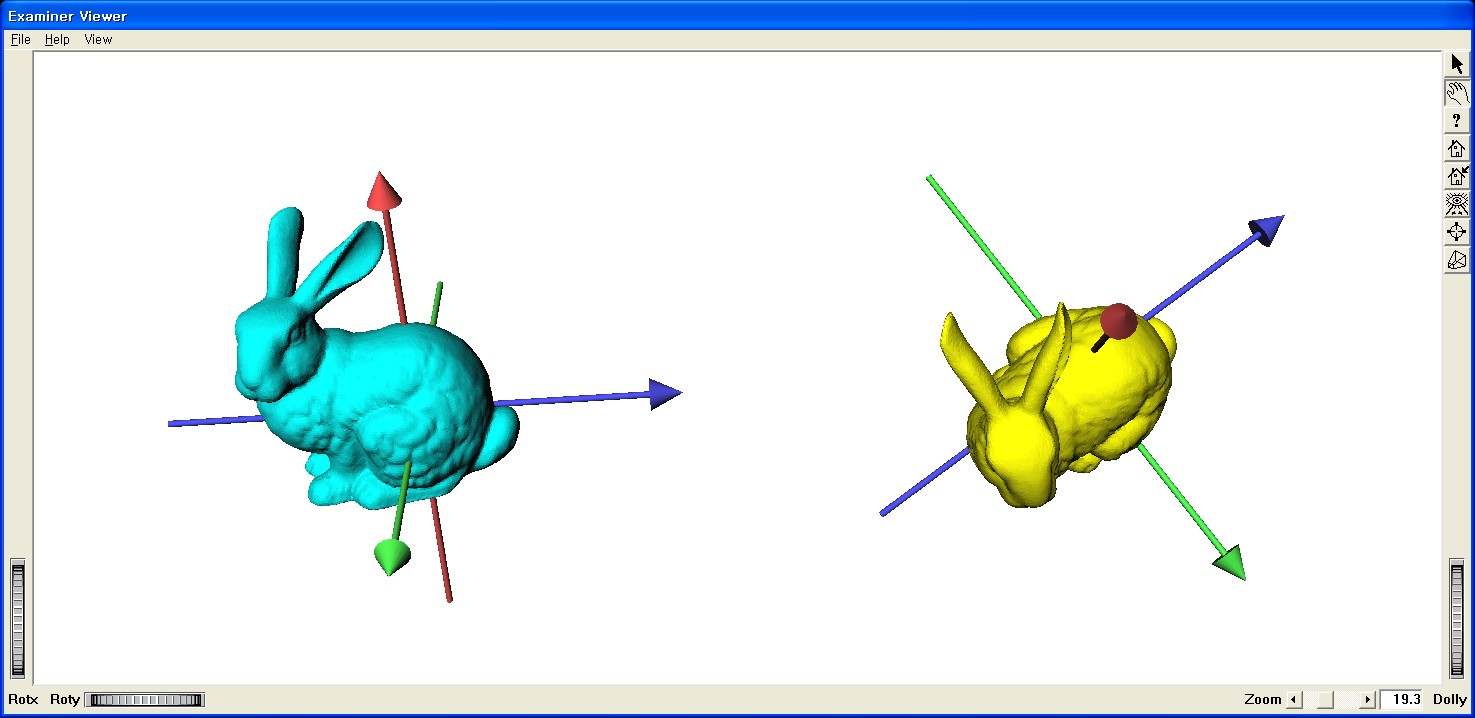
\includegraphics[width=0.45\textwidth]{bunny}
			\caption*{
				\textbf{point} : the 3d location of the bunny \\
				\textbf{vector} : translational movement\\
				\textbf{orientation}: the 3d orientation of the bunny\\
				\textbf{rotation} : circular movement
			}
		\end{SCfigure}
		
	\subsection{Teorema della rotazione di Eulero}
		The general displacement of a rigid body with
		one point fixed is a rotation about some axis.
		
		\noindent
		Qualsiasi rotazione si può esprimere come rotazione di un
		angolo rispetto a un asse.
		
		\noindent
		Qualsiasi rotazione lascia invariati un vettore invariato (l'asse).
		
		\noindent
		Una rotazione qualsiasi rispetto ad un asse passante per
		l'origine puo essere decomposta nel prodotto di tre rotazioni
		rispetto agli assi coordinati; i tre angoli prendono il nome di
		\textbf{angoli di Eulero}.
		
		\noindent
		La rappresentazione con gli angoli di Eulero non è univoca, a
		terne diverse può corrispondere la stessa trasformazione.\\
		Una delle rappresentazioni di Eulero impiega gli angoli roll (rollio),
		pitch (beccheggio) e yaw (imbardata), di derivazione aeronautica.
		
	\subsection{Problemi con angoli Eulero}
			Ci sono alcuni problemi con le rappresentazioni
			delle rotazioni
			\begin{itemize}
				\item Angoli di Eulero:
					Rotazioni non univoche:
					\[
						(z, x, y) [roll, yaw, pitch] = (90, 45, 45) = (45, 0, -45)
					\]
					mandano entrambi l'asse x in direzione $ (1, 1, 1) $
				\item Gimbal Lock (blocco del giroscopio)
				\begin{itemize}
					\item Gimbal è un dispositivo meccanico usato per
				supportare giroscopi o bussole
					\item Ci sono configurazioni problematiche
				\end{itemize}
				\item Interpolazione di rotazioni: Come calcoliamo il punto medio di una rotazione?
			\end{itemize}
	\subsection{Rotazione asse angolo}
		La rotazione generica asse angolo con asse r si può anche
		rappresentare con la seguente matrice, dove 
		$ c = \cos(\alpha) $ e $ s = \sin(\alpha) $:
		\[
			R(\alpha,\vec{r}) =
			\begin{pmatrix}
				(1-c)r^2_1 + c & (1-c)r_1 r_2 -s r_3 & (1-c) r_1 r_2 + s r_2 & 0 \\
				(1-c)r_1 r_2 + s r_3  & (1-c)r^2_2 +c & (1-c)r_2 r_2 -s r_1 & 0 \\
				(1-c)r_1 r_3 -sr_2 & (1-c) r_2 r_3 + s r_1 & (1-c)r^2_3 +c & 0 \\
				0 & 0 & 0 & 1 
			\end{pmatrix}
		\]
	\subsection{Matrici e proiezioni}
		\begin{enumerate}[label=\textbullet]
			\item Abbiamo il nostro mondo dove creare la scena inserendo i
		modelli: spazio Euclideo.
			\item Sappiamo trasformare i punti dello spazio traslando, ruotando
		e scalando.
			\item Per simulare la formazione delle immagini ci serve un ultimo
		strumento geometrico: la modellazione della proiezione degli
		oggetti sul piano immagine.
			\item Questo si fa con la proiezione prospettica o, in casi
		semplificati, con la proiezione ortografica o parallela
			\item Anche queste si possono modellare con matrici, solo che
		dovranno trasformare uno spazio 3D in uno 2D (espressi in
		coordinate omogenee). Quindi sono matrici.
		\end{enumerate}
	\subsection{La macchina fotografica virtuale}
		La metafora utilizzata per descrivere le relazioni
		scena/osservatore è quella della macchina fotografica virtuale
		(synthetic camera).\\
		Il modello semplice usato anche in Computer Vision è la
		\textbf{telecamera pinhole}.
		\begin{figure}[h!]
			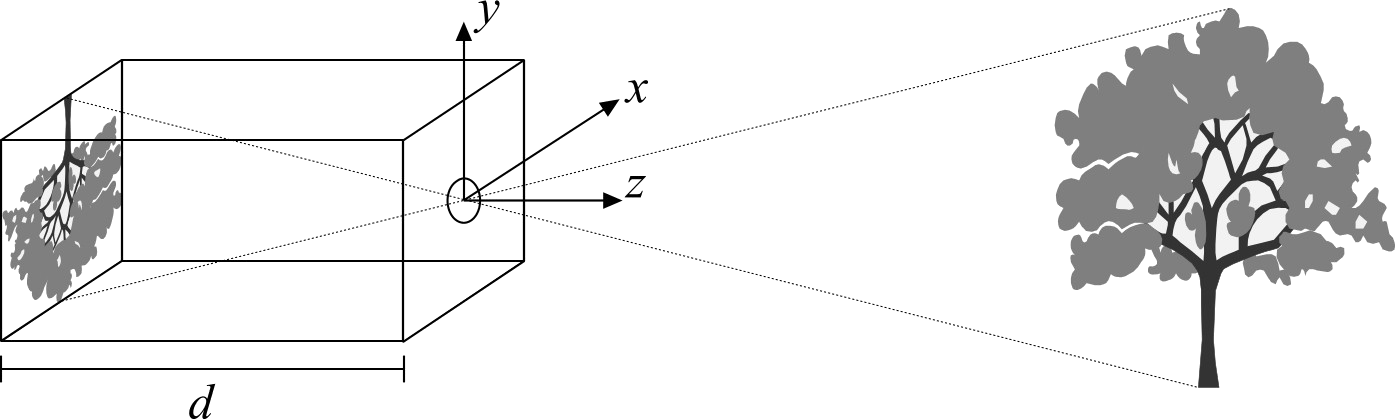
\includegraphics[width=0.5\textwidth]{virtual}
		\end{figure}
		
		La macchina fotografica	virtuale è costituita da un	parallelepipedo in cui la
		faccia anteriore presenta un foro di dimensioni	infinitesime (pinhole
		camera) e sulla faccia posteriore si formano le immagini.
		
		\vspace{-0.5cm}
		\begin{center}
			\begin{tikzpicture}[>=latex]
			\draw[->] (0,-1) -- (0,2) node[right] {$ \vec{y} $};
			\draw[densely dashed] (-3,0) -- (0,0);
			\draw[->] (0,0) -- (3.5,0) node[below] {$ \vec{z} $};
			\draw[densely dashed] (-3,-1) -- (3,1);
			\draw[densely dashed] (-3,1) -- (3,-1);
			\draw (-3,1) rectangle (0,-1);
			\draw[|<->|] (-3.2,1) -- (-3.2,-1) node[midway,left] {$ h $};
			\draw[|<->|] (-3,-1.2) -- (0,-1.2) node[midway,below] {$ d $};
			\draw[densely dashed, bend right] (2.1,-0.7) to (2.1,0.7); 
			\node[right] at (2.3,0.3) {$ \theta $};
			\end{tikzpicture}
		\end{center}
		
		Immagini nitide, nessun	problema di luminosità,	l’angolo di vista può essere modificato variando il rapporto tra la distanza focale (d) e la dimensione
		del piano immagine.\\
		Per convenzione (e maggiore semplicità) si assume l’esistenza
		di un piano immagine tra la scena ed il centro di proiezione \\
		Ne risulta il modello matematico della proiezione prospettica. \\
		
	\subsection{Proiezione prospettica}
		La relazione che lega i punti 3D ai punti sul piano in questa
		ipotesi è data dalla proiezione prospettica. Con semplici
		ragionamenti sui triangoli simili si ha che la proiezione di un
		punto $ P = (P_x, P_y, P_z) $ è data da:
		\begin{itemize}
			\item  $ P' = (-\dfrac{P_x d}{P_z}, -\dfrac{P_y d}{P_z}, 1) $ per il piano immagine dietro.
			\item $ P' = (\dfrac{P_x d}{P_z}, \dfrac{P_y d}{P_z}, 1) $, per il piano immagine davanti.
		\end{itemize}
		Possiamo scrivere la proiezione in forma matriciale:
		\[
			\vec{P'} =
			\begin{pmatrix}
				1 & 0 & 0 & 0 \\
				0 & 1 & 0 & 0 \\
				0 & 0 & 1/d & 1 
			\end{pmatrix}
			\begin{pmatrix}
				P_x \\
				P_y \\
				P_z \\
				1
			\end{pmatrix}
		\]
		
		Da un punto di vista geometrico, la proiezione è
		definita per mezzo di un insieme di rette di proiezione
		(i proiettori) aventi origine comune in un centro di
		proiezione, passanti per tutti i punti dell’oggetto da
		proiettare ed intersecanti un piano di proiezione.
		
		\noindent
		La proiezione di un segmento è a sua volta un
		segmento. Non è quindi necessario calcolare i proiettori di tutti i
		punti di una scena, ma solo quelli relativi ai vertici delle
		primitive che la descrivono.
		
		\noindent
		Le proiezioni geometriche piane si classificano in:
		\begin{itemize}
			\item Proiezioni \textbf{prospettiche} (distanza finita tra il centro ed il piano di
		proiezione)
			\item Proiezioni \textbf{parallele} (distanza infinita tra il centro ed il piano di
		proiezione)
		\end{itemize}
		\begin{figure}[h!]
			\centering
			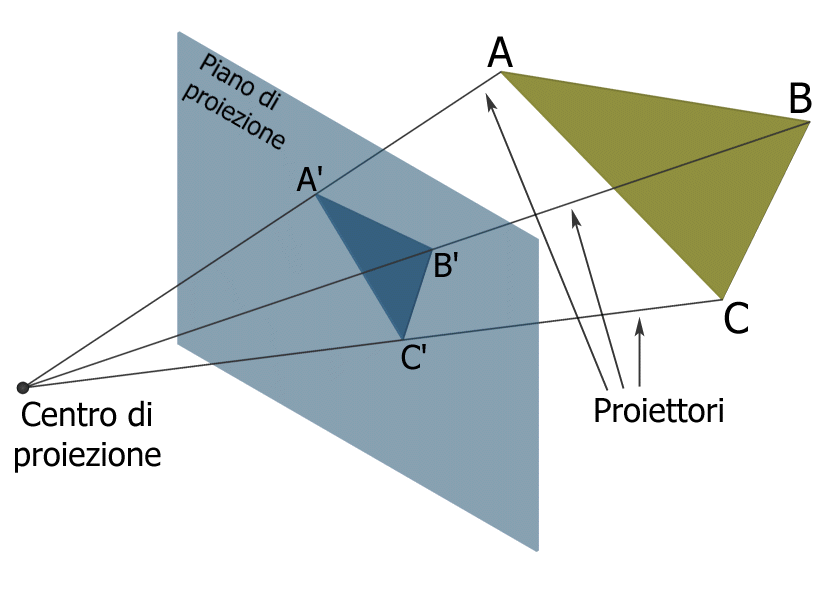
\includegraphics[width=0.4\textwidth]{proiez}
			\hspace{0.2cm}
			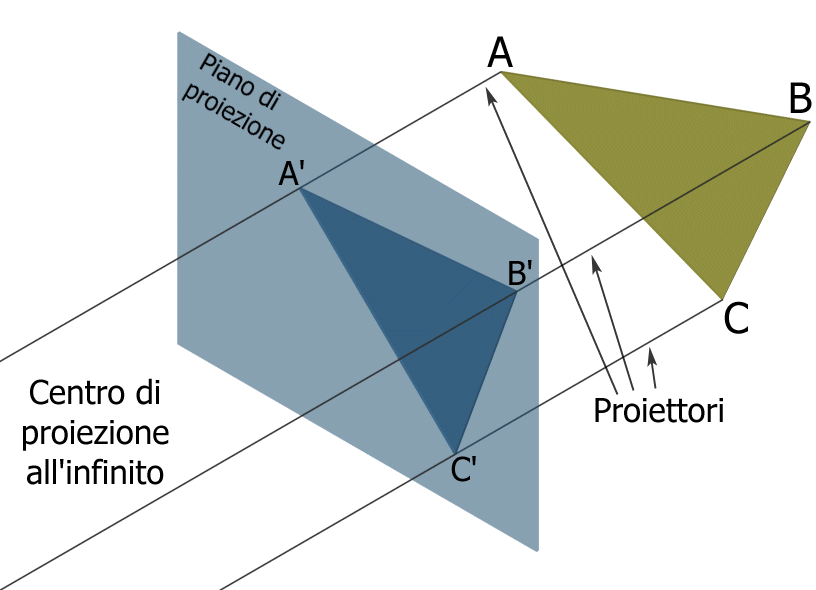
\includegraphics[width=0.4\textwidth]{proiez1}
		\end{figure}
		Al variare della distanza focale $ d $ si ha che:
		\begin{figure}[h!]
			\centering
			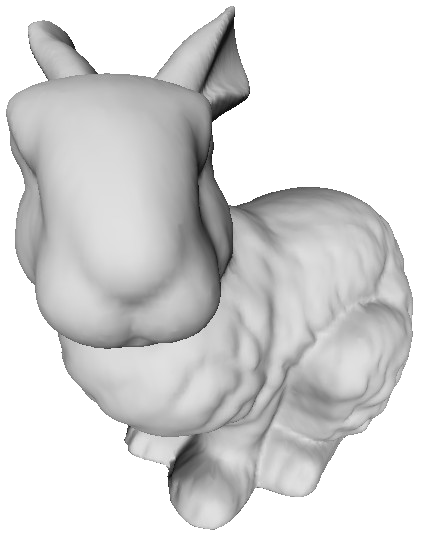
\includegraphics[width=0.13\textwidth]{proiez2}
			\hspace{0.2cm}
			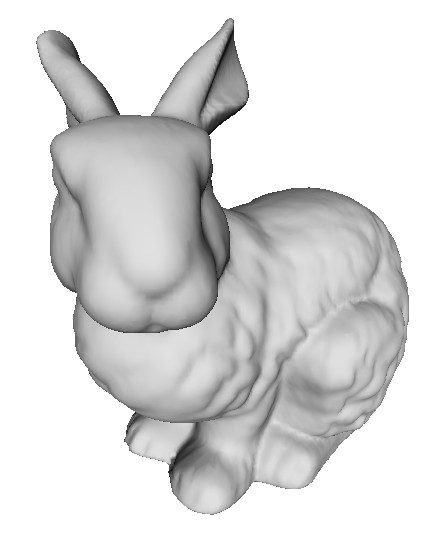
\includegraphics[width=0.15\textwidth]{proiez3}
			\hspace{0.2cm}
			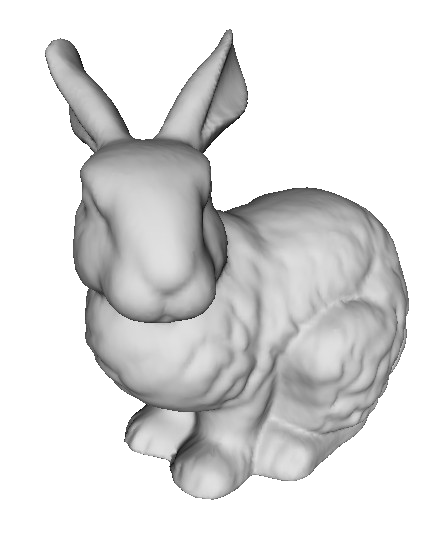
\includegraphics[width=0.15\textwidth]{proiez4}
			\hspace{0.2cm}
			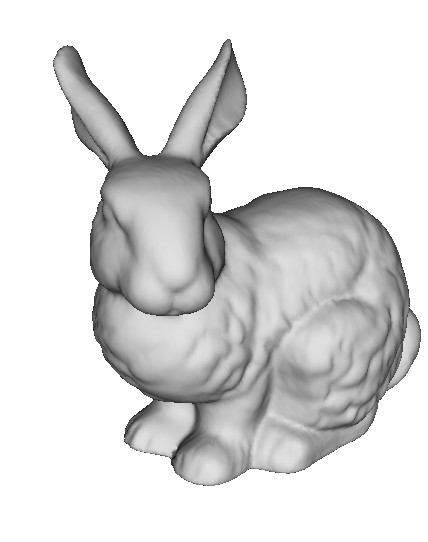
\includegraphics[width=0.15\textwidth]{proiez5}
			\hspace{0.2cm}
			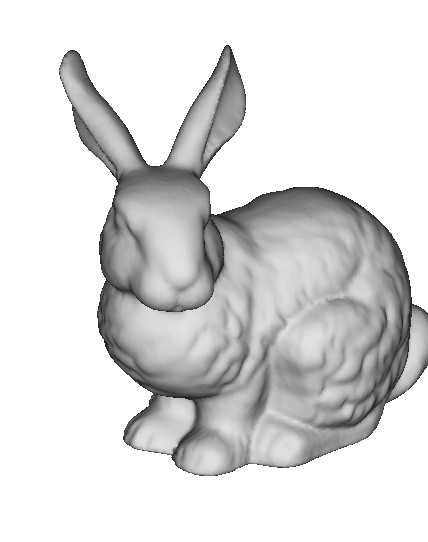
\includegraphics[width=0.15\textwidth]{proiez6}
			
			\begin{tikzpicture}
				\draw[red, thick] (-4,2.5) -- (-4,3) -- (-5,1) -- (-4,-1) -- (-4,-0.5);
				\node[box, draw=red, align = left, ] at (-2.5,1) {
					\footnotesize Più distorsione\\ \footnotesize prospettica\\
					\\
					\footnotesize Effetto "\textit{fish-eye}"\\\footnotesize  (grandangolo)};
				
				\node[box, draw=red, thick, align = left, ] at (2.5,1) {
					\footnotesize Proporzioni\\ \footnotesize più mantenute\\
					\\
					\footnotesize Effetto "\textit{zoom}"\\\footnotesize (es. vista
					dal satellite) };
				
				\draw[red, thick] (4,2.5) -- (4,3) -- (5,1) -- (4,-1) -- (4,-0.5);
				\node at (-5.25,3) {$ d $ piccolo};
				\node at (5.25,3) {$ d $ inifinito};
			\end{tikzpicture}
		\end{figure}
		
		\newpage
		Per motivi che capiremo, in grafica si usa in realtà
		rappresentare la proiezione prospettica con una
		trasformazione che mappa comunque sullo spazio 3D, quindi
		una matrice 4x4.
		
		\noindent
		Per passare alla rappresentazione 2D basta poi eliminare la z
		(che è sempre uguale a $ d $)
		\[
			\vec{P'} =
			\begin{pmatrix}
				1 & 0 & 0 & 0 \\
				0 & 1 & 0 & 0 \\
				0 & 0 & 1 & 0 \\
				0 & 0 & 1/d & 1
			\end{pmatrix}
			\begin{pmatrix}
				P_x \\
				P_y \\
				P_z \\
				1
			\end{pmatrix}
		\]
		In realtà la coordinata omogenea 2D che ricavo 
		dall'applicazione della matrice è 
		\[
			P' = (P_x, P_y ,P_z/d) 
		\]
		L'operazione che trasforma in 
		\[
			P' = (\dfrac{P_x d}{P_z}, \dfrac{P_y d}{P_z} ,1)	
		\]
		per avere la forma standard dei punti è la cosiddetta divisione.\\
		Prima della divisione i tre valori possono essere usati per
		rappresentare l'equivalenza dei diversi punti rispetto alla
		proiezione.
		
		\noindent
		Definiamo ora possibili strutture dati per modellare gli oggetti
		nello spazio.
		
		\noindent
		Poi vedremo come modellare anche la formazione delle
		immagini attraverso il "rendering".
		
\section{Modellare gli oggetti nello spazio}
	\begin{center}
		\begin{tikzpicture}[>=latex, scale=0.8,  every node/.style={scale=0.8}]
		\draw[dashed, rounded corners] (10,-4) rectangle (5,-0.5);
		\node[below] at (7.5, -4) {applicazione interattiva};
		\node[draw, rectangle, rounded corners, align=center] (a) {mondo reale,\\ modello matematico,\\ artista 3D ...};
		\node[draw, rectangle, fill=white, rounded corners, align=center, minimum height=1cm, minimum width=3cm] (b) at (4,-1.5) {Geometria};
		\node[draw, rectangle, rounded corners, align=center, minimum height=1cm, minimum width=3cm] (c)	at (8,-3) {Immagine/i};
		
		\draw[->, rounded corners] (a.east) -- ($ (a) + (4,0) $) node[right,align=left,yshift=0.5cm] {acquisizione 3D (scansione)\\simulazione (elementi finiti)\\modellazione (3DStudioMax, Maya)} -- (b.north);
		\draw[->, rounded corners] (b.south) -- ++(0,-1) -- ++(-3,0) node[below,align=left] {preprocessing\\(modelling)} -- ($ (b) + (-3,0) $) -- (b.west);
		\draw[->, rounded corners] (b.east) -- ($ (c) + (0,1.5) $) node[right] {rendering} -- (c.north);
		\end{tikzpicture}
	\end{center}
	
	\subsection{Geometria Analitica}
	Premessa: prima di vedere come si modellano gli oggetti,
	ricordiamo come si definiscono nello spazio Euclideo 3D le
	figure geometriche importanti dal punto di vista della
	modellazione grafica e del rendering.
	
	\noindent
	\textbf{Rette}: sono identificabili da un punto qualsiasi $ Q $ che giaccia sulla
	retta e da una direzione data da un versore $ u $. È facile vedere che
	sono il luogo dei punti dati da $ P = Q + t\vec{u} \quad t \in \R $\\
	In termini di componenti si vede facilmente che vale la seguente
	equazione 
	\[
		\dfrac{x - x_Q}{u_x} = \dfrac{y - y_Q}{u_y} = \dfrac{z - z_Q}{u_z}
	\]
	 
	Se si vuole specificare una retta dati due punti $ R $ e $ Q $, basta usare le
	formule date qui sopra tenendo conto che il versore che identica la
	retta e dato da: $ \vec{u}=\dfrac{(R-Q)}{|R-Q|} $
	
	\noindent
	\textbf{Semiretta}: basta aggiungere il vincolo $ t \geq 0 $
	
	\noindent
	\textbf{Segmenti}: dati i punti iniziale e finale $ P $ e $ Q $ possiamo scriverli come 
	$ P = Q + t(R-Q) \quad t \in \left[ 0; 1\right]  $
	
	\noindent
	\textbf{Sfere}: dato centro $ O $ e raggio $ r $, i punti della superficie sferica sono dati
	dall'equazione $ P = O + r\vec{u} $ con $ \vec{u} $ versore generico.
	Si dimostra facilmente che, in termini delle coordinate, la
	superficie sferica è data dall'equazione
	\[
		(x - x_0)^2 +(y - y_0)^2 +(z - z_0)^2 = r^2
	\]
	
	\noindent
	\textbf{Piani}: dati 3 punti non allineati $ P $, $ Q $ ed $ R $ il luogo dei punti che descrive
	il piano che li comprende è la combinazione affine
	\[
		S = \alpha P + \beta Q + \gamma R \quad \alpha,\beta, \gamma \in \R \quad \alpha+\beta+\gamma=1
	\]
	Alternativamente si puo definire un piano a partire da un punto $ Q $ che
	vi appartiene e da un vettore $ \vec{u} $ che ne identica la normale come il luogo
	dei punti $ P $ tali che $ (P - Q) \vec{u} = 0 $.
	In termini di coordinate abbiamo
	\[
		(x-x')u_x + (y-y')u_y + (z-z')u_z = 0
	\]
	Per passare dalla prima alla seconda rappresentazione basta
	prendere come punto $ Q $ e come vettore $ \vec{u} = (P-Q) \times (R-Q) $
	
	\noindent
	\textbf{Semispazi}: il piano di cui sopra identica due semispazi, uno
	positivo ed uno negativo:
	\begin{align*}
		(P-Q) \vec{u} &> 0 \\
		(P-Q) \vec{u} &< 0
	\end{align*}
	
	\subsection{Poligoni}
	
	\begin{wrapfloat}{figure}{I}{0pt}
		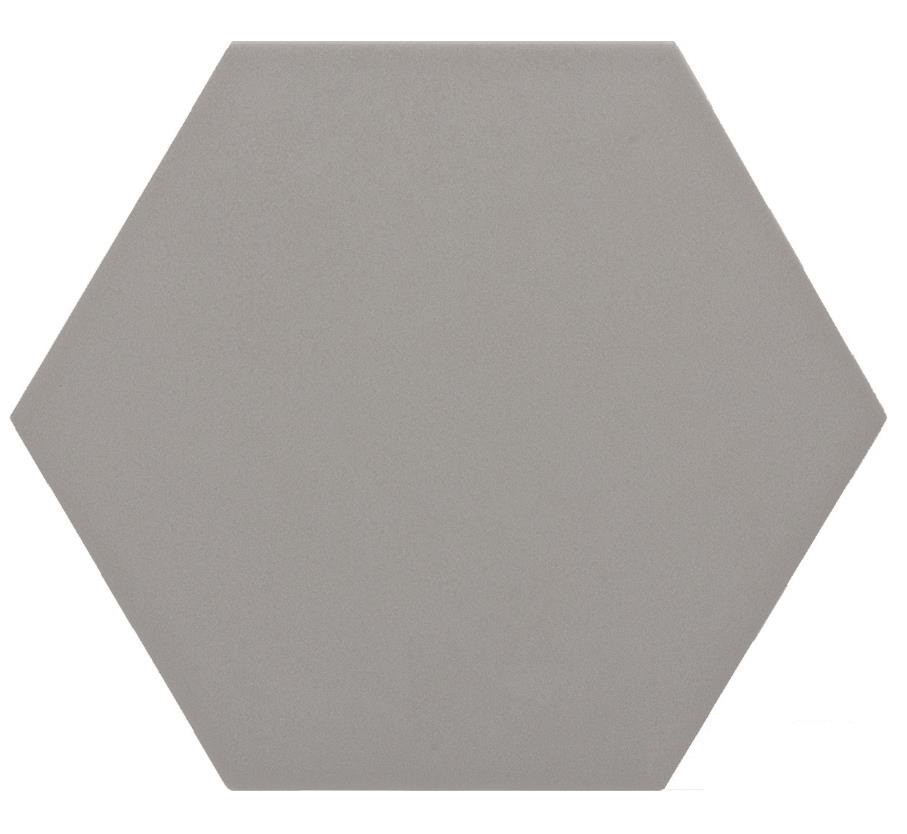
\includegraphics[width=0.2\textwidth]{poligono}
	\end{wrapfloat}
	
		Un poligono $ P $ è un insieme finito di segmenti (spigoli) di $ \R^2 $ , in
		cui ogni estremo (vertice) e comune a esattamente due
		segmenti, che si dicono adiacenti.\\
		Un poligono è detto semplice se ogni coppia di spigoli non
		adiacenti ha intersezione vuota.\\
		\textit{Teorema di Jordan}: Un poligono semplice $ P $ divide il piano in
		due regioni o facce, una limitata (detta interno di $ P $) ed una
		illimitata (detta esterno di $ P $).
		
		\noindent
		Per convenzione, un poligono viene rappresentato dalla
		sequenza dei suoi vertici $ P_1 \dots P_n $ ordinati in modo che l'interno
		del poligono giaccia alla sinistra della retta orientata da $ P_i $ a
		$ P_{i+1} $ , ovvero i vertici sono ordinati in senso antiorario.
		
		\begin{wrapfigure}{R}{0pt}
			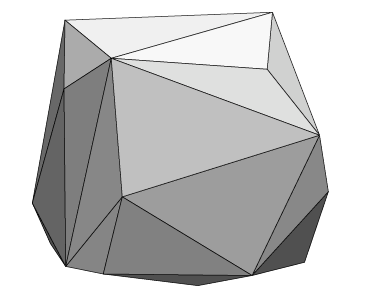
\includegraphics[width=0.2\textwidth, ]{poliedro}
		\end{wrapfigure}
		\noindent
	\subsection{Poliedri}
	
		In $ \R^3 $ un poliedro semplice e denito da un insieme finito di
		poligoni (facce) tali che ciascuno spigolo di una faccia e condiviso
		da esattamente un'altra faccia e le facce non si intersecano che
		negli spigoli.
		
	\subsection{Rappresentazione degli oggetti}
		Gli oggetti che si vogliono rappresentare in una applicazione
		grafica hanno di solito caratteristiche particolari
		\begin{itemize}
			\item Sono finiti
			\item Sono chiusi (non sempre)
			\item Sono continui
		\end{itemize}
		Le rappresentazioni di oggetti (regioni dello spazio, in
		generale) si suddividono in
		\begin{itemize}
			\item basate sul \textbf{contorno} (boundary): descrivono una regione in
		termini della superficie che a delimita (boundary representation, o
		b-rep).
			\item basate sullo \textbf{spazio occupato} (o volumetriche).
		\end{itemize}
		
		\newpage
		La rappresentazione più comune è quella di \textbf{maglie(mesh) di triangoli}:
		
		\begin{tikzpicture}[>=latex, scale=0.8,  every node/.style={scale=0.8}]
			\draw[->] (1,-1) -- (1,4) node [right] {x};
			\draw[->] (1,-1) --(4,-3) node [left] {z};
			\draw[->] (1,-1) -- (-5,-3) node [right] {y};
			\draw[ultra thick, fill=blue] (2.5,-1) -- (0,3) -- (-3,-1.5) -- cycle;
			\fill (0,3) circle (4pt) (a)
				(2.5,-1) circle (4pt) (b)
				(-3,-1.5) circle (4pt) (c);
			\node[yshift=0.2cm,above] at (0,3) {$v_0 = (x_0, y_0, z_0) $};
			\node[xshift=0.2cm,right] at (2.5,-1) {$v_1 = (x_1, y_1, z_1) $};
			\node[xshift=-0.2cm,left] at (-3,-1.5) {$v_2 = (x_2, y_2, z_2) $};
		\end{tikzpicture}
		
		\noindent
		Esistono però delle alternative:
		\begin{itemize}
			\item \textbf{Boundary}:
			Superfici parametriche (lisce, non hanno problemi di "tessellazione"
			cioè visibilità degli spigoli tra le facce)
			\item \textbf{Volumetriche}: 
			\begin{itemize}
				\item Rappresentazione "voxellizata" (a cubetti)
				\item Geometria costruttiva solida
			\end{itemize}
			\item \textbf{Image based rendering}:
			\begin{itemize}
				\item Non si modella effettivamente la scena, ma si memorizzano
				campionamenti della luce, renedendo però possibile una
				visualizzazione da più punti di vista, interattiva
				\item Light fields
			\end{itemize}
		\end{itemize}
		
		Il vantaggio principale nell’uso di superfici per modellare un
		oggetto sarebbe l’assenza del problema della tessellazione
		visibile (cioè approssimo una superficie lisca coi triangoli, ma
		vedo poi i triangoli evidenti, effetto ridotto di solito con
		trucchi opportuni nel rendering)\\
		L'uso di superfici parametriche risulta pesante per applicazioni in
		tempo reale; per lo più le superfici parametriche utilizzate in fase di modellazione o per
		rendering non interattivo.\\
		Negli ultimi tempi le cose sono cambiate ed oggi cominciano
		ad apparire applicazioni di grafica avanzata che usano superfici
		curve anche in tempo reale.
		
		Esempio: \textbf{curve/superfici di	Bezier}:
		Dati $ N $ punti di controllo la curva la curva passa per il
		primo e l'ultimo e approssima gli altri con una funzione da
		essi dipendente. Con una griglia si generano superfici.
		
		\begin{figure}[h!]
			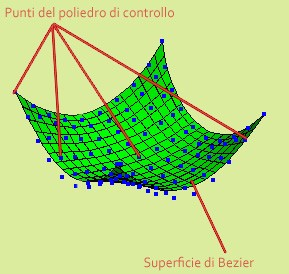
\includegraphics[scale=0.5]{superf}
			\hspace{0.2cm}
			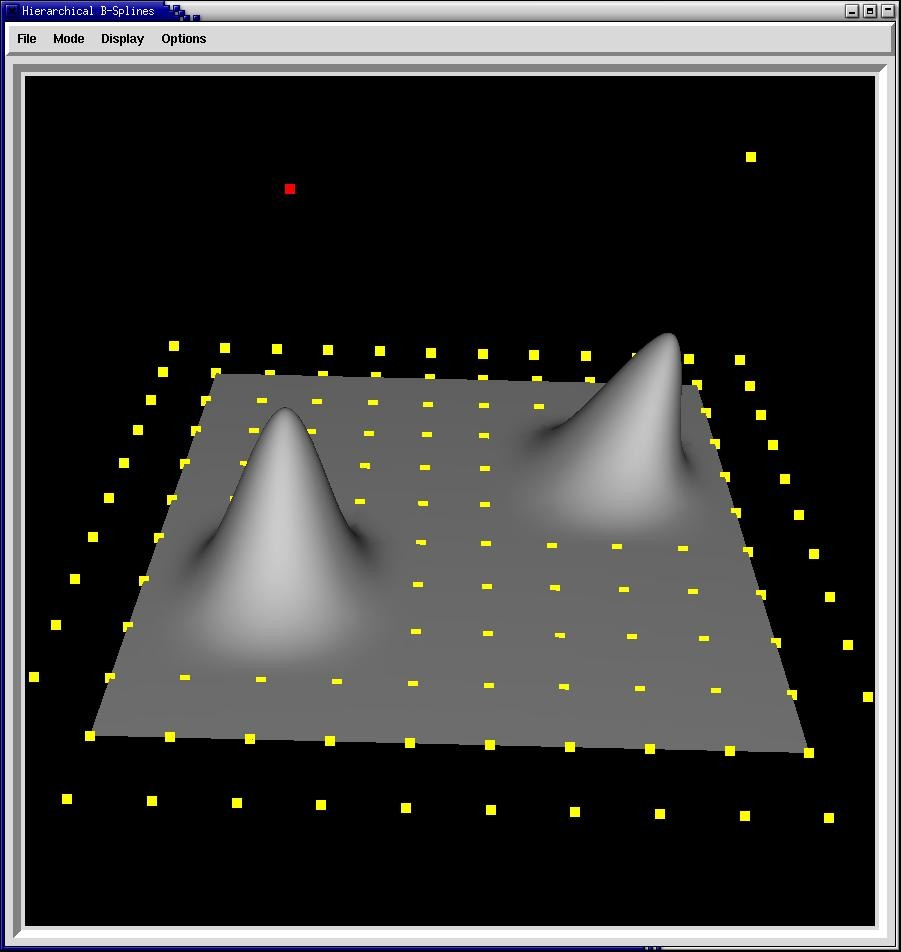
\includegraphics[scale=0.15]{superf1}
			\hspace{0.2cm}
			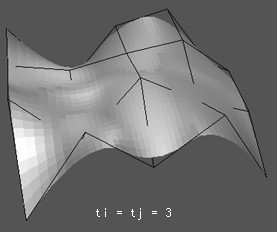
\includegraphics[scale=0.4]{superf2}
		\end{figure}
		
		\subsubsection{Geometria costruttiva solida (CSG)}
		
		Altra rappresentazione particolarmente adatta per il modeling
		(diffusa nel settore CAD), ma poco efficiente per il rendering è quella della
		\textbf{Geometria costruttiva solida (CSG)}.\\
		Si tratta, essenzialmente, di costruire degli oggetti geometrici
		complessi a partire da modelli base con operazioni booleane
		
		\noindent
		\textbf{Operazioni:}
		\begin{itemize}
			\item \textbf{Unione}: l’unione $ A \cup B $ è l’insieme dei punti che appartengono
			ad almeno uno dei due solidi (or non esclusivo).
			\item \textbf{Differenza}: la differenza $ A \setminus B $ è l’insieme dei punti che
			appartengono ad $ A $, ma non a $ B $.
			\item \textbf{Intersezione}: l’intersezione $ A \cap B $ è l’insieme dei punti che
			appartengono ad $ A $ ed a $ B $ (and).
			\item Le operazioni CSG possono essere descritte tramite un albero
			(gerarchia).
			Ciascun nodo di un albero che non sia una foglia contiene una
			delle tre operazioni elementari $ \cup $ , $ \cap $ o $ \setminus $.
			Ciascuna foglia contiene una primitiva.
		\end{itemize}
		
		\subsubsection{Acquisizione dal vero: point clouds}
			Un modo per generare modelli 3D per mondi virtuali è
			acquisire dal vero.\\
			La scansione 3D, oggi tecnologia matura con diverse tecnologie
			Laser, luce strutturata, visione computazionale.\\
			Gli scanner (esattamente come le macchine fotografiche in 2D)
			di fatto non acquisiscono un modello del mondo, ma
			campionano la geometria (con eventuali attributi, es. colore) in
			una serie di punti discreti: si parla di \textbf{nuvole di punti (point
			clouds)}
		
		\subsubsection{Partizionamento spaziale (voxel)}
			Lo spazio viene suddiviso in celle adiacenti dette in 3D voxel
			(equivalente dei pixel delle immagini): una cella è "piena" se
			ha intersezione non vuota con la regione, è detta vuota in
			caso contrario. Oppure contiene un valore di densità (tipico
			dei dati diagnostici es. TAC)\\
			Una rappresentazione di una scena complessa ad alta
			risoluzione richiederebbe l’impiego di un numero enorme
			numero di voxel, per cui questa rappresentazione è in genere
			limitata a singoli oggetti.\\
			Ma le cose stanno cambiando grazie a
			progressi nell'HW e nel SW.\\
			Rendering di modelli voxel-based:
			\begin{itemize}
				\item Algoritmi ad hoc (tecniche direct volume rendering)
				\item conversione da voxel a rappresentazione per superfici (triangle-
				based)
			\end{itemize}
			Da una rappresentazione volumetrica voxelizzata si può
			passare efficientemente a una rappresentazione poligonale
			della superficie mediante l’algoritmo detto marching cubes.
		
		\subsubsection{Rappresentazioni compatte(Octree)}
			Se ho solo i valori pieno/vuoto, posso rappresentare in modo
			compatto il volume con una struttura \textbf{octree}.\\
			Si parte con un cubo contenente la regione e si suddivide
			ricorsivamente. Ci si ferma ogni volta che un ottante contiene
			tutte celle piene o tutte celle vuote.\\
			Più economica rispetto alla enumerazione delle singole celle,
			poiché grandi aree uniformi (piene o vuote) vengono
			rappresentate con una sola foglia (anche se nel caso peggiore
			il numero delle foglie è pari a quello delle celle).

			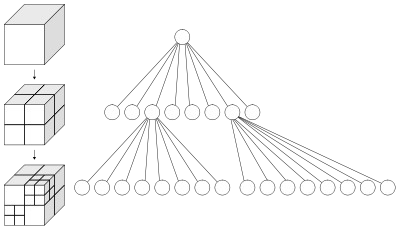
\includegraphics[scale=0.4]{octree}
			\hspace{2.5cm}
			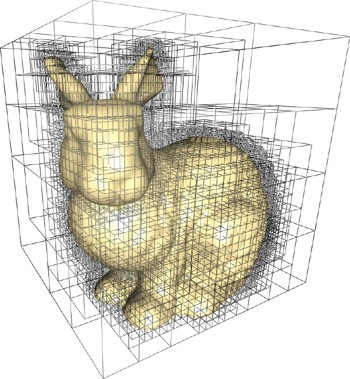
\includegraphics[scale=0.3]{octree2}
			
			Le strutture di partizionamento spaziale sono anche utili per
			"contenere" le geometrie poligonali: come vedremo consente
			di rendere più semplice la ricerca di intersezioni tra oggetti e
			con i raggi ottici.
			
	\subsection{Maglie poligonali (mesh)}
		Nella grafica 3D interattiva si usa quasi sempre la modellazione
		basata su approssimazione poligonale degli oggetti (del loro
		contorno: è una \textit{boundary representation}).\\
		Si tratta di approssimare una superficie 2D con un insieme di
		poligoni convessi opportunamente connessi gli uni agli altri.\\
		Nella pipeline di rendering si lavora in genere con i soli
		\textbf{triangoli}:
		tutte le altre rappresentazioni eventualmente usate nel programma
		sono convertite prima del rendering in triangoli
		Possiamo usare la geometria per definire rigorosamente le
		proprietà dei modelli triangolati.
		
		\bigskip
		\noindent
		Una \textbf{varietà} $k$-dimensionale $ X $ è un sottoinsieme di $ \R^d$  in cui
		ogni punto ha un intorno omeomorfo alla sfera aperta di $ \R^k $.\\
		In generale le superifici degli oggetti solidi (sfere, poliedri, ecc.)
		sono varietà bidimensionali.\\
		\textbf{Omeomorfismo}: applicazione biiettiva, continua, con inversa
		continua. Intuizione: trasformazione senza "strappi".
		In una varietà $k$-dimensionale con bordo ogni punto ha un intorno
		omeomorfo alla sfera aperta o alla semisfera aperta di $ \R^k $ .\\
		Il bordo di $ X $ è l’insieme dei punti che hanno un intorno omeomorfo
		alla semisfera aperta.
		Una varietà è sempre una varietà con bordo, eventualmente vuoto.\\
		Il bordo, se non è vuoto, è a sua volta una varietà $ k-1 $ dimensionale
		senza bordo.
		
		\bigskip
		Una \textbf{maglia (mesh) triangolare} è un'insieme di triangoli le cui
		intersezioni siano esclusivamente vertici e lati (spigoli) dei
		triangoli e che sia anche una varietà bidimensionale con bordo.
		Due triangoli che condividono un lato si dicono adiacenti
		I triangoli della maglia si chiamano anche facce.\\
		La condizione di essere varietà si traduce nei seguenti vincoli
		sulla struttura:
		\begin{itemize}
			\item uno spigolo appartiene al massimo a due triangoli (quelli eventuali
			che appartengono ad uno solo formano il bordo della maglia)
			\item se due triangoli incidono sullo stesso vertice allora devono essere
			raggiungibili l'uno dall'altro attraverso un percorso tra triangoli
			adiacenti ovvero devono formare un ventaglio o un ombrello.
		\end{itemize}
		Si usa il termine condizione 2-manifold (varietà)
		
		\begin{tikzpicture}[ scale=0.3,  every node/.style={scale=0.3}]
			\draw[fill=OliveGreen!90!] (1,0) -- (4.5,-5) -- (5,6) -- cycle;
			\draw[fill=gray!70!] (12,-1) -- (5,6) -- (-5,-3) -- (1,0) -- cycle;
			\draw (1,0) -- (5,6);
			\draw[densely dashed] (4.5,-5) -- (5,6);
			\fill (5,6) circle (10pt) (a)
				(1,0) circle (10pt) (b);
			\draw[ultra thick, red] (5,6) -- (1,0);
			\node[right, xshift=1cm, text =red] at (5,6) {\Huge \textbf{NO}};
		\end{tikzpicture}
		\hspace{2.5cm}
		\begin{tikzpicture}[ scale=0.3,  every node/.style={scale=0.3}]
		\draw[fill=OliveGreen!90!] (1,0) -- (4.5,-5) -- (5,6) -- cycle;
		\draw[fill=gray!70!] (12,-1) -- (5,6) -- (1,0) -- cycle;
		\draw (1,0) -- (5,6);
		\draw[densely dashed] (4.5,-5) -- (5,6);
		\fill (5,6) circle (10pt) (a)
		(1,0) circle (10pt) (b);
		\draw[ultra thick, Green] (5,6) -- (1,0);
		\node[right, xshift=1cm, text =Green] at (5,6) {\Huge \textbf{SI}};
		\end{tikzpicture}
		
		\begin{tikzpicture}[ scale=0.3,  every node/.style={scale=0.3}]
			\draw[fill=TealBlue!30!] (-5,-3) -- (1,0) -- (5,6) -- cycle;
			\draw[fill=TealBlue!30!] (4,0) -- (9,-1) -- (5,6.2) -- cycle;
			\draw[fill=TealBlue!30!] (10,-1.5) -- (5.2,6.3) -- (13,7) -- cycle;
			\node[above, yshift=1cm, text =red] at (5,6) {\Huge \textbf{NO}};
		\end{tikzpicture}
		\hspace{2.5cm}
		\begin{tikzpicture}[ scale=0.3,  every node/.style={scale=0.3}]
			\draw[fill=TealBlue!30!] (-5,-3) -- (1,0) -- (5,6) -- cycle;
			\draw[fill=CornflowerBlue] (1,0) -- (10,-1.5) -- (5,6) -- cycle;
			\draw[fill=TealBlue!30!] (10,-1.5) -- (5,6) -- (13,7) -- cycle;
			\node[above, yshift=1cm, text =Green] at (5,6) {\Huge \textbf{SI}};
		\end{tikzpicture}
		
		Il bordo della maglia consiste di uno o	più anelli (sequenza chiusa di spigoli) o
		loop.\\
		Se non esistono spigoli di bordo la	maglia è chiusa (come quelle che
		rappresentano la superficie di una sfera).\\
		L’\textbf{orientazione} di una faccia è data dall’ordine ciclico (orario o antiorario)
		dei suoi vertici incidenti. L’orientazione determina il fronte ed il retro della
		faccia. La convenzione (usata anche da OpenGL) è che la faccia mostra il fronte.
		
		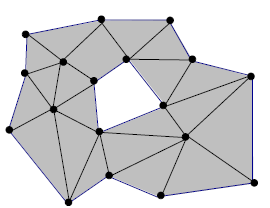
\includegraphics[scale=0.5]{orient}
		\hspace{2.5cm}
		\begin{tikzpicture}[scale=0.5]
			\node[above] at (-3,4) {Fronte};
			\node[above] at (3,4) {Retro};
			\draw[fill=Gray!80!] (-1,0) -- (-3,3) -- (-4,-2) -- cycle;
			\draw (1,0) -- (3,3) -- (4,-2) -- cycle;
			\fill (-1,0) circle (5pt) coordinate [label=below:$V_2$]  (a) 
				(-3,3) circle (5pt) coordinate [label=above:$V_3$] (b)
				(-4,-2) circle (5pt) coordinate [label=below:$V_1$] (c)
				(1,0) circle (5pt) coordinate [label=below:$V_2$] (d)
				(3,3) circle (5pt) coordinate [label=above:$V_3$] (d)
				(4,-2) circle (5pt) coordinate [label=below:$V_1$] (d);
		\end{tikzpicture}
		
		\noindent
		L’orientazione di due facce adiacenti è compatibile se i due
		vertici del loro spigolo in comune sono in ordine inverso. Vuol
		dire che l’orientazione non cambia attraversando lo spigolo in
		comune.\\
		La maglia si dice \textbf{orientabile} se esiste una scelta
		dell’orientazione delle facce che rende compatibili tutte le
		coppie di facce adiacenti.
		
			\begin{figure}[h!]
				\centering
				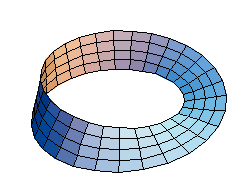
\includegraphics[scale=0.5]{moebius}
				\caption{Non tutte le mesh 2-manifold sono
					orientabili (es. anello di Moebius)} 
			\end{figure}
		
		Abbiamo definito la maglia triangolare. In maniera analoga si
		può estendere la definizione a maglie poligonali generiche\\
		\textbf{Maglie poligonali generiche}: i poligoni possono avere qualsiasi
		numero di spigoli e non è detto che ci sia un solo tipo di poligono.
		Sono raramente utilizzate in grafica al calcolatore\\
		\textbf{Quadrangolari} (quad meshes): gli elementi poligonali sono tutti
		quadrilateri. Sono alle volte usate, per esempio se si vuole fare il
		rendering di un terreno descritto da un array di altezze.\\ In una
		maglia quadrangolare bisogna imporre un vincolo aggiuntivo di
		planarità per ogni quadrilatero che la compone.\\
		OpenGL consente di descrivere maglie poligonali generiche, ma
		per disegnarle li suddivide usualmente in triangoli.
		
	\subsubsection{Equazione di Eulero}
		Se $ V $ è il numero di vertici, $ L $ il numero di spigoli ed $ F $ il numero di
		facce della maglia poligonale orientabile chiusa di genere G, allora
		vale la Formula di Eulero $ V - L + F = 2 - 2G $
		Una superficie ha genere $ G $ se può essere tagliata lungo $ G $
		linee semplici chiuse senza disconnetterla (intuitivamente,
		ma non rigorosamente "numero di buchi").\\
		l genere di una superficie determina la sua
		topologia; per una sfera, per esempio, $ G = 0 $,
		mentre per un toro (una ciambella) $ G = 1 $.\\
		Più in generale, per una maglia poligonale orientabile (e varietà
		bidimensionale) vale la formula $ V - L + F = 2(S - G) - B $\\
		$ S $ numero di componenti connesse, $ B $ è il numero di anelli di bordo.
		
	\subsection{Mesh di triangoli}
		Nella pratica sono il tipo di modello dominante, usato nella gran parte delle applicazioni interattive dato che il rendering è ottimizzato in hardware.\\
		Generate da modellazione CAD, acquisizione con scanner,
		ricostruzione da immagini (Computer Vision).\\
		Il numero di poligoni determina il dettaglio, ma il costo in
		memoria può essere notevole.
		
	\subsection{Costruzione della mesh triangolare}
		Conversione da altri formati:
		\begin{itemize}
			\item Poligoni $ \longrightarrow $ Triangoli
			\item Superf. Quadriche $ \longrightarrow $ Triangoli
			\item Campi di altezze o Punti $ \longrightarrow $ Triangoli
		\end{itemize}
		Per rappresentare gli oggetti con le proprietà fisiche relativa a
		colore e riflessione della luce, devo abbinare alla geometria dei
		valori di proprietà (\textit{attributi})\\
		Posso definirli:
		\begin{itemize}
			\item per vertice: esplicito un attributo per ogni vertice
			\item per faccia: esplicito un attributo per ogni faccia
			\item per wedge (vertice di faccia): esplicito tre attributi per ogni faccia
		\end{itemize}
		Attributi più comuni: Colore, Normali (versori perpendicolari), coordinate texture.\\
		Non è sempre semplice modellare le entità da rappresentare
		con triangoli. Ad esempio: Nuvole, Fiamme, Capelli, pelliccia etc.
		
		\bigskip
		
		Quando si devono disegnare due triangoli con uno spigolo in
		comune, questo viene disegnato due volte. Questo introduce
		un certo grado di ridondanza che può incidere sulle prestazioni.\\
		Si preferisce quindi raggruppare i triangoli di una maglia in
		opportuni gruppi che possono essere elaborati in maniere più
		efficiente. Si possono ad esempio utilizzare:
		\begin{itemize}
			\item \textbf{Fan di triangoli}: è un gruppo di triangoli che hanno in comune un
			vertice. Il primo viene specificato completamente, per i successivi
			basta dare il nuovo vertice. Efficiente, ma i triangoli che incidono su
			un vertice sono in genere pochi.
			\item \textbf{Strip di triangoli}: gruppo di triangoli che posseggono a due a due
			uno spigolo in comune. Di nuovo il primo triangolo viene specificato
			normalmente, per i successivi basta specificare il nuovo vertice.
			Meno efficiente, ma le strip in genere contengono più triangoli delle
			fan.
		\end{itemize}
		Esistono algoritmi per creare queste rappresentazioni dalle
		mesh.
		
	\subsection{Mesh e rendering}
		Per determinare l’effetto di una qualsiasi trasformazione affine
		su un oggetto (traslazione, rotazione, scalatura, composizioni
		varie di queste), basta applicare la trasformazione ai vertici
		(che sono punti); le informazioni connettive date dagli spigoli
		non cambiano in questo tipo di trasformazioni.\\
		Questo rende piuttosto semplice il rendering di oggetti descritti in
		termini di maglie poligonali. Qualsiasi trasformazione viene eseguita
		sui vertici, cioè si tratta di applicare trasformazioni affini su punti.\\
		L’affermazione precedente è vera anche per la proiezione; per vedere
		come si proietta la forma di una maglia su un piano (l’immagine),
		basta seguire la proiezione dei vertici.
		
	\subsection{Memorizzazione}
		Alla creazione dei modelli vengono in genere generati nodi,
		connettività e attributi. Gli algoritmi di processing e rendering
		devono accedere in vario modo a tale informazione.
		Esistono diversi modi di rappresentare questa informazione.\\
		Nei programmi applicativi sono quindi necessarie delle
		procedure per convertire una rappresentazione in un’altra. \\
		Progettare ed implementare tali procedure è un ottimo modo
		per capire nel dettaglio le varie rappresentazioni utilizzate per
		descrivere maglie poligonali.\\
		Nei disegni e negli esempi ci concentreremo sul caso di maglia
		triangolare, ma il discorso è valido in generale per tutti i
		poligoni convessi.
	\subsection{Elementi base}
		\textbf{Vertici}: sono gli elementi 0 dimensionali e sono identificabili
		con punti nello spazio 3D (essenzialmente tre coordinate);
		alle volte può essere utile associare ai vertici altre
		caratteristiche oltre alla posizione (tipo il colore).\\
		\textbf{Spigoli}: sono elementi 1 dimensionali e rappresentano un
		segmento che unisce due vertici. Di solito non contengono
		altre informazioni.\\
		\textbf{Facce}: sono i poligoni bidimensionali, formati da un certo
		numero di spigoli e di vertici (dimostrare che sono in numero
		uguale). I vertici o gli spigoli si usano per identificare la faccia;
		possono contenere altre informazioni (tipo il colore).\\
		\textbf{Normali}: è fondamentale sapere quale è l’esterno della
		superficie e quale l’interno, e qual è l'orientazione locale della
		superficie; a tal scopo si associa spesso ad una maglia
		poligonale anche l’informazione sulla normale uscente.\\
		La normale $ \vec{n} $ ad una faccia è data dal prodotto vettore di due
		suoi spigoli consecutivi non collineari:\\
		Attenzione al verso: la normale è uscente dal fronte della faccia\\
		Per un triangolo $ (V_1 ,V_2 ,V_3 ) $ si ha: $ \vec{n} = (V_3 -V_2)\times(V_1 -V_2 ) $.
		
		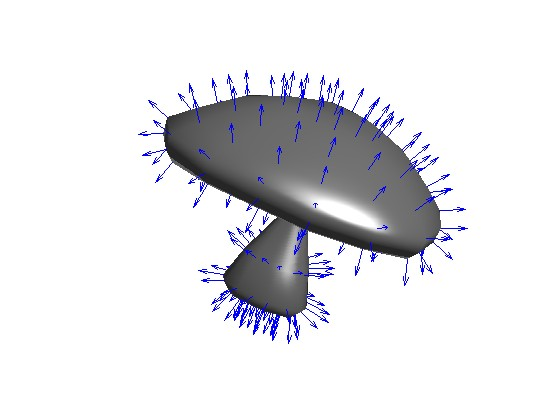
\includegraphics[scale=0.3]{norm}
		
		Attenzione (vedremo in lab): ci servono le normali per
		calcolare il modello di Phong. Le possiamo calcolare per i
		modelli, cui poi sono applicate le trasformazioni geometriche e
		di proiezione.\\
		Ma se applichiamo trasformazioni generiche ai modelli queste
		trasformazioni non preservano necessariamente l'ortogonalità
		di normale e superficie.\\
		Per trasformare senza questo problema le normali possiamo
		trasformarle con una matrice diversa.\\
		Consideriamo un vettore tangente $ \vec{t} $ alla superficie:
		\begin{align*}
			\vec{n}\vec{t}^T &= 0 \\
			\vec{n} M^{-1} M\vec{t} &= 0 \\
			(M^{-1})^T \vec{n} M\vec{t} &= 0
		\end{align*}
		
		Quindi la normale trasformato da $ (M^{-1})^T\vec{n} $ è perpendicolare alla
		superficie trasformata. Cioè per evitare problemi si
		trasformeranno le normali con l'inversa trasposta della matrice
		di trasformazione del modello.
		
	\subsection{Struttura della mesh}
		I vertici danno informazioni di tipo posizionale, gli spigoli
		informazioni di tipo connettivo (non c'è informazione spaziale).\\
		Gli spigoli connettono i vertici, permettendo di introdurre un
		concetto di "vicinanza" tra vertici e dando le informazioni di
		tipo topologico (ovvero definiscono un grafo).\\
		Le facce sono determinate una volta dati i vertici e gli spigoli,
		quindi non introducono nulla.\\
		Al più possono avere associati attributi, anche se è raro.\\
		
		\bigskip
		
		Ci sono vari modi di conservare le informazioni sui modelli.
		Questi possono differire per
		\begin{itemize}
			\item Memoria occupata
			\item Complessità di implementazione di operazioni di ricerca (es. ricerche
			di adiacenza
			\begin{itemize}
				\item Quali sono i vertici vicini a uno dato?
				\item Quali sono gli spigoli che contengono un vertice dato?
				\item Quali sono le facce che contengono uno spigolo?
				\item ...
			\end{itemize}
		\end{itemize}
		Possibilità di controllo sulla qualità delle superfici (es. manifoldness)
		
	\subsection{Lista di triangoli e indexed}
		\begin{itemize}
			\item Immediata: specificare tutte le facce della maglia come
			terne di triplette di coordinate cartesiane
			\item Spreco di memoria: duplico le coordinate. Meglio usare
			una struttura indicizzata, con la lista dei vertici e la
			lista delle facce con i	puntatori ai vertici (indici)
			\item Normalmente usate in openGL per il rendering
			\item Non ottimali per le ricerche
		\end{itemize}
		\begin{multicols}{2}
			\begin{lstlisting}
typedef struct{
	float v1[3];
	float v2[3];
	float v3[3];
} faccia;
			\end{lstlisting}
			\columnbreak
		\begin{lstlisting}
typedef struct {
	float x,y,z;
} vertice;
typedef struct {
	vertice* v1,v2,v3;
} faccia;
		\end{lstlisting}
		\end{multicols}
		
		\begin{figure}[h!]
			\vspace*{-1.2cm}
			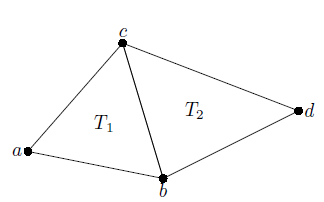
\includegraphics[scale=0.4]{mesh}
		\end{figure}
	
	\subsection{Winged edge (Baugmart 1975)}
		Si aggiungono dei puntatori allo spigolo per
		rendere più semplice l’analisi delle incidenze.\\
		L’elemento base è lo spigolo (edge) con le sue due facce incidenti (wings):
		\begin{itemize}
			\item Lo spigolo $ l_2 $ contiene un puntatore ai due
			vertici su cui incide (b; c), alle due facce su cui
			incide $ (T_1, T_2) $ ed ai due spigoli uscenti da
			ciascun vertice
			\item Un vertice contiene un puntatore ad uno degli
			spigoli che incide su di esso, più le coordinate
			(ed altro)
			\item La faccia contiene un puntatore ad uno degli
			spigoli che vi incide (ed altro).
		\end{itemize}
		La struttura assume che ogni spigolo non di
		bordo abbia due facce incidenti (manifold).
		
		\begin{multicols}{2}
		\begin{lstlisting}
typedef	struct{
	we_vertice* v_ini, v_fin;
	we_spigolo* vi_sin, vi_dstr;
	we_spigolo* vf_sin, vf_dstr;
	we_faccia* f_sin, f_dstr;
} we_spigolo;
typedef struct {
float x, y, z;
	we_spigolo* spigolo;
} we_vertice;
typedef struct {
	we_spigolo* spigolo;
} we_faccia;
		\end{lstlisting}
		
		\columnbreak
		
		\vspace*{1cm}
			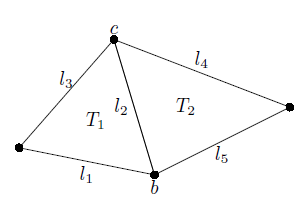
\includegraphics[scale=0.5]{mesh1}
		\end{multicols}
		
	\subsection{Half edge}
		Ogni spigolo viene diviso in due spigoli
		orientati in modo opposto:
		\begin{itemize}
			\item Ciascun mezzo spigolo contiene un puntatore
			al vertice iniziale, alla faccia a cui "appartiene",
			al mezzo spigolo successivo (seguendo
			l’ordinamento) ed al mezzo spigolo gemello
			\item Ogni vertice, oltre alle coordinate (e attributi)
			contiene un puntatore ad uno qualsiasi dei
			mezzi spigoli che esce da tale vertice
			\item Ogni faccia contiene uno dei suoi mezzi spigoli
			(oltre ad altre caratteristiche quali, ad
			esempio, la normale)
		\end{itemize}
		Efficiente per le ricerche ed elegante.
		
		\begin{multicols}{2}		
	\begin{lstlisting}
typedef struct {
	he_vertice* origine;
	he_spigolo* gemello;
	he_faccia* faccia;
	he_spigolo* successivo;
} he_spigolo;
typedef struct {
	float x, y, z;
	he_spigolo* spigolo;
} he_vertice;
typedef struct {
	he_spigolo* spigolo;
} he_faccia;
	\end{lstlisting}
		
		\columnbreak
		
		\vspace*{1cm}
		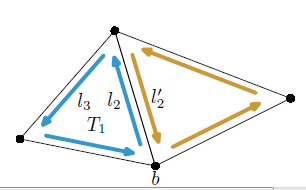
\includegraphics[scale=0.5]{mesh2}
	\end{multicols}
		
	\noindent
	\textbf{Note:}\\
	La stessa applicazione grafica può far uso di più di una
	struttura dati.\\
	La rappresentazione con la lista di vertici essendo semplice e
	leggera è tipicamente usata come formato per i file
	contenenti la geometria di oggetti.\\
	Le applicazioni grafiche in genere caricano tali file ed usano
	l’informazione contenuta in essi per riempire una struttura
	dati più utile ai fini algoritmici (per esempio la half-edge).
	
	
	\section{Rendering}
		Interazione luce-materia.\\
		La luce raggiunge la superficie. Viene riflessa, ma come? Molti
		effetti.\\
		Parte assorbita, parte riemessa, magari in punto diverso visto che
		può essere riflessa sotto la superficie, anche con ritardo di tempo
		Modifica lunghezza d'onda.\\
		Troppo complicato, ma alcuni effetti per essere simulati
		richiederebbero questo. Fosforescenza, fluorescenza, ecc.
		
		\bigskip
		
		\noindent
		In grafica di solito usiamo la \textbf{BRDF} (Bidirectional Reflectance Distribution Function): modelliamo riflessione	come se dipendente da soli 4 parametri.
		Direzione luce incidente-riflessa, è comunque complicatissimo.
		Inoltre assumeremo di poter pensare alla luce come composizione di
		3 fasci monocromatici a frequenze fisse (R,G,B) o di un solo valore di
		luminosità (ovviamente falso).
		
		\noindent
		La radiazione luminosa è caratterizzata da
		\begin{itemize}
			\item distribuzione spettrale, che ne determina il colore
			\item energia che ne determina l'intensità o luminosità
			per ora usiamo in modo informale questi termini.
		\end{itemize}
		\textbf{Fotometria}: la misura dell’energia trasportata dalle
		onde elettromagnetiche della gamma ottica (spettro visibile).
		la fotometria si occupa dell’azione della luce visibile sull’occhio
		umano.\\
		
		\subsection{Radiometria}
		
		\textbf{Radiometria}: si occupa di radiazioni estese sull’intero
		intervallo delle possibili lunghezze d’onda e non considera gli
		effetti sull’osservatore.
		Essendo interessati ad un modello oggettivo, definiremo le
		grandezza radiometriche.\\
		Assumendo che non ci sia interazione tra le diverse lunghezze
		d’onda, si può misurare l’energia indipendentemente per un
		certo numero di lunghezze d’onda campione che servono a
		rappresentare l’intera distribuzione spettrale.\\
		Di solito se ne usano 3, per motivi legati al sistema visivo
		umano, corrispondenti al rosso, verde e blu (RGB).\\
		Tutte le grandezze che definiremo sono implicitamente
		spettrali, ovvero riferite ad una singola lunghezza d’onda.
		
		\bigskip
		
		\noindent
		Le quantità che misuriamo sono:
		\begin{itemize}
			\item Il \textbf{flusso radiante} $ \Phi $ è la velocità alla quale l’energia luminosa viene emessa (o assorbita) da una superficie, ha le dimensioni di una
			potenza (energia per unità di tempo) e si misura in Watt [W].
			\item \textbf{Irradianza} $ E(x) $ il rapporto tra il flusso ricevuto da un elemento
			infinitesimo di superficie in $ x $ e la sua area $ dx $:
			\[
				E(x) = \dfrac{d \Phi}{dx}
			\]
			\item \textbf{Radiosità} $ B(x) $ il rapporto tra il flusso emesso da un elemento
			infinitesimo di superficie in $ x $ e la sua area $ dx $:
			\[
				B(x) =\dfrac{d\Phi}{dx}
			\]
			Irradianza e radiosità sono la stessa grandezza (una densità
			superficiale di flusso) e si misurano in $ \left[ \si{\watt}/\si{\meter}^2 \right] $. La differenza è
			che l’\textbf{irradianza è energia ricevuta}, la \textbf{radiosità è energia
			emessa}. In entrambi i casi, l’energia ricevuta/emessa si considera
			da/verso tutte le direzioni.
			\item L’\textbf{intensità radiante} è il flusso radiante emesso in un angolo
			solido infinitesimo $ d\omega $ lungo una particolare direzione $ \omega $ :
			\[
				I(\omega) = \dfrac{d\Phi}{d\omega}
			\]
			Si usa soprattutto per descrivere sorgenti luminose puntiformi.\\
			\item L’\textbf{angolo solido sotteso} da un oggetto rispetto un punto $ P $ è
			pari all’area della proiezione dell’oggetto su una sfera unitaria
			centrata in $ P $.
			\item L’\textbf{angolo solido sotteso} da un elemento infinitesimo di
			superficie $ dx $ centrato in $ x $ ed orientato con normale $ \vec{n} $,
			rispetto ad un punto $ y $ distante $ r $ vale: $ d\omega = dx \cos\theta/ r_2 $
			dove $ \theta $ è l’angolo formato dalla normale $ \vec{n} $ con la congiungente
			$ y $ ed $ x $.\\
			Il termine $ dx \cos\theta $ rappresenta l’area proiettata di $ dx $ lungo la
			congiungente $ y $ ed $ x $. Se poniamo in $ y $ una sorgente di luce
			puntiforme con intensità radiante $ I $, allora l'irradianza nel punto $ x $ vale:
			\[
				E(x) = \dfrac{d\Phi}{dx} = \dfrac{I\cos\theta}{r_2}
			\]
			\item \textbf{Radianza} $ L(x,\vec{\omega}) $ nel punto $ x $ in una direzione $ \omega $ è la densità superficiale della intensità radiante in $ x $ lungo la direzione 
			$ \vec{\omega} $, considerando l’area della superficie proiettata:
			\[
				L(x,\vec{\omega}) = \dfrac{dI(\omega)}{dx(\vec{\omega}\cdot\vec{n})}
			\]
			L’area proiettata della superficie infinitesima $ dx $
			è l’area della proiezione di $ dx $ (la cui normale è $ \vec{n} $ ) sul
			piano perpendicolare a $ \vec{\omega} $, e vale dunque $ dx(\vec{\omega}\cdot\vec{n}) $.\\
			La direzione $ \vec{\omega} $ è data da due angoli: l’elevazione $ \theta $ (rispetto
			alla normale alla superficie $ \vec{n} $) e l’azimuth $ \phi $(rispetto ad una
			direzione fissata sulla superficie.)\\
			Possiamo dunque scrivere: $ \vec{\omega}\cdot\vec{n} = \cos\theta$.\\
			La radianza $ L(x,\vec{\omega}) $ è la densità di flusso nel punto $ x $ in una direzione $ \vec{\omega} $, misurata rispetto ad una superficie
			infinitesima perpendicolare a $ \vec{\omega} $.\\
			La radianza è pari al il flusso	radiante per unità di angolo
			solido per unità di area proiettata	lungo la direzione di propagazione, e si misura in 
			$ \left[ \si{\watt}/(\si{\meter}^2 \cdot \si{\steradian}) \right] $.
			
			\begin{center}
				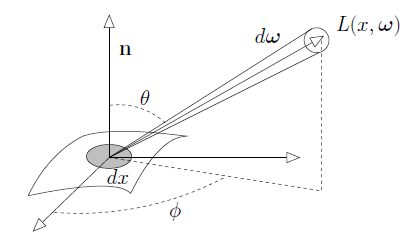
\includegraphics[scale=0.4]{radianza}
			\end{center}
		\end{itemize}
		
		\subsubsection{Radianza lungo un raggio}
			Dati due punti $ x $ e $ y $ (nel vuoto) la radianza che lascia $ x $ verso
			$ y $ è uguale a quella che raggiunge $ y $ dalla direzione di $ x $: non si
			attenua con la distanza.\\
			Il modello che si usa in grafica è quello di raggi luminosi che
			trasportano una certa quantità di energia luminosa.
			Nel ray casting, dunque, i raggi luminosi trasportano radianza,
			ed i pixel registrano il valore della radianza (idealmente).\\
			Quando informalmente si parla di "intensità" del pixel, si fa
			riferimento alla radianza.\\
			In realtà nelle immagini digitali, l'intensità è mappata in un
			range dinamico limitato (tipicamente 8 bit) e non linearmente
			per compensare la non linearità della percezione umana.
			
			Sia $ \Omega $ la semisfera delle direzioni attorno alla normale in $ x $.\\
			Dall'equazione scritta prima si ha:
			\[
				L(x, \vec{\omega})(\vec{\omega}\cdot \vec{n}) = \dfrac{d^2\Phi}{d\vec{\omega}dx} 
			\]
			ed integrando:
			\[
				\int_{\Omega} L(x, \vec{\omega})(\vec{\omega}\cdot \vec{n})d\vec{\omega} =
				\int_{\Omega} \dfrac{d^2\Phi}{d\vec{\omega}dx} d\vec{\omega} =
				\dfrac{d\Phi}{dx} = B(x)
			\]
			Similmente, per l’energia incidente, l’irradianza vale:
			\[
				E(x) = \int_{\Omega} L(x, \vec{\omega})(\vec{\omega}\cdot \vec{n})d\vec{\omega}
			\]
			\textbf{Nota}: la radianza è definita per unità di area proiettata, mentre la
			irradianza/radiosità sono definite per unità di area (effettiva).
			
	\subsection{BRDF}
		Ritroviamo quindi la Bidirectional Reflectance Distribution
		Function (BRDF) che caratterizza il materiale di cui è composta la
		superficie.
		La BRDF $ \rho(x, \vec{\omega_i}, \vec{\omega_r}) $, è il rapporto tra la radianza riflessa da $ x $
		lungo la direzione $ \vec{\omega_r} $ e l'irradianza della luce incidente nel
		punto $ x $ da un angolo solido infinitesimale $ d\vec{\omega_i} $ centrato in $ \vec{\omega_i} $ :
		
		\begin{center}
			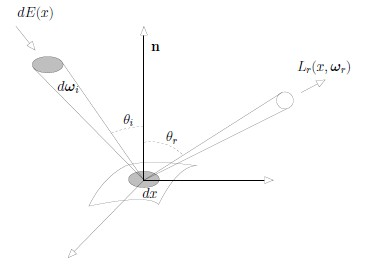
\includegraphics[scale=0.5]{brdf}
		\end{center}
		
		\noindent
		4 gradi di libertà (due angoli). Sarebbero 5 se considerassimo
		la dipendenza dalla lunghezza d'onda della luce.
		E' già una drastica semplificazione.
		Supponiamo che localmente sia costante (stesso materiale in
		una regione).
		Non modella alcuni effetti dei materiali reali:
	\begin{itemize}
		\item Dipendenza dalle lunghezze d'onda.
		\item Fluorescenza: riemissione di energia a frequenze diverse da quelle
		ricevute, tipicamente visibile da stimolo ultravioletto.
		\item Fosforescenza: riemissione anche dopo la cessazione dello stimolo
		Scattering sotto la superficie.
		\item Occorrerebbe, come detto all'inizio, introdurre funzioni con più gradi
		di libertà.
	\end{itemize}
		Si usa la irradianza e non la radianza per misurare la densità di
		flusso incidente perché quest’ultima non tiene conto della
		reale orientazione della superficie.\\
		Si vede facilmente che l'irradianza è legata alla radianza della
		luce incidente $ L_i (x, \vec{\omega_i} ) $ da:
		\[
			dE(x) = L_i (x, \vec{\omega_i} )(\vec{\omega_i} \cdot \vec{n}) d\vec{\omega_i}
		\]
		dove $ P_0 (\vec{\omega_i} \cdot \vec{n}) = \cos\Theta_i $\\
		Dunque la BRDF si scrive :
		\[
			\rho(x, \vec{\omega_i}, \vec{\omega_r}) = 
			\dfrac{L_r (x, \vec{\omega_r})}{L_i (x, \vec{\omega_i} )(\vec{\omega_i} \cdot \vec{n}) d\vec{\omega_i}}
		\]
		Siccome la radianza è definita per unità di area proiettata,
		moltiplicando per $ (\vec{\omega_i} \cdot \vec{n}) $ la si converte in una misura per
		unità di area (non proiettata).\\
		In altri termini, si tiene conto del fatto che la radianza è
		misurata rispetto ad un’area infinitesima orientata
		diversamente da quella che in effetti viene illuminata, mentre
		noi vogliamo esprimere l’effettivo flusso incidente.\\
		Se consideriamo i contributi di irradianza da tutte le direzioni
		di incidenza, la radianza totale riflessa nella direzione $ \vec{\omega}_r $, e
		vale:
		\[
			L_r (x, \vec{\omega}_r) = \int_{\vec{\omega}_i \in \Omega} 
			\rho(x, \vec{\omega_i}, \vec{\omega_r}) L_i (x, \vec{\omega_i} )(\vec{\omega_i} \cdot \vec{n}) d\vec{\omega_i}
		\]
		
		\subsubsection{Diffusione pura}
			Una superficie Lambertiana (o diffusore perfetto) ha una BRDF
			costante: $ \rho(x, \vec{\omega_i}, \vec{\omega_r}) = \rho(x) $. 
			La radianza (riflessa) di tale superficie non dipende dalla direzione.
			Inoltre:
			\begin{align*}
				L_r (x, \vec{\omega_r}) &= \rho(x) \int_{\Omega} L_i (x, \vec{\omega_i} )(\vec{\omega_i} \cdot \vec{n}) d\vec{\omega_i} =
				\rho(x)E(x) = L(x) \\
				B(x) &= \int_{\Omega} L (x, \vec{\omega} )(\vec{\omega} \cdot \vec{n}) d\vec{\omega} = L(x) \int_{\Omega} \cos\theta d\vec{\omega} = \rho(x) E(x)\pi
			\end{align*}
			$ \rho_d(x)= \pi \rho(x) $ prende il nome di \textbf{albedo}.
			\begin{itemize}
				\item L’albedo è la frazione di irradianza $ E(x) $ che viene riflessa come
				radiosità $ B(x) $. Il resto dell’energia viene assorbito
				\item Diffusore perfetto: superficie ruvida (es. gesso, coccio) che ripartisce
				la radianza entrante uniformemente su tutte le direzioni
			\end{itemize}
			
			\bigskip
			
			La specifica esatta della BRDF per superfici reali è estremamente
			difficile da ottenere.\\
			Nella grafica al calcolatore si usano approssimazioni della
			BRDF. Le due più semplici e più usate modellano due
			comportamenti ideali dei materiali: una è appunto la
			diffusione, l'altra è la riflessione speculare.\\
			Un riflettore speculare si comporta come uno specchio
			perfetto, che riflette il raggio incidente lungo una direzione
			che forma con la normale lo	stesso angolo formato dalla
			direzione di incidenza.
			\begin{center}
				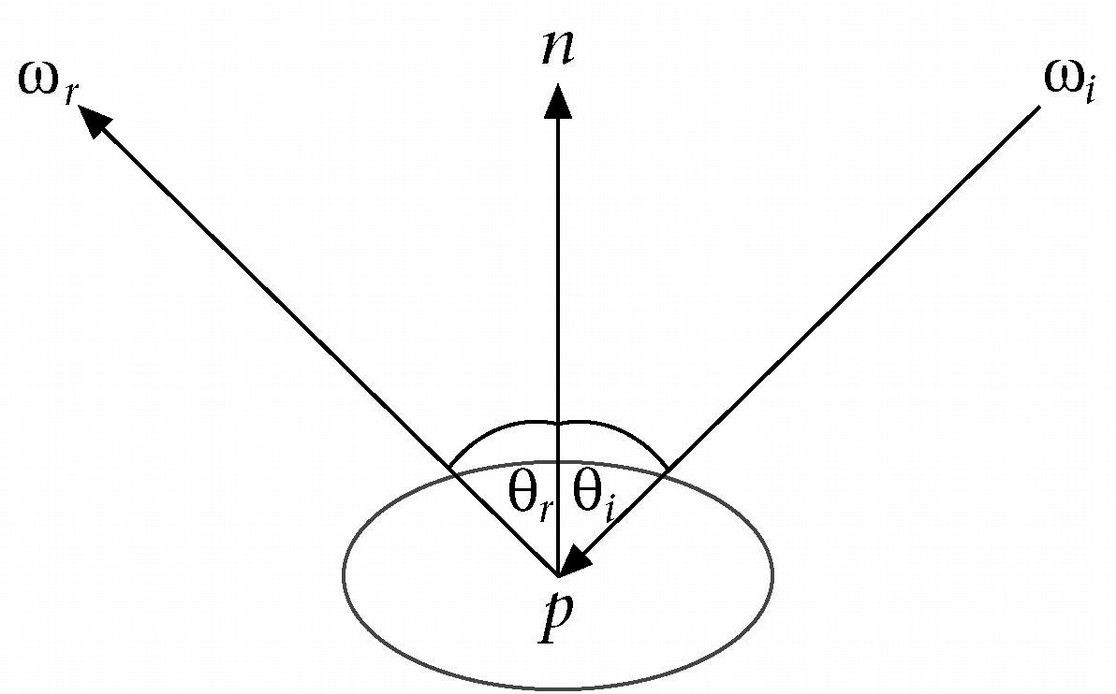
\includegraphics[scale=0.15]{brdf1}
			\end{center}
			
		\subsubsection{Diffusione e riflessione speculare}
			In un materiale opaco (diffusivo) la luce viene riflessa in modo uniforme
			in tutte le direzioni. \\
			In un materiale lucido (glossy) il raggio incidente viene disperso in un cono attorno alla direzione di riflessione perfetta.\\
			Tipicamente le BRDF che si usano in Grafica mescolano
			diffusione e riflessione speculare.\\
			Abbiamo omesso la dipendenza dalla lunghezza d’onda, ma la
			BRDF, in generale, dipende anche da essa: le superfici appaiono
			colorate per questo: la luce bianca (spettro uniforme) incide
			sulla superficie e grazie all’assorbimento selettivo delle
			componenti cromatiche la luce riflessa ha una distribuzione
			spettrale non uniforme, ovvero è "colorata".\\
		
	\subsection{Equazione del rendering}
		La radianza riflessa in direzione $ \vec{\omega}_r $ , dovuta all'irradianza lungo
		una direzione $ \vec{\omega_i} $ è:
		\[
			L_r(x, \vec{\omega_r}) = \rho(x,\vec{\omega}_i, \vec{\omega}_r)L_i (x, \vec{\omega_i} )(\vec{\omega_i} \cdot \vec{n})
		\]
		La radianza totale riflessa lungo $ \vec{\omega}_r $ , è la somma dei contributi
		dovuti a tutte le possibili direzioni incidenti, $ \theta $, quindi vale:
		\[
			L_r(x, \vec{\omega_r}) = \int_{\Omega} \rho(x, \vec{\omega_i}, \vec{\omega_r}) 
			L_i (x, \vec{\omega_i} )(\vec{\omega_i} \cdot \vec{n}) d\vec{\omega_i}
		\]
		
		Aggiungendo la radianza emessa $ L $ e $ (x, \vec{\omega}) $ si ottiene l'
		\textbf{equazione del rendering, o della radianza} (Kaijya, 1987), che
		esprime la radianza totale che lascia il punto $ x $ nella direzione $ \vec{\omega} $:
		\[
			\boxed{L(x, \vec{\omega}) = L_e(x, \vec{\omega}) = 
			 \int_{\Omega} \rho(x, \vec{\omega_i}, \vec{\omega_r}) 
			L_i (x, \vec{\omega_i} )(\vec{\omega_i} \cdot \vec{n}) d\vec{\omega_i}}
		\]
		La radianza incidente in $ x $ lungo la direzione 
		$ \vec{\omega}_i , L_i (x, \vec{\omega}_i) $ è uguale alla radianza emessa da un altro punto $ y $ nella direzione sotto cui $ y $ vede $ x $: 
		$\: L_i (x, \omega_{xy} )= L_i(x, \omega_{yx} ) $ con $ \omega_i = \omega_{xy} $.\\
		L’angolo solido infinitesimo $ d \vec{\omega} $ sotto cui $ y $ vede $ dx $ vale:
		\[
			d\vec{\omega} = dy \cos\theta_{yx} / \|x-y\|^2
		\]
		Introduciamo il termine di visibilità $ V(x,y) $ che vale 1 se e
		solo se $ x $ è visibile da $ y $. Possiamo quindi trasformare
		l’equazione del rendering da integrale su una semisfera di
		direzioni ad integrale su tutte le superfici $ S $ della scena:
		\[
			L(x, \vec{\omega}) = L_e(x, \vec{\omega}) + \int_{y \in S} \rho(x, \vec{\omega}_{xy}, \vec{\omega}) L(y, \vec{\omega}_{yx}) G(x, y) dy 
		\]
		Il termine $ G(x, y) = \dfrac{\cos\theta_{xy}\cos\theta_{yx}}{\| x-y \|^2}V(x,y) $
		dipende solo dalla geometria della scena.
		
		\bigskip
		\noindent
		Per determinare il colore del pixel nel ray casting dobbiamo risolvere l'equazione del rendering. E' ricorsiva: $ L $ è a sinistra e anche a destra!\\
		La radianza in un punto di una superficie è determinata
		globalmente, poiché dipende non solo dalle sorgenti luminose
		(primarie) ma anche da tutte le altre superfici presenti nell’ambiente
		(sorgenti secondarie): computazionalmente assai oneroso.\\
		La disciplina della grafica al calcolatore è incentrata sulla
		soluzione di questa equazione.\\
		Si propongono soluzioni approssimate, in modo più o meno
		grossolano. Si semplificano sia la BRDF che la ricorsione.\\
		
		\noindent
		Per questo aspetto della ricorsione, i metodi si dividono in locali e globali.
		\begin{itemize}
			\item \textbf{Locali}. Si elimina la ricorsione, tenendo conto solo dell’effetto
			diretto delle sorgenti luminose, trascurando le interriflessioni
			nell’equazione viene considerata la radianza entrante solo lungo le
			direzioni corrispondenti a raggi provenienti direttamente dalle
			sorgenti luminose, la cui radianza è nota (ray casting semplice).
			\item \textbf{Globali}. Si tiene conto della natura ricorsiva della equazione
			della radianza, ma si trascurano alcuni fenomeni di
			interriflessione per rendere il problema trattabile. Esempi:
			\begin{itemize}
				\item ray tracing, corretto solo per le riflessioni speculari
				\item radiosity che modella solo le interriflessioni tra superfici diffusive
			\end{itemize}
		\end{itemize}
		
		
	\subsection{Illuminazione globale e locale}
		Per simulare realmente la fisica della luce:
		\begin{itemize}
			\item Occorre avere un modello locale di riflessione del raggio incidente sul
			materiale.
			\item Occorre modellare le interriflessioni (globale) che fanno sì
			che l'illuminazione di ogni punto dipenda da tutta la scena
		\end{itemize}
		Intanto cerchiamo di definire un modello approssimato di riflessione.
		
		\subsubsection{Modello di Phong}
			Un modello di illuminazione locale tratta l’interazione tra una
			sorgente ed una singola superficie, buttando via del tutto la
			ricorsione.\\
			Nei modelli locali ciascun punto viene trattato
			indipendentemente dal resto della scena (no interriflessioni,
			no ombre, no riflessioni speculari).\\
			Modello di illuminazione: data la normale alla superficie, il
			materiale e la direzione di illuminazione, fornisce il colore
			Il modello di Phong è semplice, abbastanza veloce
			da funzionare in tempo reale e produce risultati accettabili, per
			scene semplici.	Può essere usato come base per realizzare algoritmi di illuminazione
			globale (ray tracing). Può essere usato per il rendering in pipeline di rasterizzazione.
		
			\bigskip
		
			\noindent
			Modello dovuto a Phong Bui-Tran, prima metà degli anni '70.
			Semplifica lo schema fisico di interazione:
			\begin{itemize}
				\item Solo sorgenti puntiformi
				\item Calcolo locale dell’equazione di illuminazione
				\item No inter-riflessioni
				\item Approssimazione con due costanti della funzione di riflessione
				\item Simula il comportamento di materiali opachi
				\item Non modella la rifrazione: no materiali trasparenti o semi-trasparenti
				\item Non considera le ombre proiettate
			\end{itemize}
			Le formule che seguono sono in un’unica banda cromatica:
			servono per la produzione di un’immagine a diversi livelli di
			intensità (toni di grigio) piuttosto che diversi colori.\\
			Quando si utilizza una rappresentazione a colori RGB
			l’equazione viene calcolata in modo indipendente per ciascuna
			delle tre componenti cromatiche.\\
			La luce viene considerata composta da tre componenti
			cromatiche R,G,B. Si calcola l’intensità indipendentemente per
			ogni componente cromatica, ottenendo un colore. 
			Nel seguito faremo riferimento ad una singola componente.\\
			Confondiamo "l’intensità luminosa" $ I $ con la radianza. La $ I $ è il
			valore che viene assegnato al raggio.\\
			Sia P il punto della superficie di cui si vuole calcolare il colore.
			Questo equivale a calcolare l’intensità luminosa $ I_{out} $ lungo la
			direzione $ \vec{v} $ che congiunge $ P $ con il $ COP $.\\
			Modelliamo i comportamenti puramente "speculari" e diffusivi
			dei materiali usando le leggi di Lambert e Fresnel.
			
		\subsubsection{Legge di Lambert}
			Materiali molto opachi (es.	gesso e legno) hanno una
			superficie che, a livello microscopico, ha piccole
			sfaccettature che riflettono la luce in una direzione casuale.\\
			Integrando su scala macroscopica: la luce si riflette
			uniformemente verso tutte le direzioni, con intensità
			proporzionale al rapporto tra la direzione del raggio incidente e
			la normale alla superficie in quel punto.
			
		\subsubsection{Modellazione della riflessione diffusiva}
			Sorgenti luminose puntiformi:
			\begin{itemize}
				\item posizione nella scena
				\item intensità della luce emessa
			\end{itemize}
			
			
			Dipendenza solo dall’angolo tra la direzione della luce vista da $ P $ ,
			ovvero $ \vec{l} $ e la normale in $ P $, che indichiamo con $ \vec{n} $ e supponiamo
			di norma unitaria. $ \cos(\theta) = \vec{l} \cdot \vec{n} $.
			
			\begin{multicols}{2}
				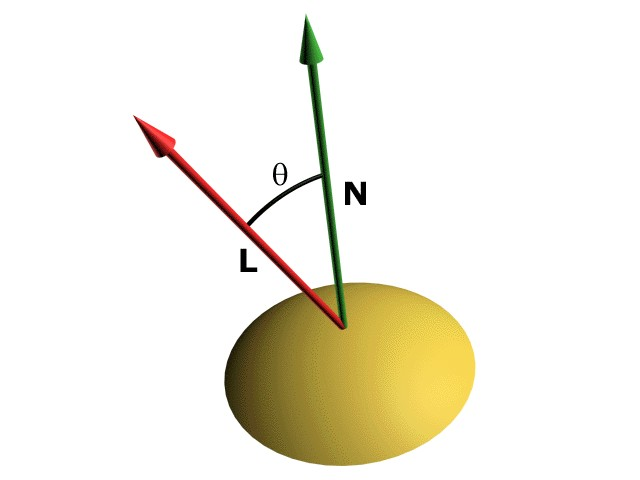
\includegraphics[scale=0.3]{diff}
				
				\columnbreak
				
				\noindent
				Si approssima la funzione di riflessione diffusa della
				superficie come una costante $ k_d $ dipendente dal materiale.\\
				Equazione di illuminazione (solo diffusiva):
				\[
					I_d^{out} = Ik_d\cos\theta = Ik_d(\vec{n}\cdot\vec{l})
				\]
				Simula il comportamento di alcuni materiali (per esempio il
				gesso, o il coccio) i quali riflettono la $ \vec{l} $.
			\end{multicols}
			La componente diffusiva si considera solo per valori di $ \theta $ compresi tra $ 0 $ e $ \pi/2 $.
			
		\subsubsection{Legge di Fresnel}
			\begin{multicols}{2}
				Quando un raggio di luce passa da un mezzo ad un altro con
				diverso indice di rifrazione raggiunta la superficie di
				separazione parte del raggio viene riflessa e parte trasmessa.\\
				La somma delle energie dei due raggi è uguale all’energia del
				raggio originale.\\
				Se da aria a corpo solido non c’è rifrazione si ha solo
				riflessione. L’angolo di incidenza è uguale all’angolo di
				riflessione. Vale per materiali molto lisci e lucidi.
				
				\columnbreak
				
				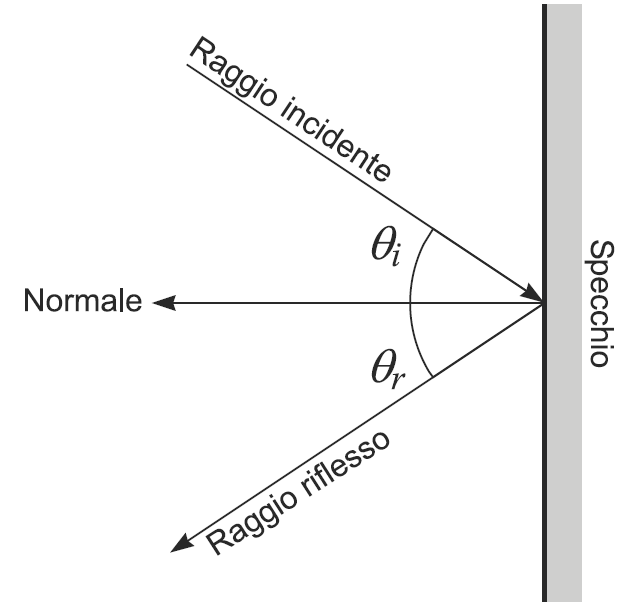
\includegraphics[scale=0.25]{fresnel}
			\end{multicols}
			
		\subsubsection{Modellazione della riflessione speculare}
			Novità sostanziale: riflettore non perfetto\\
			Approssimazione empirica di una riflessione più realistica
			rispetto alla legge di Fresnel.\\
			Conseguenza: \textbf{specular highlight}. Simula superfici lucide in
			generale.
			
			\begin{multicols}{2}
				
				Dipendenza dall’angolo $ \alpha $ compreso tra la direzione di
				riflessione ideale e la direzione di vista.
				Riflessione massima per $ \alpha = 0 $\\
				Decadimento più o meno rapido all’aumentare di $ \alpha $.\\
				
				\columnbreak
				
				\vspace*{-0.8cm}
				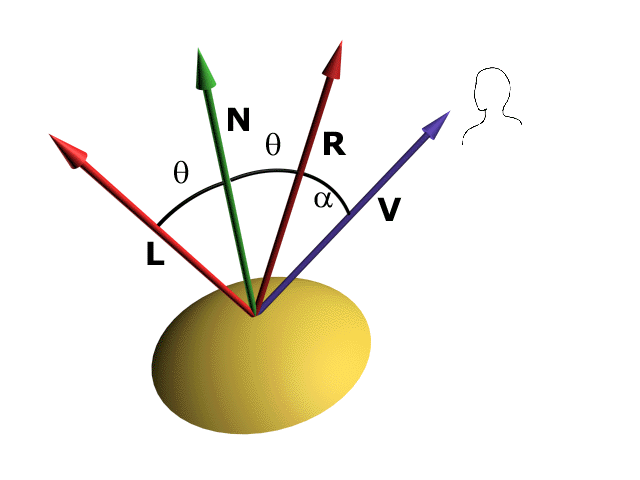
\includegraphics[scale=0.3]{speculare}
				
			\end{multicols}
			Phong (1975) introduce il seguente modello empirico per la
			componente speculare:
			\[
				I_s^{out} = Ik_s (\vec{r}\cdot\vec{v})^n
			\]
			ove $ k_s $ è il \textit{coefficiente di riflessione speculare}
			e $ n $ l’\textit{esponente di riflessione speculare del materiale}.
			$ n $ modula la lucidità della superficie. Per $ n $ che tende ad infinito si ha una
			riflessione speculare perfetta.\\
			La formulazione di Blinn (1977) è leggermente diversa:
			\[
				I_s^{out} = Ik_s(\vec{n}\cdot\vec{h})^n \quad \textup{dove} \quad 
				\vec{h} = \dfrac{1 + \vec{v}}{\| 1+\vec{v} \|}
			\]
			$ H $ è detto "halfway vector", ed è il vettore che biseca
			l’angolo formato da $ \vec{l} $ e $ \vec{v} $.\\
			Il vantaggio della formulazione di Phong-Blinn è che gestisce
			bene il caso in cui l’angolo tra $ r $ e $ v $ sia $ > \pi/2 $.\\
			L’angolo tra $ \vec{n} $ ed $ \vec{h} $ non è lo stesso che c’è tra $ r $ e $ v $: lo
			stesso esponente non produce lo stesso effetto.\\
			Entrambi sono modelli empirici, privi di significato fisico, che
			hanno il merito di simulare credibilmente superfici lucide.
			
			
		\subsubsection{Modellazione della componente ambientale}
			Le inter-riflessioni tra oggetti diversi nella scena non sono
			trattate nel modello di Phong. 
			Effetto parzialmente simulato da una componente "ambientale":
			\[
				I^{out} = I_a k_a
			\]
			\begin{itemize}
				\item $ I_a $ modella la radiazione luminosa totale emessa nella scena. È costante per tutti i punti di tutti gli oggetti.
				\item $ k_a $ modella la rieflettività del materiale.
			\end{itemize}
			La componente ambientale aggiunge realismo alla scena
			
			\begin{center}
				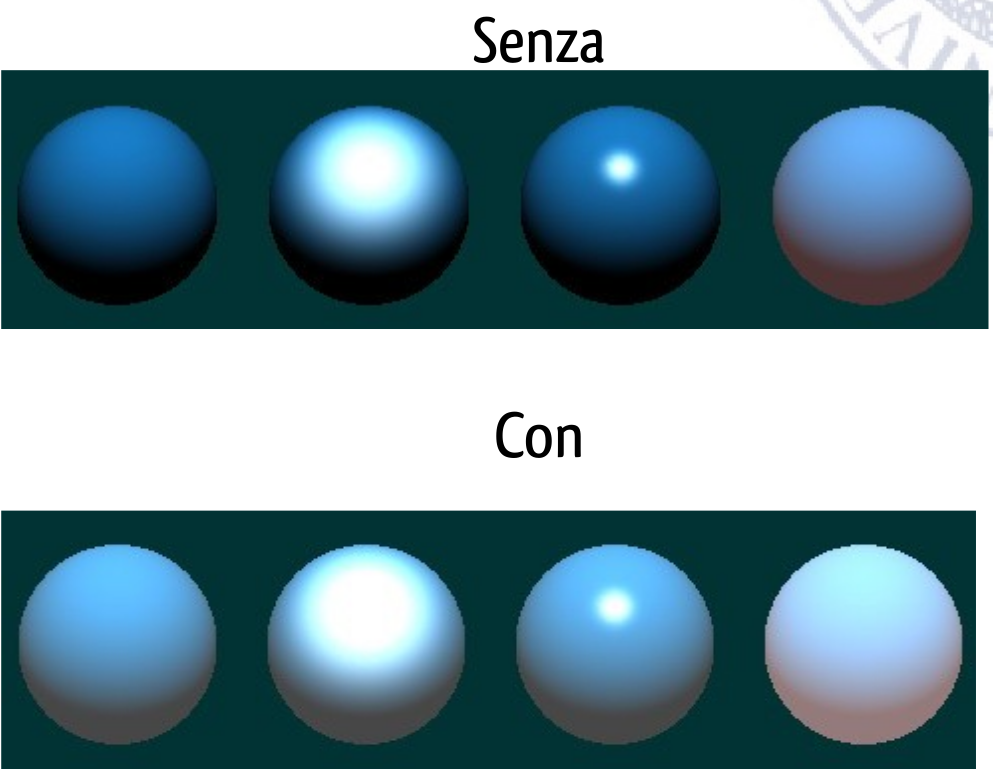
\includegraphics[scale=0.2]{ambientale}
			\end{center}
			Ma da sola non basta!
			
			\bigskip
			
			Tutti i contributi descritti si vanno a sommare per calcolare l’
			illuminazione:
			\[
				I^{out} = I_a k_a + I(k_d(\vec{n}\cdot\vec{l}) + k_s(\vec{n}\cdot\vec{h})^n)
			\]
			Se si stanno considerando i colori, allora sia le intensità della
			luce che i coefficienti del materiale vanno definiti per ogni
			componente (r,g,b):
			\begin{align*}
				I^{r,out} &= I_a^r k_a^r + I^r(k_d^r(\vec{n}\cdot\vec{l}) + k_s^r(\vec{n}\cdot\vec{h})^n) \\
				I^{g,out} &= I_a^r k_a^g + I^g(k_d^g(\vec{n}\cdot\vec{l}) + k_s^g(\vec{n}\cdot\vec{h})^n) \\
				I^{b,out} &= I_a^r k_a^b + I^r(k_d^b(\vec{n}\cdot\vec{l}) + k_s^b(\vec{n}\cdot\vec{h})^n)
			\end{align*}
			
			I coefficienti di diffusione e ambientali di solito sono uguali, la superficie appare del colore specificato dalla terna di coefficienti quando illuminata da luce bianca.
			Le riflessioni speculari (highlights) invece sono di solito del colore
			della luce: $ \quad (k_s^r = k_s^g = k_s^b = 1) $.\\
			
			\textbf{Note:}
			\begin{itemize}
				\item Si parla di modello di Phong, anche se, a rigore, il contributo di Phong
				riguarda il solo termine speculare.
				\item Nella forma più generale, prevede tre componenti separate: luce
				speculare $ I_s $ (riflessa specularmente dalle superfici), luce diffusa $ I_d $
				(diffusa dalle superfici), e luce ambientale $ I_a $
				\item Nella trattazione sopra abbiamo assunto $ I_s =I_d = I $.
				\item Il fatto che una sorgente di luce non emetta luce e basta, ma luce di tre
				tipi diversi non ha un significato fisico, ma può servire a rendere il
				modello più flessibile (per simulare effetti globali). Per esempio, la luce
				ambientale Ia potrà in generale avere un colore diverso dalla $ I $,
				rendendo magari più realistico l’effetto della mutua illuminazione tra le
				superfici: in una stanza con le pareti rosse, la luce ambientale è rossa.
				\item Inoltre, la luce ambientale è associata ad ogni sorgente e non è un
				termine globale unico, così quando una luce viene spenta (o accesa)
				l’illuminazione ambientale diminuisce (o aumenta).
			\end{itemize}
			
	\subsection{BRDF di Phong}
		Vediamo come connettere il modello locale di Phong con
		l’equazione della radianza, per capire che tipo di
		approssimazioni sono state fatte.\\
		Abbiamo introdotto le sorgenti di luce puntuali, che sono
		distinte dagli oggetti della scena, dunque per tutte le superfici
		della scena $ L_e = 0 $.\\
		Per determinare la "intensità" di un punto si deve calcolarne la
		radianza uscente nella direzione $ \vec{\omega} $ che lo unisce al COP:\\
		Dobbiamo quindi calcolare:
		\[
			L(x, \vec{\omega}) = \int_{\Omega}  L(x, \vec{\omega}_i) 
			\rho(x, \vec{\omega}_i, \vec{\omega}) (\vec{\omega}_i\cdot\vec{n}) d\vec{\omega}_i
		\]
		Ma esiste una sola direzione lungo la quale il contributo
		all’integrale è diverso da zero: la direzione $ \vec{\omega}_L $ che punta alla
		sorgente luminosa. Otteniamo dunque:
		\[
			L(x, \vec{\omega}) = L(x, \vec{\omega}_L) \rho(x, \vec{\omega}_L, \vec{\omega})
			(\vec{\omega}_L\cdot\vec{n}) d\vec{\omega}
		\]
		Confrontando con il modello di Phong (senza il termine
		ambientale):
		\[
			I^{out} = I \Big( k_d + k_s\dfrac{(\vec{n}\cdot\vec{h})^n}{\vec{n}\cdot\vec{l}}\Big)
			(\vec{n}\cdot\vec{l})
		\]
		e confondendo la radianza uscente $ L(x, \vec{\omega}) $ con la intensità
		$ I^{out} $ e l'irradianza $ L(x, \vec{\omega}_L )d\vec{\omega} $ con $ I $ si vede che la BRDF di Phong è:
		\[
			\rho(x, \vec{\omega}_i, \vec{\omega}_r) =
			k_d + k_s\dfrac{(\vec{n}\cdot\vec{h})^n}{\vec{n}\cdot\vec{\omega}_i} \quad
			\textup{dove} \quad
			\vec{h} = \dfrac{\vec{\omega}_i + \vec{\omega}_r}{\|\vec{\omega}_i + \vec{\omega}_r\|}
		\]
		Si può associare ad un oggetto una intensità di \textbf{emissione} $ I_e $
		da aggiungere all’intensità calcolata con la formula di Phong.\\
		L’effetto di tale termine è che l’oggetto emette un proprio
		colore oltre alla luce riflessa dalla sorgente luminosa.\\
		Da notare che siccome stiamo lavorando con un modello locale, la luce emessa in questo modo da un oggetto influenza l’apparenza solo di quell’oggetto e non l’apparenza
		degli oggetti vicini (ovviamente poco realistico).\\
		Ovvero: un corpo emissivo non si comporta come una sorgente luminosa, in questo modello locale.
		
		Un modello maggiormente motivato dal punto di vista fisico
		potrebbe essere quello di Cook-Torrance basato sul modello microfacets della superficie, che descrive la superficie come formata da piccole facce disposte in modo
		variabile.
		Il modello di Cook-Torrance differisce da quello di Phong nella
		componente speculare.
		\[
			I_s^{out} = I_s k_s \dfrac{\vec{n}\cdot\vec{l}}{\vec{n}\cdot\vec{v}}FGD
		\]
		dove:
		\begin{itemize}
			\item $ D(\vec{l}, \vec{v}) $ misura la frazione di microfaccette orientate in modo
			da dare riflessione speculare da $ \vec{l} $ a $ \vec{v} $.
			\item $ G(\vec{l}, \vec{v}) $ misura la diminuzione
			di luce riflessa a causa dell’occlusione da parte di altre
			microfaccette.
			\item $ F (\vec{l}, \vec{v}, \lambda) $ è il coefficiente di Fresnel che fornisce la
			frazione di luce incidente che viene riflessa.
		\end{itemize}
		
	\subsection{Ray Casting}
		Dovendo assegnare un colore ad ogni pixel, consideriamo il raggio ottico uscente da ciascun pixel.\\
		Un raggio ottico è una semiretta uscente dal COP che interseca
		il piano vista.
		\begin{itemize}
			\item Se il raggio non interseca alcun oggetto della scena allora gli assegno
			il colore di sfondo.
			\item Se il raggio interseca un oggetto, allora devo calcolare l’illuminazione
			$ I_{out} $ (il colore) nel punto di intersezione ed assegnarlo al pixel.
			\item Per calcolare il colore applico il modello locale (di Phong).
			\item Computazionalmente pesante trovare le intersezioni raggio-oggetti.
			\item Si possono facilmente aggiungere le ombre tracciando il raggio che
			connette il punto d’intersezione con la sorgente luminosa (shadow
			ray ): se esso interseca qualche oggetto allora il punto è in ombra.
		\end{itemize}
		Il calcolo delle intersezioni si può fare con tutti i tipi di primitiva (e di modelli) visti: Sfere, piani, poligoni, poliedri... È computazionalmente pesante, si possono usare strutture dati per semplificare il problema. Es. strutture dati gerarchiche, volumi di contenimento, octrees, kd trees etc.
		
		\bigskip
		
		L’eventuale punto di intersezione tra la retta $ P = Q + t\vec{v} $ ed il
		piano $ (O - P ) \cdot\vec{u} = 0 $ deve soddisfare l’equazione:
		\[
			(O - Q - t\vec{v}) \cdot\vec{u} = 0
		\]
		Dunque si ottiene per $ t_0 $ la seguente soluzione:
		\[
			t_0 = \dfrac{(O - Q) \cdot\vec{u}}{\vec{u}\cdot\vec{v}}
		\]
		che ha senso se $ \vec{u}\cdot\vec{v} = 0 $. Infatti se $ \vec{u}\cdot\vec{v} = 0 $ la retta è parallela al piano (e non lo interseca).
		
		\textbf{Intersezione retta-poligono}:\\
		Per prima cosa si fa un test per vedere se la retta interseca il piano contenente il poligono.
		Quest’ultimo è descrivibile semplicemente da uno dei vertici del poligono e dalla normale a questo. Se la retta non interseca tale piano allora sicuramente non
		interseca nemmeno il poligono. Nel caso di intersezione bisogna determinare se il punto di
		intersezione giace o meno nel poligono. Assumiamo che il poligono P sia convesso. In tal caso un punto $ R $ giace all’interno di $ P $ se e solo se $ R $ si trova nel semipiano
		sinistro di tutte le rette orientate che contengono gli spigoli
		(la retta orientata da $ P_i $ a $ P_{i+1} \quad \forall i = 1 \dots n  $).
		
		[Esercizio: trovare un modo per verificare che $ R $ giace a sinistra della
		retta orientata $ P Q $ ]
		
	\subsubsection{Riduzione della complessità}	
		Implementare un ray-tracer elementare è molto semplice. Basta controllare l’intersezione di ciascun raggio con ogni primitiva (triangolo). Questo ha un costo lineare nel numero delle
		primitive ed è praticabile solo per modelli semplici.\\
		Per raggiungere costo sub-lineare sono necessarie strutture di indicizzazione spaziale, che consentano di limitare a-priori (senza fare il test) il numero delle primitive per le quali il
		test di intersezione viene effettuato.\\
		Queste tecniche di sfoltimento si chiamano anche \textbf{pruning}, culling o broad phase (contrapposto al narrow phase dove invece si calcolano le intersezioni (con test stringenti).\\
		Tipicamente si considerano oggetti convessi. Se non lo sono, si spezzano in parti convesse.
		
	\subsubsection{Volumi di contenimento}
		Si racchiudono gli oggetti in solidi ("volumi") che li
		contengono (bounding volume), con i quali sia facile testare
		l’intersezione: se non c’è intersezione con il bounding volume
		non c’è intersezione con l’oggetto racchiuso.\\
		Questo non rende sub-lineare la complessità della ricerca delle
		intersezioni, ma semplifica le operazioni, e dunque sortisce nella
		pratica un miglioramento dei tempi.\\
		Tipici volumi di contenimento sono sfere, parallelepipedi con i
		lati paralleli agli assi cartesiani (AABB, da axis aligned
		bounding box), oppure parallelepipedi generici (OBB, da
		oriented bounding box).\\
		
		\begin{center}
			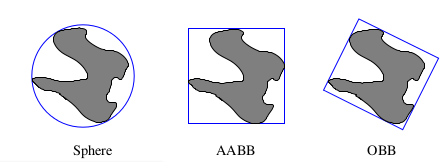
\includegraphics[scale=0.5]{volumi}
		\end{center}
		
	\subsubsection{Partizionamento spaziale}
		Si suddivide lo spazio in celle, tipicamente cubiche (come una
		voxelizzazione grossolana). Si visitano le celle intersecate dal raggio (come Bresenham) e
		solo le primitive contenute in tali celle sono intersecati con il
		raggio.
		
	\subsubsection{Volumi di contenimento gerarchici}
		Si costruisce una gerarchia di volumi di contenimento, dove al livello più alto si ha un volume che racchiude tutta la scene, ed al livello più basso si hanno volumi di contenimento per i singoli oggetti (o per un numero prefissato di primitive). È una struttura organizzata bottom-up. È stata introdotta proprio per il ray tracing.
		
		\begin{center}
			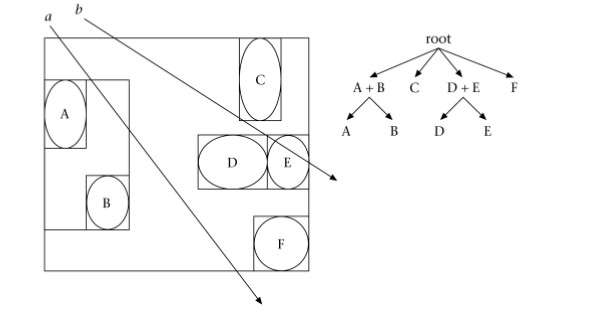
\includegraphics[scale=0.5]{volumiger}
		\end{center}
	
	\subsubsection{Octree}
	La costruzione dell’Octree avviene come di consueto: una cella viene suddivisa ricorsivamente fino a che non contiene un numero prefissato di primitive. L’attraversamento (sequenziale) avviene nel seguente modo:
	\begin{itemize}
		\item Interseca il raggio con il cubo che racchiude tutta la scena (nodo
		radice) e trova un punto P sul raggio “leggermente” all’interno.
		\item Visita l’albero per scoprire a quale cella (foglia) appartiene P .
		\item Interseca il raggio con le facce della cella per trovare la faccia di
		uscita.
		\item La prossima cella è quella adiecente alla faccia di uscita.
	\end{itemize}
	Come nel caso della partizione uniforme, solo le primitive contenute nelle celle visitate sono intersecati con il raggio. Il vantaggio è che la divisione si adatta agli oggetti della scena
	invece di essere fissa ed uniforme.
	
	\begin{center}
		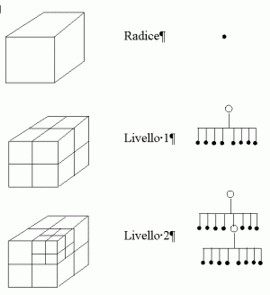
\includegraphics[scale=0.5]{octree3}
		\hspace{1cm}
		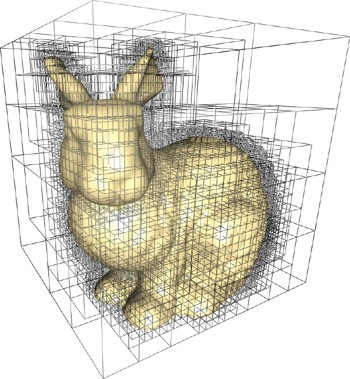
\includegraphics[scale=0.5]{octree2}
	\end{center}

	\subsubsection{KD-Tree}
	La costruzione avviene in modo che ogni piano divida a metà il numero di oggetti rimanenti. L’attraversamento può avvenire in modo sequenziale (come quello visto per l’Octree) oppure in modo ricorsivo, sfruttando la struttura dell’albero. Vediamo quest’ultimo:
	\begin{quote}
		Il raggio viene intersecato ricorsivamente con le regioni definite
		dall'albero. Visitando l’albero, il raggio viene intersecato con la
		regione corrente e ricorsivamente suddiviso in intervalli. Solo gli
		oggetti contenuti nelle foglie che alla fine intersecano un
		intervallo di raggio sono controllati.
	\end{quote}
	
	\subsubsection{Scene}
	Per fare il rendering:
	\begin{itemize}
		\item Creiamo i modelli degli oggetti.
		\item Li trasformiamo geometricamente e disponiamo nella scena.
		\item Definiamo la telecamera virtuale.
		\item Facciamo ray-casting (o rasterizzazione). Concettualmente semplice (computazionalmente meno)
	\end{itemize}
	
	\section{Rasterizzazione}
	
	Abbiamo descritto la procedura intuitiva del ray-casting. Abbiamo tuttavia già visto che le applicazioni grafiche usano un metodo diverso. Perché?
	Anche il solo ray casting con un modello di illuminazione locale è troppo oneroso in termini computazionali, a causa dei calcoli delle
	intersezioni raggi-oggetti (per non parlare del ray tracing) Si usa un diverso paradigma: la rasterizzazione.
	Non più modelli generici, ma maglie poligonali, le altre rappresentazioni si possono ricondurre a questa.
	ray casting è invece trasversale rispetto alla modellazione della scena.
	
	Invece che gettare (to cast) raggi sulla scena, proietto la scena (composta di poligoni) sul piano immagine.\\
	La proiezione di un poligono è ancora un poligono, che ha per vertici le proiezioni dei vertici\\
	La rasterizzazione è un esempio di rendering in object-order, mentre ray-casting è un esempio di rendering in image-order..
	\begin{center}
		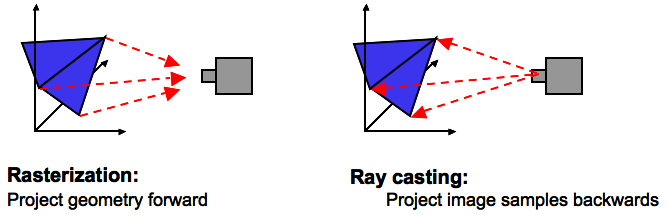
\includegraphics[scale=0.5]{raster}
	\end{center}
	
	\subsection{Problemi}
		Eliminato il calcolo delle intersezioni raggio-oggetto. Ma ho
		molti altri problemi:
		\begin{itemize}
			\item \textbf{Superfici nascoste}: nel ray casting il problema di stabilire quali parti
			della scena sono visibili e quali nascoste viene implicitamente
			risolto: è la prima intersezione lungo il raggio che conta. Nella
			rasterizzazione, quando proietto i poligoni, devo stabilire quali sono
			visibili (e dunque da disegnare) e quali no.
			\item \textbf{Clipping}: nel ray casting gli oggetti al di fuori del volume di vista
			vengono implicitamente scartati. Nella rasterizzazione devo stabilire
			esplicitamente quali poligoni entrano nel volume di vista e quali no.
			Quelli a cavallo vanno tagliati.
			\item \textbf{Scan-conversion}: la proiezione dei poligoni sul piano immagine non
			tiene conto della natura discreta dell’immagine stessa. Alla fine devo
			disegnare un poligono su una matrice di pixel, decidendo dunque
			quali pixel vi appartengono e quali no.
			\item \textbf{Shading interpolativo}: Nel ray casting il colore di ogni pixel deriva
			dall’applicazione del modello di illuminazione al corrispondente
			punto della scena. Nel nuovo paradigma gli unici punti collegati
			esplicitamente a punti della scena sono i vertici dei poligoni. Per
			questi ultimi si può assegnare un colore, e per quelli interni bisogna
			interpolare (abbiamo visto come...).
			\item \textbf{Effetti globali di illuminazione}: Nel ray casting era facile ottenere le
			ombre tracciando gli shadow rays. Più in generale, con il ray-tracing
			si possono ottenere effetti di illuminazione globale che invece nella
			rasterizzazione richiedono trucchi più o meno elaborati (oppure se
			ne fa a meno).
		\end{itemize}
		La soluzione di questi problemi è implementata nella \textbf{pipeline} in modo efficiente e la rasterizzazione risulta più veloce del ray casting.
		
		\bigskip
		
		\begin{center}
			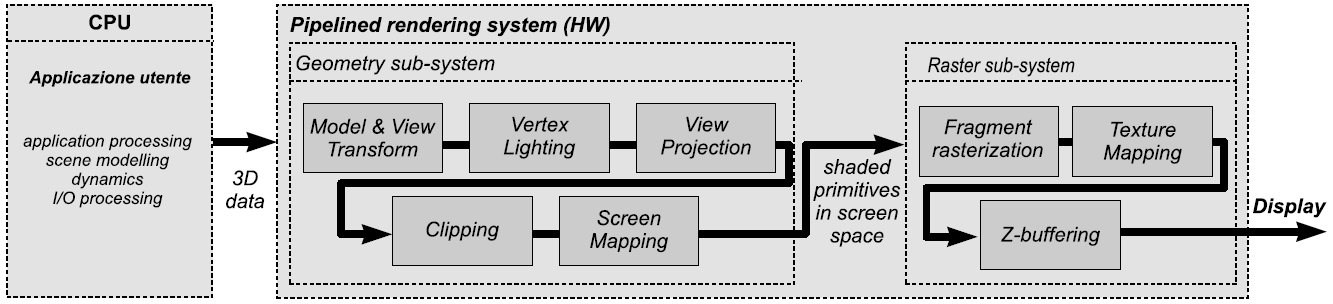
\includegraphics[scale=0.3]{pipeline}
		\end{center}
		
		Avevamo già visto questo schema. Si parte da una lista di primitive (triangoli)
		Si operano una serie di processi a catena (pipeline), parte in CPU, parte in GPU. La pipeline è divisa in due parti: la prima geometrica, la seconda “raster” che lavora sui pixel dell'immagine (la vera rasterizzazione).
		
		\bigskip
				
		In OpenGL possiamo considerare la pipeline grafica come una macchina a stati ove si definiscono delle primitive e delle operazioni che le modificano.\\
		Il programma definisce queste e le passa alla pipeline che dà in ouput le immagini
		Primitive di due tipi: \textbf{geometriche} e \textbf{raster}. Vediamo ora quali sono le operazioni base per realizzare la visualizzazione di una scena triangolata.
	
	
	\subsection{Pipeline geometrica}
		Devo 
		\begin{enumerate}
			\item mettere assieme gli oggetti della scena
			\item rappresentare gli oggetti nel sistema di riferimento della telecamera virtuale. \item Proiettarli. 
			\item Posso applicare le varie trasformazioni geometriche.
		\end{enumerate}
		
		\begin{center}
			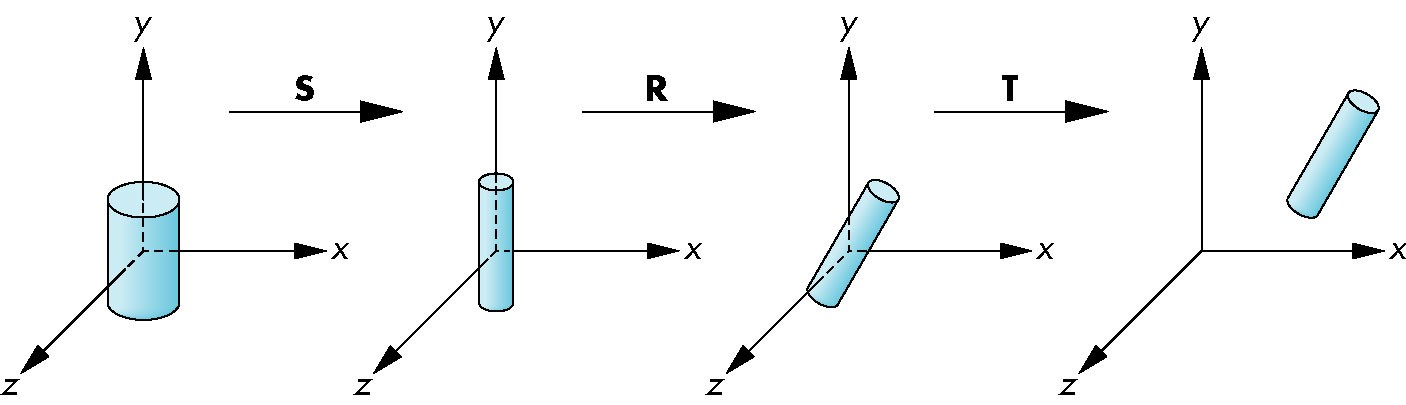
\includegraphics[scale=0.3]{pipelineg}
		\end{center}

		Quindi metto tutti gli oggetti con trasformazioni “di modellazione” (traslazioni, rotazioni, scalature) in un riferimento “coordinate mondo”. Poi devo \textbf{proiettare} sul piano immagine. Avviene quindi una \textbf{proiezione prospettica o affine}.
		
		\begin{center}
			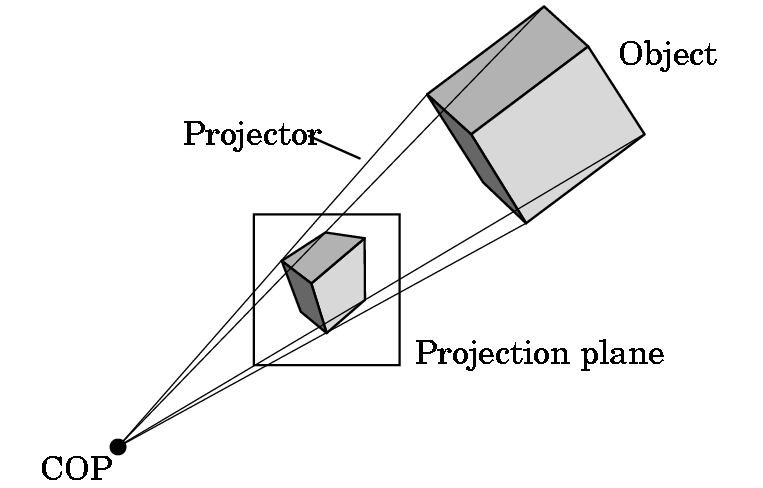
\includegraphics[scale=0.2]{pipelineg1}
			\hspace{1cm}
			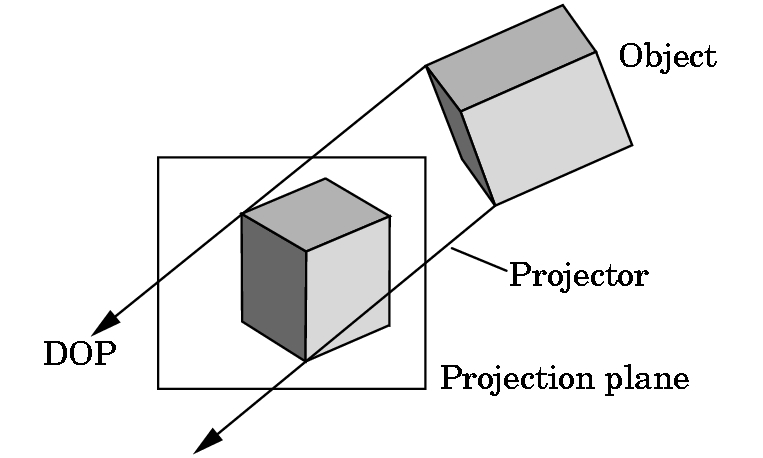
\includegraphics[scale=0.2]{pipelineg2}
		\end{center}
	
	\subsection{Trasformazione di vista}
		Supponiamo di usare la proiezione prospettica. Devo passare in coordinate solidali con la camera (view space, come in figura) e definire cosa “vedo” dato che lavorando in object order devo buttare via il resto (clipping)
		
		\begin{multicols}{2}
			\textbf{Convenzioni:}\\
			Il piano immagine è davanti alla telecamera a distanza $ 1 $ ($ d $ era solo un fattore di scala globale).\\
			L’angolo di vista (solido) si assegna mediante l’angolo di vista (verticale) $ \theta $ ed il fattore di aspetto $ a = w/h $ della finestra di vista.
			
			\columnbreak
			
			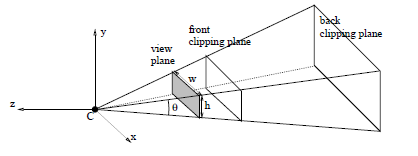
\includegraphics[scale=0.5]{pipelineg3}
			
		\end{multicols}
	
		\noindent
		\textbf{Volume di vista}\\
		La piramide di vista, in principio semi-infinita, viene limitata da due piani paralleli al piano di vista: il piano di taglio anteriore (front clippig plane) e quello posteriore (back clipping plane). Il solido risultante è un frustum, e prende il nome specifico di frustum di vista (view frustum), o volume di vista (view volume). Il frustum di vista è la regione di spazio nel mondo che può apparire sulla finestra di vista.
		
		\begin{center}
			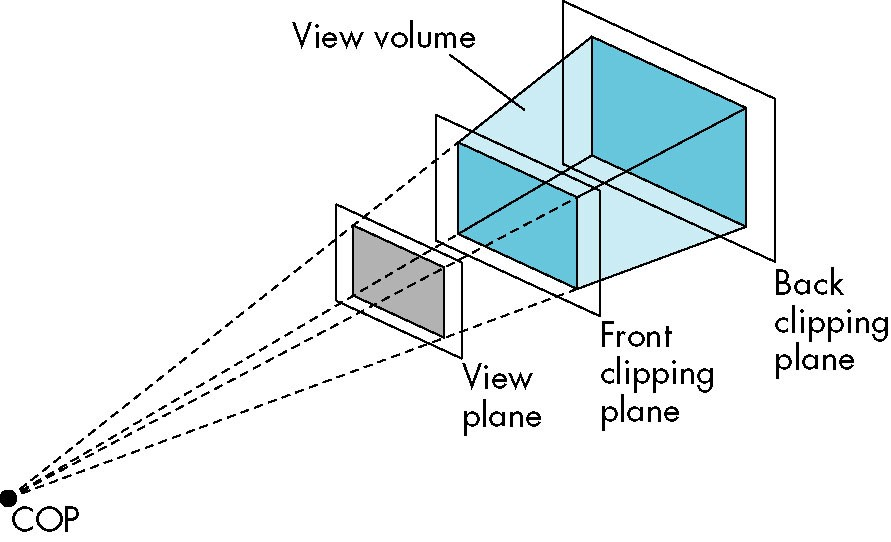
\includegraphics[scale=0.15]{pipelineg4}
		\end{center}
		Gli oggetti che cadono dentro il volume di vista vengono disegnati. Per proiettarli con $ M $ o ($ M_{\perp} $ ) le coordinate devono essere trasformate nello spazio vista, con una trasformazione rigida, detta trasformazione di vista. Si noti che abbiamo messo il piano vista davanti al centro di proiezione, ma l’asse $ Z $ punta “indietro”, quindi la matrice di proiezione rimane la stessa vista prima (con $ d = 1 $):
		\[
			M =
			\begin{pmatrix}
				1 & 0 & 0 & 0 \\
				0 & 1 & 0 & 0 \\
				0 & 0 & -\dfrac{1}{d} & 0
			\end{pmatrix}
		\]
	
	
	\subsection{Trasformazione prospettica}
		\begin{multicols}{2}
			La proiezione prospettica $ M $ potrebbe essere applicata ai punti $ P $ (vertici dei triangoli) espressi nello spazio vista ottenendo le coordinate sul piano immagine.
			Invece si fa una cosa più contorta: si applica la “trasformazione prospettica”, che mappa il frustum in un parallelepipedo retto (volume di vista canonico), poi mappato sul piano immagine con una proiezione ortografica. \\
			Motivo: semplificare le operazioni di clipping (buttar via ciò che sta fuori).
			
			\columnbreak
			
			\begin{center}
				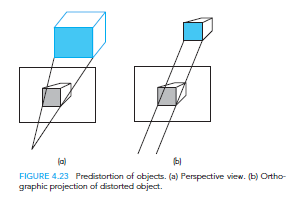
\includegraphics[scale=0.6]{pipelineg5}
			\end{center}
			
		\end{multicols}
	
		Consideriamo la matrice $ 4 \times 4 N $, non singolare (simile alla $ M $) (che prende il nome di matrice di trasformazione o di normalizzazione prospettica).
		\[
			N =
			\begin{pmatrix}
				1 & 0 & 0 & 0 \\
				0 & 1 & 0 & 0 \\
				0 & 0 & \alpha & \beta \\
				0 & 0 & -1 & 0	
			\end{pmatrix}
		\]
		Applicando $ N $ a $ P $ si ottiene la 4-pla $ (x, y, \alpha z + \beta,-z) $ che, dopo la divisione prospettica diventa $ (-x/z,-y/z, -\alpha-\beta/z) $. Le prime due componenti sono identiche alla proiezione standard, ma la terza componente (pseudo-profondità) è diversa: 
		$ z_s = \alpha z +\beta, -z $. per valori di $ \alpha, \beta $ fissati è una funzione monotona di $ z $. La relazione tra $ z $ e $ z_s $ è non lineare, ma l’ordinamento sulla
		profondità è conservato.
	
		\noindent
		\textbf{Volume di vista canonico}\\
		La trasformazione (normalizzazione) prospettica N mappa punti 3D in punti 3D, e scegliendo opportunamente $ \alpha, \beta $ possiamo fare in modo che mappi il frustum di vista in un parallelepipedo con coordinate arbitrarie. Gli oggetti vengono distorti di conseguenza.\\
		Proiettando questo parallelepipedo ortogonalmente (eliminando la terza coordinata, cioè 
		$ z_s $ ) si ottiene la proiezione prospettica desiderata. In OpenGL il volume di vista canonico è un cubo:	$\quad -1\leq x\leq 1 \quad -1\leq y\leq 1  \quad -1\leq z\leq 1 $.
		
		Nel volume di vista canonico il back clipping plane ha equazione $ z_s = 1 $, ed il front clipping plane $ z_s = -1 $. Nel sistema di riferimento camera il front clipping plane di
		trova a distanza $ n $ dall’origine ed il back clipping plane a distanza $ f $.\\
		Vogliamo dunque scegliere $ \alpha, \beta $ in modo che l’intervallo di profondità $ z [-n,-f] $ venga mappato in $ z_s [-1, 1] $ (notare l’inversione di $ z $).
		Si ottiene:
		\[
			\alpha = \dfrac{f + n}{n - f} \quad \beta = -\dfrac{2fn}{n - f}
		\]
	
		Se l’angolo di vista $ \theta = 90 $ ed il fattore d’aspetto $ a = 1 $, allora la matrice $ N $ con $ \alpha , \beta $ calcolati come sopra trasforma il frustum nel volume di vista canonico.
		Nel caso generale, bisogna considerare $ \theta $ e $ a $, moltiplicando $ N $ per la seguente matrice di scalatura, dove $ \gamma = 1/\tan(\theta/2) $ che ha l’effetto di trasformare la piramide generica in piramide retta a base quadrata. Attenzione: questa matrice agisce anche sulle coordinate $ x $ ed $ y $. La matrice $  $ viene chiamata anche (in terminologia OpenGL)
		matrice di proiezione (projection matrix) anche se, a rigore, non effettua una proiezione dello spazio 3D, ma una sua trasformazione.
	
		\textbf{Caso ortogonale}\\
		Se invece si vuole effettuare una proiezione ortogonale (ortografica), basta sostituire la trasformazione prospettica con una trasformazione (affine) che mappa il volume di vista
		(un parallelepipedo in questo caso) nel volume di vista canonico. Nel caso della proiezione ortografica, il volume di vista è già un parallelepipedo, e basta trasformarlo in quello canonico con una opportuna matrice di scalatura.
	
	
	\subsection{Trasformazione viewport}
		\textbf{Viewport}: porzione del display all’interno della quale viene visualizzato il risultato del rendering. La trasformazione viewport si applica dopo la proiezione
		ortografica e dipende dalle caratteristiche fisiche del display. Ai punti proiettati dal volume di vista canonico viene applicata una matrice di trasformazione affine che: 
		\begin{itemize}
			\item ripristina il fattore di aspetto corretto per l’immagine (distorto dalla trasformazione prospettica)
			\item scala e trasla l’immagine.
		\end{itemize}
	
		Quindi la pipeline geometrica coinvolge diversi sistemi di riferimento e trasformazioni tra di essi. In ciascuno di essi avvengono delle operazioni, da parte del codice o della pipeline hardware.
		
		\begin{center}
			\includegraphics[scale=0.5]{pipelineg6}
		\end{center}
		
		Nomi
		I nomi possono variare, ma il senso è quello
	
	
		\textbf{Operazioni}
		\begin{itemize}
			\item \textbf{Clipping}: devo eliminare le parti fuori dal frustum e tagliare i
			poligoni a metà: ricavo lista di poligoni ridotta
			\item \textbf{Illumination}: calcolo il colore con l'equazione semplificata del
			rendering sul vertice (alternativa: farlo dopo)
			\item \textbf{Scan conversion}: trovo i pixel sovrapposti alla proiezione del
			triangolo: genero i frammenti (pixel)
			\item \textbf{Illumination/shading}: calcolo il colore del frammento
			\begin{itemize}
				\item Interpolando i colori dei vertici
				\item Oppure calcolando a questo punto l'illuminazione
			\end{itemize}
			Rimuovo superfici nascoste (Back-face culling).\\
			Mappatura texture, effetti di miscelazione di immagini diverse,
			ecc.
		\end{itemize}

	\subsection{Clipping}
		L’operazione di clipping consiste nell’individuare (e rimuovere) le primitive grafiche (o parti di esse) esterne ad una finestra rettangolare o esaedrale oppure, più in generale,
		esterne ad un poligono o poliedro convesso. In computer graphics si è interessati al clipping rispetto a rettangoli o esaedriClipping (generalità). Non interessa tutto ciò che non è nel view frustumClipping di un punto.\\ 
		\textbf{Clipping di un punto}: un punto è all’interno del rettangolo di .clipping se e solo se sono soddisfatte le 4 disuguaglianze:
		$ x_{min} \leq x \leq x_{max} ,\quad y_{min} \leq y \leq y_{max} $
		
		\begin{tikzpicture}[scale=0.4]
			\draw (2,3) rectangle (6,0); 
			\draw[densely dashed] (0,3) node[left] {$ y = y_{max} $} -- (8,3);
			\draw[densely dashed] (0,0) node[left] {$ y = y_{min} $} -- (8,0);
			\draw[densely dashed] (2,-2)node[below] {$ x = x_{min} $}  -- (2,5);
			\draw[densely dashed] (6,-2)node[below] {$ x = x_{max} $}  -- (6,5);
			\fill (5,2) circle (5pt) coordinate[label=below right:$ P $];
		\end{tikzpicture}

	\noindent
		\textbf{Clipping di un segmento}: necessario analizzare le posizioni dei
		suoi punti estremi.
		\begin{itemize}
			\item Se gli estremi sono entrambi interni al rettangolo di clipping, il
			segmento è interno;
			\item Se un estremo è interno e l’altro esterno, allora il segmento
			interseca il rettangolo di clipping ed è necessario determinare
			l’intersezione;
			\item Se entrambi gli estremi sono esterni al rettangolo, il segmento può
			intersecare o meno il rettangolo di clipping e si rende necessaria
			una analisi più accurata per individuare le eventuali parti interne
			del segmento.
		\end{itemize}
		
		\subsubsection{Algoritmi}
		\textbf{Diretto}: calcolo le intersezioni retta/rettangolo di clipping:
		inefficiente.\\
		\textbf{Cohen-Sutherland}: codifica binaria regioni, in base ai codici
		degli estremi (and logico) capisco le intersezioni.
		
		\begin{tikzpicture}[scale=0.4]
			\draw (2,3) rectangle (6,0); 
			\draw[densely dashed] (0,3) node[left] {$ y = y_{max} $} -- (8,3);
			\draw[densely dashed] (0,0) node[left] {$ y = y_{min} $} -- (8,0);
			\draw[densely dashed] (2,-2)node[below] {$ x = x_{min} $}  -- (2,5);
			\draw[densely dashed] (6,-2)node[below] {$ x = x_{max} $}  -- (6,5);
			\node at (1,4) {1001}; \node at (4,4) {1000}; \node at (7,4) {1010}; 
			\node at (1,1.5) {0001}; \node at (4,1.5) {0000}; \node at (7,1.5) {0010}; 
			\node at (1,-1) {0101}; \node at (4,-1) {0100}; \node at (7,-1) {0110}; 
		\end{tikzpicture}
		
	\textbf{Segmenti: Liang-Barsky}: Un po' più efficiente. 
	\begin{itemize}
		\item Si scrive il segmento in forma parametrica ($ t $ in $ [0 1] $)
		\[
			P_0 +(P_1 - P_0)t= P_0 +t\vec{v}
		\]  
		\item Si trovano le intersezioni con le rette/piani di clipping. 
		\item Si calcolano i valori di t di entrata e uscita dalla regione interna. 
		\item Si trova il segmento dopo clipping prendendo il massimo t dei punti di entrata se >0 e il minimo in uscita (se <1). 
		\item Direttamente applicabile anche in 3D.
	\end{itemize}
	
	\begin{multicols}{2}
		\noindent
		\textbf{Clipping di un poligono}: \\
		è un’operazione più complessa rispetto al clipping di un
	segmento per diversi aspetti: 
	\begin{itemize}
		\item Dal semplice poligono convesso (A);
		\item Al poligono concavo che origina più componenti connesse (B);
		\item In ogni caso il risultato consta di uno o più poligoni e non solo segmenti sconnessi (C).
	\end{itemize}
	
	\columnbreak
	
	\begin{tikzpicture}[>=latex, scale=0.55]
		\draw[fill=Green!50!] (0,4) -- (1,6) -- (3,4) -- cycle;
		\draw[fill=Green!50!] (6,4) -- (8,4) -- (7,5) -- (6,5) -- cycle;
		\draw[fill=Green!50!] (0,2) -- (2.5,2) -- (2.5,0.5) -- (0.5,1.5) -- (0.5,0) -- 
			(2,0) -- (2,-2) -- (0,-2) -- cycle;
		\draw[fill=Green!50!] (6.5,1) -- (7.5,0.5) -- (7.5,1) -- cycle;
		\draw[fill=Green!50!] (6,0) rectangle (7,-1);
		\draw[fill=Green!50!] (1,-3) -- (2,-3) -- (3,-4) -- (1,-4) -- cycle;
		\draw (7,-3) -- (8,-4) -- (6,-4) ;
		
		\draw[thick] (1,5) rectangle (4,3); \draw[thick] (6,5) rectangle (9,3);
		\draw[thick] (1,1) rectangle (4,-1); \draw[thick] (6,1) rectangle (9,-1);
		\draw[dashed] (1,-3) rectangle (4,-5); \draw[dashed] (6,-3) rectangle (9,-5);
		
		\draw[->] (4.5,4) -- (5.5,4); \draw[->] (4.5,0) -- (5.5,0);
		
		\node[below] at (5,3) {A}; \node[below] at (5,-1) {B}; \node[below] at (5,-5) {C};
	\end{tikzpicture}
	\end{multicols}
	
	\noindent
	L’approccio \textbf{diretto} consiste nel confrontare ogni lato del poligono con le 4 rette che delimitano il rettangolo di clipping; Questo approccio implica l’esecuzione di operazioni costose (la determinazione di intersezioni) e spesso inutili. 
	
	\noindent
	\textbf{Clipping di un poligono (Sutherland-Hodgman)}:\\
	Approccio divide et impera; Il problema è ricondotto al clipping di un poligono generico rispetto ad una retta; La procedura è applicata sequenzialmente alle 4 rette che definiscono il Poligono originale rettangolo di clipping.
	
	\noindent
	\textbf{Clipping con bounding box}
	Altro approccio: calcolo la bounding box della primitiva
	Considero intersezione tra bounding box e regione di vista
	Solo se le regioni si intersecano faccio clipping
	(sull'intersezione).
	
	\subsection{Rimozione superfici nascoste (HSR)}
	Gli oggetti della scena sono generalmente opachi;\\
	Gli oggetti più vicini all’osservatore possono nascondere (occludere) la vista (totale o parziale) di oggetti più lontani; Il problema della rimozione delle superfici nascoste (\textbf{HSR, Hidden surface removal}) consiste nel determinare le parti della
	scena non visibili dall’osservatore;\\
	La rimozione delle superfici nascoste non è solo dipendente dalla disposizione degli oggetti nella scena ma anche dalla relazione esistente tra oggetti e posizione dell’osservatore.\\
	Quindi in una applicazione interattiva se sposto il punto di vista cambia la visibilità degli oggetti.
	
	\bigskip
	
	Stiamo analizzando la parte “geometrica” della pipeline grafica. La rimozione però non è necessariamente fatta qui:
	\begin{itemize}
		\item Algoritmi che operano in object-space determinano, per ogni primitiva geometrica della scena, le parti della primitiva che non risultano oscurate da altre primitive nella scena. Gli algoritmi operano nello spazio di definizione delle primitive;
		
		[Applicazione o Geometry subsystem]
		
		\item Algoritmi che operano in image-space determinano, per ogni punto “significativo” del piano di proiezione (ogni pixel del piano del piano immagine), la primitiva geometrica visibile “attraverso” quel punto. Gli algoritmi operano nello spazio immagine della scena proiettata.
		
		[Raster subsystem]
	\end{itemize}
	
	
	\textit{Conviene operare in object space?}\\
	Nell’ipotesi di una scena 3D composta da k primitive geometriche planari ed opache, si può derivare un generico algoritmo di tipo object-space analizzando gli oggetti a coppie;
	Fissato un punto di vista, le relazioni spaziali di due primitive geometriche A e B possono essere:
	\begin{itemize}
		\item $ A [B] $ oscura $ B [A] $; solo $ A [B] $ è visualizzata;
		\item $ A $ e $ B $ sono completamente visibili; entrambe le primitive sono
		visualizzate;
		\item $ A [B] $ occlude parzialmente $ B [A] $
	\end{itemize}
	è necessario individuare le parti visibili di $ B [A] $.
%	HSR: Object-space
%	A oscura B: tutti i punti di A
%	sono più vicini
%	all’osservatore di tutti i
%	punti di B e la proiezione di
%	B sul piano di vista ricade
%	all’interno della proiezione di
%	A. Visualizza A;
%	B oscura A: tutti i punti di B
%	sono più vicini
%	all’osservatore di tutti i
%	punti di A e la proiezione di
%	A sul piano di vista ricade
%	all’interno della proiezione di
%	B. Visualizza B.
%	A
%	BHSR: Object-space
%	A e B non si occludono: le
%	due proiezioni di A e B sul
%	piano di vista sono disgiunte;
%	Visualizza A e B.
%	A
%	BHSR: Object-space
%	A e B si oscurano
%	parzialmente:
%	l’intersezione tra le due
%	proiezioni di A e B sul piano
%	di vista è non nulla e diversa
%	sia dalla proiezione di A che
%	da quella di B.
%	Individua le parti visibili di
%	ciascuna primitiva.
%	A
%	B
%	A
%	BHSR: Object-space
%	Un possibile algoritmo risolutivo:
%	Proiettare le k primitive geometriche;
%	Al generico passo analizzare la i-esima primitiva (i=1, ..., k-1) con le
%	rimanenti k   –   i in modo da individuare le parti visibili.
%	La complessità dell’approccio object-space risulta di ordine
%	O(k 2 )
%	L’approccio object-space è consigliabile solo quando le
%	primitive nella scena sono relativamente poche.
%	Si può aumentare l'efficienza?Sì ricordiamo le tecniche di suddivisione spaziale
%	Riorganizzare gli oggetti della scena (o le loro proiezioni sul piano
%	immagine) in gruppi coerenti dal punto di vista spaziale;
%	Si effettua di solito mediante griglie 2D o 3D che servono a limitare i
%	confronti in profondità tra le primitive della scena.
%	Ma per oggetti con molti triangoli resterebbe
%	Quindi normalmente l'operazione viene fatta a livello in image
%	space, cioé nella parte di pipeline che vedremo nella prossima
%	lezione, cioè a livello dei pixelHSR: Image-space
%	E' quello che normalmente si
%	fa nella pipeline grafica
%	In pratica si tratta di
%	ordinare per profondità le
%	proiezioni delle primitive su
%	ciascun pixel dell'immagine
%	finale e tenere solo la
%	proiezione che avviene da
%	più vicino
%	La rimozione delle superfici
%	occluse è sempre un
%	ordinamento per distanza
%	lungo il proiettoreHSR: Image-space
%	L’operazione fondamentale dell’approccio image-space è il
%	calcolo delle intersezioni tra semirette e piani di
%	appartenenza delle primitive (per ogni semiretta al più k
%	intersezioni);
%	Anche se per un display n x m, questa operazione deve essere
%	eseguita n x m x k volte, la complessità risulta comunque di
%	ordine O(k)
%	Sia nell’approccio object-space che in quello image-space la
%	rimozione delle superfici nascoste è riconducibile ad un
%	problema di ordinamento (in profondità).Con e senza rimozione superfici
%	nascosteBack-face culling
%	Alcune facce invisibili sono più facilmente rimosse
%	Back-face culling (Eliminazione delle facce posteriori)
%	Se gli oggetti della scena sono rappresentati da poliedri solidi
%	chiusi (cioè le facce poligonali dei poliedri delimitano
%	completamente i volumi dei solidi);
%	Se ogni faccia poligonale è stata modellata in modo tale che la
%	normale ad essa sia diretta verso l’esterno del poliedro di
%	appartenenza;
%	Se nessuna parte del poliedro viene tagliata dal front clipping
%	plane ...Back-face culling
%	Nelle ipotesi precedenti...
%	Le facce la cui normale
%	forma angoli superiori a
%	±90° con la direzione di
%	vista possono essere visibili;
%	Le facce la cui normale
%	forma angoli inferiori a ±90°
%	con la direzione di vista
%	certamente non sono
%	visibili ;Back-face culling
%	Per ridurre il carico di lavoro richiesto per la rimozione delle
%	superfici nascoste può essere quindi opportuno eliminare
%	inizialmente tutti le primitive geometriche la cui normale è
%	orientata verso il semispazio opposto all’osservatore, non
%	visibile all’osservatore;
%	Indicato con  l’angolo tra la normale e l’osservatore, la
%	primitiva in esame deve essere rimossa se -90°    90°,
%	cioè se cos   0.
%	Invece di calcolare la quantità
%	cos  possiamo valutare il
%	prodotto scalare n·v  0Back-face culling
%	Se l’operazione è eseguita in coordinate normalizzate di vista
%	(dopo aver eseguito la proiezione) la determinazione delle
%	facce back-facing si riduce ad un controllo del segno della
%	coordinata z delle normali: ad un segno positivo
%	corrispondono facce front-facing, ad un segno negativo facce
%	back-facing;
%	Questo procedimento (detto back-face culling) consente, in
%	media, di dimezzare il tempo necessario per il rendering di
%	oggetti solidi dato che, sempre in media, circa metà delle
%	facce di un poliedro sono back-facing e quindi la loro
%	visualizzazione sarebbe comunque inutile.Riepilogo
%	Spazio Oggetto (object space): dove ciascun singolo oggetto viene
%	·
%	·
%	·
%	·
%	definito. Detto anche local space o modeling space
%	Spazio Mondo (world space): dove si costruisce. Si passa dallo spazio
%	oggetto allo spazio mondo mediante la trasformazione di modellazione.
%	Si chiama anche application space.
%	Spazio Vista (view space): centrato sulla telecamera virtuale, che
%	definisce, assieme alla finestra di vista ed ai piani di taglio, il frustum di
%	vista. Detto anche camera space o eye space
%	Spazio schermo 3-D (3D-screen space): volume di vista canonico, che si
%	ottiene trasformando il frustum di vista in un parallelepipedo. Molte
%	operazioni del processo di rendering avvengono qui. Detto anche 3D
%	normalized device coordinate system (NDC) o normalized projection
%	coordinate system.
%	Spazio Immagine (image space): sistema di coordinate nel display fisico
%	(pixel). Si ottiene proiettando ortogonalmente il volume di vista
%	canonico ed applicando la trasformazione di viewport. Si chiama anche
%	(physical) device coordinate system, o screen coordinate system.
%	
%	
%	A questo punto
%	Abbiamo mappato i triangoli sul piano immagine nella regione
%	del “sensore” della telecamera virtuale
%	Abbiamo eliminato le parti esterne al volume di vista (e in
%	parte eliminato le parti occluse)
%	Ora dobbiamo sovrapporre i triangoli ai pixel dell'immagine
%	discretizzata e colorare i pixel corrispondenti sulla base di
%	modello di illuminazione e caratteristiche della geometria
%	Questo è compito della seconda parte della pipeline cioè del
%	cosiddettto “raster” subsystem
	
\end{document}	